\chapter{The response framework}\label{chap:8}
A particle with a magnetic moment couples to the charge of a solid and also to its spins and currents, and a fermion that is absorbed leaves a light partner behind; neither the magnetic coupling nor the fermion absorption fits the single product of \cref{eq:1.1-rate}, a halo factor times a coupling $|\tilde V|^2$ times one dynamic structure factor. So far \cref{chap:4} took the electron density of silicon, \cref{chap:5} the nuclei of a harmonic crystal, \cref{chap:6} electrons and lattice together, and \cref{chap:7} the spins of NiO and the paired electrons of aluminum. A new model or a new target should not mean starting again. What do these calculations have in common, and what does each of them leave out?

Every model reduces to a tensor that weights the response matrix of a few target operators, and every target to that one matrix. A new model then needs a new tensor but not a new matrix, and a new target needs a new matrix but not a new tensor. Because the matrix belongs to the target alone, three questions about it can be settled once, for every coupling at the same time: what is exact about the matrix, how the medium screens it, and where a calculation truncates it. We will build this framework (\cref{fig:8-map}) from the separate results of \crefrange{chap:1}{chap:7}, up to the final state that the dark matter leaves in the target. Each truncation on the way leaves in the rate a theory uncertainty of known size and shape.

\begin{figure}[tbp]
  \centering
  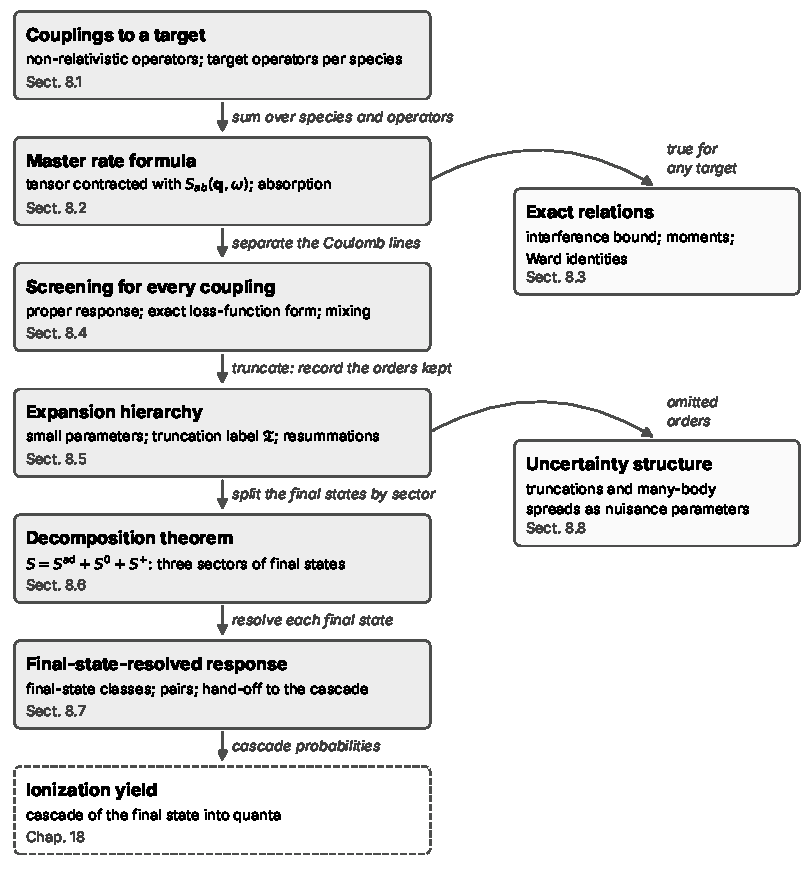
\includegraphics[width=0.85\linewidth]{figures/ch08/map08.pdf}
  \caption{The response framework from couplings to final states. The non-relativistic operators of every model reduce to target operators per species (\cref{sec:8.1}), and the master rate formula contracts a dark-matter tensor with the response matrix $S_{ab}(\vect{q},\omega)$ (\cref{sec:8.2}), which obeys exact relations for any target (\cref{sec:8.3}). Separating the Coulomb lines screens every coupling (\cref{sec:8.4}); the truncation label records the orders a calculation keeps (\cref{sec:8.5}). The decomposition theorem splits the final states into three sectors (\cref{sec:8.6}), and the final-state-resolved response divides each sector by the class of its final state (\cref{sec:8.7}). The omitted orders and many-body spreads of the truncation label become theory uncertainties (\cref{sec:8.8}).}
  \label{fig:8-map}
\end{figure}

\section{Dark-matter couplings to a target}\label{sec:8.1}

A dark photon couples to a solid through its charge alone. In the language of \cref{sec:4.2} it needs one target operator per species, the electron density $n_e(\vect{q})$ and the density $n_\kappa(\vect{q})$ of each kind of nucleus, with potentials of opposite sign. A dark-matter particle with a magnetic dipole moment does more: it feels the spins of the electrons, and, since a charge moving past a magnetic moment feels a force, their velocities as well~\cite[Table~II]{trickle2022effective}. Particle physics offers many such models, and at first sight each would need its own calculation of the target. None does. A slow dark-matter particle sees an electron or a nucleus through three things only: the momentum it hands over, the velocity of the two particles relative to each other, and their spins. As a result every model reduces to the same short list of target operators per species: the density, the spin density, the current, the spin current and a kinetic-energy density. What remains of the model is a tensor on the dark-matter side that weights the response matrix of these operators.

\subsection{The non-relativistic operators}

Take a dark-matter particle of mass $\mchi$ and spin operator $\vect{S}_\chi$ that scatters on a free electron, with spin $\vect{S}_e = \boldsymbol{\sigma}/2$. The dark matter goes from $\vect{p}$ to $\vect{p}' = \vect{p} - \vect{q}$ and the electron from $\vect{k}$ to $\vect{k}' = \vect{k} + \vect{q}$, with $\vect{q}$ the momentum transfer of \cref{sec:1.3}. Momentum conservation leaves three of the four momenta independent, and Galilean invariance, the freedom to add a common velocity to both particles, allows an interaction to depend on them only through $\vect{q}$ and one velocity difference~\cite[Sect.~2.2]{fitzpatrick2013effective}. The difference that is Hermitian, symmetric between the incoming and outgoing particles, is
\begin{equation}
  \vect{v}^\perp = \bar{\vect{v}}_\chi - \frac{\vect{k} + \vect{k}'}{2m_e}, \qquad
  \bar{\vect{v}}_\chi \equiv \frac{\vect{p} + \vect{p}'}{2\mchi} = \vect{v} - \frac{\vect{q}}{2\mchi} ,
  \label{eq:8.1-vperp}
\end{equation}
the mean velocity of the dark matter minus that of the electron, with $\vect{v} = \vect{p}/\mchi$ the incoming velocity. For an electron initially at rest, $\vect{v}^\perp = \vect{v} - \vect{q}/2\mu_{\chi e}$, and energy conservation in the form $\vect{q}\cdot\vect{v} = q^2/2\mu_{\chi e}$ (\cref{sec:1.3}) makes $\vect{q}\cdot\vect{v}^\perp = 0$. This transversality is the origin of the name~\cite[Eq.~(14)]{fitzpatrick2013effective}, and \cref{app:D.24} shows that it holds for any free target. The momentum enters as $\ii\vect{q}$. Hermitian conjugation exchanges the incoming and outgoing particles, which reverses $\vect{q}$ and leaves $\vect{v}^\perp$ unchanged, so that $\ii\vect{q}$, $\vect{v}^\perp$ and the spins are all Hermitian.

An interaction is then a scalar built from $\ii\vect{q}$, $\vect{v}^\perp$, $\vect{S}_\chi$ and $\vect{S}_e$. Powers of $q^2$ can be absorbed into a momentum-dependent coefficient, as the mediator propagator of \cref{eq:1.4-Vq} already is, and products of more than one spin of the same particle reduce to at most one by the algebra of the Pauli matrices~\cite[Sect.~2.2]{fitzpatrick2013effective}. What remains is a finite list of operators, which Fitzpatrick and collaborators wrote down and Anand, Fitzpatrick and Haxton completed~\cites[Eqs.~(19)--(24) and (45)]{fitzpatrick2013effective}[Eqs.~(12) and (13)]{anand2014model}. They are listed in \cref{tab:8-operators}, which writes $\vect{q}/m_e$ in place of $\vect{q}$, so that each operator is dimensionless. The list is complete for dark matter of spin $\frac12$, whose spin products the Pauli algebra reduces. For spin 1 a product of two dark-matter spins leaves a symmetric tensor built from the polarization vectors, and two more operators appear, $\vect{q}$ contracted through that tensor with $\vect{v}^\perp$ or with $\vect{S}_e$~\cite[Eq.~(18)]{dent2015general}; for spin 0 only the operators free of $\vect{S}_\chi$ remain. The target side does not change: the new operators are linear in the electron's velocity or spin and reduce to the same rows. The potential between the dark matter and the electron is a sum
\begin{equation}
  \tilde V(\vect{q}) = \sum_i c_i^{(e)}(q)\,\mathcal{O}_i^{(e)} ,
  \label{eq:8.1-eft}
\end{equation}
an operator in the spin spaces of both particles, whose matrix element between plane waves is the transition amplitude in the first Born approximation (\cref{sec:2.2}). The coefficients $c_i^{(e)}(q)$ carry the dimension $\mathrm{eV}^{-2}$ of $\tilde V$ and the momentum dependence of the mediator. For the Yukawa potential of \cref{sec:1.4}, $c_1^{(e)}(q) = \tilde V(q) = y_\chi y_e/(q^2 + m_V^2)$, and every other coefficient vanishes. Papers that normalize their states relativistically quote $4\mchi m_e\,c_i^{(e)}$ instead, the factor of \cref{eq:A.9-M}. Refs.~\cite{fitzpatrick2013effective,anand2014model} define $\vect{q}$ as the momentum the dark matter gains, the opposite of the $\vect{q}$ of this book, so a coefficient quoted there changes sign for the operators odd in $\vect{q}$, $i = 3, 5, 9, 10, 11, 13, 14$; $\vect{v}^\perp$ is the same in both conventions.

Which operators a model produces follows from the non-relativistic limit of its couplings. The limits of the four Dirac bilinears are derived in \cref{app:C.15} and, between plane waves, in \cref{app:D.24}. The scalar $\bar\psi\psi$ and the time component of the vector $\bar\psi\gamma^\mu\psi$ both reduce to the density, $1$. The spatial vector reduces to the velocity plus a spin term, $(\vect{k} + \vect{k}')/2m_e - \ii\vect{q}\times\vect{S}_e/m_e$, the spatial axial vector $\bar\psi\gamma^\mu\gamma^5\psi$ to twice the spin, $2\vect{S}_e$, and the pseudoscalar $\bar\psi\ii\gamma^5\psi$ to $-\ii\vect{q}\cdot\vect{S}_e/m_e$. Multiplying a dark-matter bilinear by an electron bilinear and by the mediator propagator gives the coefficients. A vector mediator coupled to both vector currents leads to $\mathcal{O}_1$, and an axial-vector mediator coupled to both axial currents to $\mathcal{O}_4$, the standard spin-independent and spin-dependent interactions. A scalar mediator with a pseudoscalar coupling to the electron produces $\mathcal{O}_{10}$, and with pseudoscalar couplings on both sides $\mathcal{O}_6$. Dark matter with an electric dipole moment that couples through a photon-like mediator produces $\mathcal{O}_{11}$; a magnetic dipole moment, $\mathcal{O}_1$, $\mathcal{O}_4$, $\mathcal{O}_5$ and $\mathcal{O}_6$; and an anapole moment, $\mathcal{O}_8$ and $\mathcal{O}_9$~\cite[Table~II]{trickle2022effective}. The dipole and anapole couplings bring extra powers of $q$, in the operator or in the coefficient, and those coupled through a light mediator are strongly weighted toward small $q$. Operator $\mathcal{O}_2 = (\vect{v}^\perp)^2$ arises in none of these models at leading order~\cite[Sect.~2.1]{anand2014model}. It appears as a correction, of relative size $v^2$, to $\mathcal{O}_1$, and many lists omit it~\cite[Table~I]{catena2021crystal}; we keep it, because its reduction needs a row that the scalar absorption of \cref{sec:8.1-absorption} needs anyway.

\subsection{Target operators per species}

Inside a crystal the electron that the dark matter strikes is one of $10^{23}$, bound by the nuclei and by the other electrons, and its bare momentum $\vect{k}$ is not conserved; only its crystal momentum is (\cref{chap:3}). What survives is the structure of \cref{eq:8.1-eft}. Each operator acts on the target particle through three ingredients, the phase $\ee^{\ii\vect{q}\cdot\vect{r}}$ that adds the momentum $\vect{q}$, the velocity $(\vect{k} + \vect{k}')/2m_e$ inside $\vect{v}^\perp$, and the spin $\vect{S}_e$, and each has a one-body operator whose matrix elements between plane waves reproduce it. The phase is $\ee^{\ii\vect{q}\cdot\vect{r}}$ itself. The velocity is the symmetrized product $\tfrac12\{\vect{p}/m_e, \ee^{\ii\vect{q}\cdot\vect{r}}\}$, whose element from $\vect{k}$ to $\vect{k}'$ is $(\vect{k} + \vect{k}')/2m_e$, since $\vect{p}$ acting to the left gives $\vect{k}'$ and to the right gives $\vect{k}$. The square of the velocity is the doubly symmetrized $\{\vect{p}, \{\vect{p}, \ee^{\ii\vect{q}\cdot\vect{r}}\}\}/4m_e^2$. Summing over the particles, as in \cref{eq:2.3-onebody}, leads to five operators. Let $s$ be a species, either the electrons ($s = e$) or the nuclei of species $\kappa$ ($s = \kappa$), with mass $m_s$. Its particles $j$ have positions $\vect{r}_j$, momenta $\vect{p}_j$ and spins $\vect{S}_j$, and
\begin{keyresult}[Target operators per species]
\begin{equation}
  \begin{gathered}
  \begin{aligned}
  n_s(\vect{q}) &= \sum_{j\in s}\ee^{\ii\vect{q}\cdot\vect{r}_j}, &
  \vect{s}_s(\vect{q}) &= \sum_{j\in s}\ee^{\ii\vect{q}\cdot\vect{r}_j}\,\vect{S}_j, \\
  \vect{j}_s(\vect{q}) &= \sum_{j\in s}\frac12\Bigl\{\frac{\vect{p}_j}{m_s},\,\ee^{\ii\vect{q}\cdot\vect{r}_j}\Bigr\}, &
  \mathcal{J}^{\alpha\beta}_s(\vect{q}) &= \sum_{j\in s}\frac12\Bigl\{\frac{p^\alpha_j}{m_s},\,\ee^{\ii\vect{q}\cdot\vect{r}_j}\Bigr\}\,S^\beta_j,
  \end{aligned}\\
  \mathcal{T}_s(\vect{q}) = \sum_{j\in s}\frac{1}{8m_s}\bigl\{\vect{p}_j, \{\vect{p}_j, \ee^{\ii\vect{q}\cdot\vect{r}_j}\}\bigr\}
  = \sum_{j\in s}\frac{\vect{p}_j\cdot\ee^{\ii\vect{q}\cdot\vect{r}_j}\,\vect{p}_j}{2m_s} + \frac{q^2}{8m_s}\,n_s(\vect{q}) .
  \end{gathered}
  \label{eq:8.1-rows}
\end{equation}
These are the density, the spin density, the paramagnetic current, the spin current (velocity index $\alpha$, spin index $\beta$) and the kinetic-energy density. Their matrix elements from a plane wave $\vect{k}$ to $\vect{k} + \vect{q}$ are $1$, $\vect{S}$, $(\vect{k} + \vect{k}')/2m_s$, $(k^\alpha + k'^\alpha)S^\beta/2m_s$ and $(\vect{k} + \vect{k}')^2/8m_s$.
\end{keyresult}
\noindent For the electrons they are old acquaintances. The density $n_e(\vect{q})$ is \cref{eq:2.3-nq}, the spin density $\vect{s}_e(\vect{q})$ is \cref{eq:7.1-se}, and the current $\vect{j}_e(\vect{q})$ is that of the continuity equation \cref{eq:4.3-continuity}. The spin current and the kinetic-energy density are new. At $\vect{q} = 0$ the kinetic-energy density is the kinetic energy $\sum_j p_j^2/2m_s$ of the species, and at finite $\vect{q}$ it is the kinetic energy of the mean of the incoming and outgoing momenta, which is why the term $q^2/8m_s$ appears beside the familiar $\vect{p}\cdot\ee^{\ii\vect{q}\cdot\vect{r}}\vect{p}/2m_s$. For nuclei the spin $\vect{S}_j$ is the nuclear spin, and \cref{sec:8.1-nuclei} turns couplings to nucleons into couplings to these rows.

With the rows in hand the reduction is mechanical. Substitute $\vect{v}^\perp = \bar{\vect{v}}_\chi - (\vect{k} + \vect{k}')/2m_e$ in each operator, expand, and replace every monomial in the electron's velocity and spin by its row: $1 \to n_e$, $\vect{S}_e \to \vect{s}_e$, the velocity $\to \vect{j}_e$, the velocity times the spin $\to \mathcal{J}_e$, and the square of the velocity $\to (2/m_e)\mathcal{T}_e$. The dark-matter velocity $\bar{\vect{v}}_\chi$ and spin $\vect{S}_\chi$ are not target operators; they stay in the coefficients. For instance,
\begin{equation}
  \mathcal{O}_8 = \vect{S}_\chi\cdot\vect{v}^\perp \;\to\; (\vect{S}_\chi\cdot\bar{\vect{v}}_\chi)\,n_e(\vect{q}) - \vect{S}_\chi\cdot\vect{j}_e(\vect{q}) ,
  \qquad
  \mathcal{O}_7 = \vect{S}_e\cdot\vect{v}^\perp \;\to\; \bar{\vect{v}}_\chi\cdot\vect{s}_e(\vect{q}) - \mathcal{J}^{\alpha\alpha}_e(\vect{q}) ,
  \label{eq:8.1-O7O8}
\end{equation}
with a sum over the repeated Cartesian index. \Cref{tab:8-operators} lists all fifteen reductions, and \cref{app:D.24} derives them. Every operator except $\mathcal{O}_2$ is at most linear in the electron's velocity and in its spin, and needs at most the four rows $n_e$, $\vect{s}_e$, $\vect{j}_e$ and $\mathcal{J}_e$~\cite[Table~III]{trickle2022effective}; $\mathcal{O}_2$ adds $\mathcal{T}_e$.

\begin{table}[tbp]
  \caption{Non-relativistic operators of dark-matter scattering and absorption, and the target operators each needs. Upper block: the operators $\mathcal{O}_i$ of Refs.~\cite[Eqs.~(19)--(24) and (45)]{fitzpatrick2013effective} and~\cite[Eqs.~(12) and (13)]{anand2014model}, written for an electron with $\vect{q}$ the momentum the dark matter loses; $\vect{v}^\perp$ is \cref{eq:8.1-vperp}, $\bar{\vect{v}} \equiv \bar{\vect{v}}_\chi = \vect{v} - \vect{q}/2\mchi$, and $m = m_e$. The rows are those of \cref{eq:8.1-rows} for $s = e$, all at the same $\vect{q}$; repeated Cartesian indices are summed, and $\epsilon_{\alpha\beta\gamma}$ is the Levi-Civita symbol. For nucleons, replace $e$ by $N$ and $m_e$ by the nucleon mass; the nuclear rows follow from \cref{eq:8.1-nuclear}. Lower block: absorption of a boson $\phi$ of mass $m_\phi$ at $\vect{q} = \vect{p}_\phi$, and fermionic absorption with an outgoing fermion $\tilde\nu$ (\cref{sec:8.1-absorption}). Last column: what each row excites in an insulator. Through the nuclei the density row also excites phonons, and in an ordered magnet the spin rows excite magnons (\cref{sec:7.1}).}
  \label{tab:8-operators}
  \centering\small
  \renewcommand{\arraystretch}{1.25}
  \begin{tabular}{@{}l>{\raggedright\arraybackslash}p{0.25\linewidth}>{\raggedright\arraybackslash}p{0.39\linewidth}>{\raggedright\arraybackslash}p{0.15\linewidth}@{}}
    \toprule
    & Operator & Target operators & Excites \\
    \midrule
    $\mathcal{O}_1$ & $1$ & $n$ & pairs, plasmons \\
    $\mathcal{O}_2$ & $(\vect{v}^\perp)^2$ & $\bar v^2 n - 2\bar{\vect{v}}\cdot\vect{j} + (2/m)\mathcal{T}$ & pairs \\
    $\mathcal{O}_3$ & $\ii\vect{S}_e\cdot(\vect{q}/m\times\vect{v}^\perp)$ & $(\ii/m)\bigl[(\vect{q}\times\bar{\vect{v}})\cdot\vect{s} - \epsilon_{\alpha\beta\gamma}q^\beta\mathcal{J}^{\gamma\alpha}\bigr]$ & spin flips \\
    $\mathcal{O}_4$ & $\vect{S}_\chi\cdot\vect{S}_e$ & $\vect{S}_\chi\cdot\vect{s}$ & spin flips \\
    $\mathcal{O}_5$ & $\ii\vect{S}_\chi\cdot(\vect{q}/m\times\vect{v}^\perp)$ & $(\ii/m)\,\vect{S}_\chi\cdot\bigl[(\vect{q}\times\bar{\vect{v}})\,n - \vect{q}\times\vect{j}\bigr]$ & pairs \\
    $\mathcal{O}_6$ & $(\vect{S}_\chi\cdot\vect{q}/m)(\vect{S}_e\cdot\vect{q}/m)$ & $(\vect{S}_\chi\cdot\vect{q})(\vect{q}\cdot\vect{s})/m^2$ & spin flips \\
    $\mathcal{O}_7$ & $\vect{S}_e\cdot\vect{v}^\perp$ & $\bar{\vect{v}}\cdot\vect{s} - \mathcal{J}^{\alpha\alpha}$ & spin flips \\
    $\mathcal{O}_8$ & $\vect{S}_\chi\cdot\vect{v}^\perp$ & $(\vect{S}_\chi\cdot\bar{\vect{v}})\,n - \vect{S}_\chi\cdot\vect{j}$ & pairs \\
    $\mathcal{O}_9$ & $\ii\vect{S}_\chi\cdot(\vect{S}_e\times\vect{q}/m)$ & $(\ii/m)\,\vect{S}_\chi\cdot(\vect{s}\times\vect{q})$ & spin flips \\
    $\mathcal{O}_{10}$ & $\ii\vect{S}_e\cdot\vect{q}/m$ & $(\ii/m)\,\vect{q}\cdot\vect{s}$ & spin flips \\
    $\mathcal{O}_{11}$ & $\ii\vect{S}_\chi\cdot\vect{q}/m$ & $(\ii/m)(\vect{S}_\chi\cdot\vect{q})\,n$ & pairs \\
    $\mathcal{O}_{12}$ & $\vect{S}_\chi\cdot(\vect{S}_e\times\vect{v}^\perp)$ & $\vect{S}_\chi\cdot(\vect{s}\times\bar{\vect{v}}) - \epsilon_{\alpha\beta\gamma}S^\alpha_\chi\mathcal{J}^{\gamma\beta}$ & spin flips \\
    $\mathcal{O}_{13}$ & $\ii(\vect{S}_\chi\cdot\vect{v}^\perp)(\vect{S}_e\cdot\vect{q}/m)$ & $(\ii/m)\bigl[(\vect{S}_\chi\cdot\bar{\vect{v}})(\vect{q}\cdot\vect{s}) - S^\alpha_\chi q^\beta\mathcal{J}^{\alpha\beta}\bigr]$ & spin flips \\
    $\mathcal{O}_{14}$ & $\ii(\vect{S}_\chi\cdot\vect{q}/m)(\vect{S}_e\cdot\vect{v}^\perp)$ & $(\ii/m)(\vect{S}_\chi\cdot\vect{q})\bigl(\bar{\vect{v}}\cdot\vect{s} - \mathcal{J}^{\alpha\alpha}\bigr)$ & spin flips \\
    $\mathcal{O}_{15}$ & $-(\vect{S}_\chi\cdot\vect{q}/m)\bigl[(\vect{S}_e\times\vect{v}^\perp)\cdot\vect{q}/m\bigr]$ & $-(\vect{S}_\chi\cdot\vect{q})\bigl[\vect{q}\cdot(\vect{s}\times\bar{\vect{v}}) - \epsilon_{\alpha\beta\gamma}q^\alpha\mathcal{J}^{\gamma\beta}\bigr]/m^2$ & spin flips \\
    \midrule
    Dark photon & $-\zeta e\,A'_\mu J^\mu_{\mathrm{em}}$ & $-\vect{j}_e + \sum_\kappa Z_\kappa\vect{j}_\kappa$ & pairs; polar phonons \\
    ALP & $g_{aee}\,\phi\,\bar\psi\ii\gamma^5\psi$ & $\vect{s}_e$ ($\propto|\vect{p}_\phi|$); $\mathcal{J}^{\alpha\alpha}_e$ ($\propto m_\phi$) & pairs \\
    Scalar & $g_{\phi ee}\,\phi\,\bar\psi\psi$ & $n_e - \mathcal{T}_e/m_e$ & pairs \\
    Fermionic & $\Lambda_F^{-2}(\bar{\tilde\nu}\Gamma\chi)(\bar\psi\Gamma'\psi)$ & $n$, $\vect{j}$, $\vect{s}$, $\mathcal{J}^{\alpha\alpha}$ or $n - \mathcal{T}/m$, by $\Gamma'$ & pairs; nuclear recoils \\
    \bottomrule
  \end{tabular}
\end{table}

In a solid the electron moves too. The velocity-dependent operators split into a piece in which the dark-matter velocity multiplies a velocity-independent row and a piece that needs the target's own velocity. For a free electron at rest the second piece vanishes, but in a solid it does not, and it is often the larger: the valence electrons of silicon, taken as a free gas at their density, move at $v_{\mathrm{F}} = k_{\mathrm{F}}/m_e = 7.0\times10^{-3}$ (\cref{sec:4.5}), faster than any dark-matter particle in the laboratory. In the language of Ref.~\cite[Table~III]{trickle2022effective}, the target velocity turns a coupling to the charge or spin of the electron into a coupling to its orbital motion. The rows also overlap, in the longitudinal direction. The longitudinal current is not independent of the density: by the continuity equation \cref{eq:4.3-continuity}, $\langle f|\vect{q}\cdot\vect{j}_e|i\rangle = (E_f - E_i)\langle f|n_e|i\rangle$ between eigenstates of any Hamiltonian whose potentials are local. On the dark-matter side, $\vect{q}\cdot\bar{\vect{v}}_\chi = \vect{q}\cdot\vect{v} - q^2/2\mchi = \omega + \Delta_\chi$ by \cref{eq:1.3-omegaq}. In every matrix element that enters a rate, therefore,
\begin{equation}
  \vect{q}\cdot\vect{v}^\perp \;\to\; \Delta_\chi\,n_e(\vect{q}) ,
  \label{eq:8.1-transverse}
\end{equation}
which vanishes for elastic dark matter (\cref{app:D.24}). The transversality of $\vect{v}^\perp$ is thus not a property of free particles alone: as long as the target's potentials are local, only the components of $\bar{\vect{v}}_\chi$ and $\vect{j}_e$ transverse to $\vect{q}$ enter the rate of an elastic process. The same argument applies to the spin current, $q^\alpha\mathcal{J}^{\alpha\beta}_e \to \omega\,s^\beta_e$, provided the Hamiltonian conserves each electron's spin, which spin--orbit coupling and the hyperfine interaction violate.

Collecting the coefficients, the interaction between a dark-matter particle and the target, from dark-matter momentum $\vect{p}$ to $\vect{p} - \vect{q}$, takes the form assumed in \cref{sec:4.2},
\begin{equation}
  \langle\vect{p} - \vect{q}|H_{\mathrm{int}}|\vect{p}\rangle = \frac1\Vol\sum_a\tilde V_a(\vect{q}, \bar{\vect{v}}_\chi)\,O_a(\vect{q}) ,
  \label{eq:8.1-Hint}
\end{equation}
with the index $a$ running over the rows of every species. The only change from \cref{sec:4.2} is that the potentials $\tilde V_a$ now depend on the dark-matter velocity and are matrices in the spin space of the dark matter. For $\mathcal{O}_8$, for instance, $\tilde V_{n_e} = c_8^{(e)}\,\vect{S}_\chi\cdot\bar{\vect{v}}_\chi$ and $\tilde V_{j^\alpha_e} = -c_8^{(e)}S^\alpha_\chi$. An unpolarized beam averages over the initial spin of the dark matter and sums over its final spin, and the square of the amplitude $\Vol^{-1}\sum_b\langle f|O_b|i\rangle\tilde V_b$ becomes a trace over that spin space:
\begin{keyresult}[Dark-matter-side tensor]
\begin{equation}
  \mathfrak{D}_{ab}(\vect{q}, \vect{v}) = \frac{1}{2|\vect{S}_\chi| + 1}\,\Tr_\chi\bigl[\tilde V_a(\vect{q}, \bar{\vect{v}}_\chi)^\dagger\,\tilde V_b(\vect{q}, \bar{\vect{v}}_\chi)\bigr] ,
  \label{eq:8.1-D}
\end{equation}
with $|\vect{S}_\chi|$ the spin quantum number of the dark matter. The rate of \cref{eq:4.2-rate} holds with $\tilde V_a^*\tilde V_b \to \mathfrak{D}_{ab}$. The tensor is Hermitian and positive semidefinite, and for a coupling that does not involve $\vect{S}_\chi$ it is $\tilde V_a^*\tilde V_b$.
\end{keyresult}
\noindent Since $\Tr_\chi\vect{S}_\chi = 0$, a coefficient linear in $\vect{S}_\chi$ never interferes with one that is independent of it, and the operators split into two classes that add in the rate. For spin $\frac12$, $\Tr_\chi(S^\alpha_\chi S^\beta_\chi)/2 = \delta_{\alpha\beta}/4$.

Responses of the density are what \cref{chap:4} computed. The other rows need the same calculation with other vertices. For the spin density and the spin current, the vertex is that of the density or of the current multiplied by a Pauli matrix. For the current and the kinetic-energy density it needs the momentum operator, whose matrix elements change when the pseudopotential is nonlocal and must be corrected for it. In practice a calculation computes the independent-particle response matrix of all the electron rows at once and screens it with one Dyson equation (\cref{sec:8.4}); \cref{app:E.16} describes the tables it exports.

\subsection{Nuclei}\label{sec:8.1-nuclei}

A model specifies its couplings to protons and neutrons, $c_i^{(p)}$ and $c_i^{(n)}$, with operators $\mathcal{O}_i^{(N)}$ built from the nucleon spin $\vect{S}_N$, the nucleon mass $m_N$ and the nucleon velocity. The solid, however, contains nuclei. Nucleus $I$ of species $\kappa$ sits at $\vect{X}_I$, and its $A_\kappa$ nucleons sit at $\vect{X}_I + \vect{y}_j$, within a radius of a few fm. The small size of the nucleus and the small energy deposited reduce the nucleon operators to nuclear rows. Light dark matter transfers at most $2\mchi v_{\mathrm{max}} \approx \SI{5}{MeV}$, against $1/R \approx \SI{57}{MeV}$ for silicon (\cref{sec:1.4}), so $\vect{q}\cdot\vect{y}_j$ is small. And the energy it deposits on a nucleus, at most \SI{0.50}{keV} on silicon at $\mchi = \SI{1}{GeV}$ (\cref{sec:1.3}), lies far below the excitation energies of nuclei~\cite[Sect.~2.2]{fitzpatrick2013effective}, so the nucleus stays in its ground multiplet.
The small value of $\vect{q}\cdot\vect{y}_j$ turns the phase $\ee^{\ii\vect{q}\cdot(\vect{X}_I + \vect{y}_j)}$ into $\ee^{\ii\vect{q}\cdot\vect{X}_I}$ times the nuclear form factor $F_N(q)$ of \cref{eq:2.2-FN}, and the nucleon couplings add coherently, as in \cref{sec:1.4}. The nucleon velocity is the velocity of the nucleus, $\vect{P}_I/M_\kappa$, plus an internal velocity; the internal part averages to zero in the ground state and contributes at higher order in $\vect{q}\cdot\vect{y}_j$~\cite[Eqs.~(26) and (27)]{fitzpatrick2013effective}, and we drop it. The sum of the nucleon spins, weighted by their couplings, is a vector operator, and since the nucleus stays in its ground multiplet, the Wigner--Eckart theorem makes it proportional to the nuclear spin $\vect{J}^{\mathrm{nuc}}_I$ within the ground multiplet of spin $J_{\mathrm{nuc}}$. The constant follows from the state with $M = J_{\mathrm{nuc}}$, in which the proton and neutron spins have the expectation values $\langle S_p\rangle$ and $\langle S_n\rangle$ along the nuclear spin.
Together these give, for nucleus species $\kappa$ (and, for spin couplings, a single isotope),
\begin{equation}
  c_i^{(\kappa)}(q) = \bigl[Z_\kappa c_i^{(p)} + (A_\kappa - Z_\kappa)\,c_i^{(n)}\bigr]F_N(q)
  \quad\text{or}\quad
  c_i^{(\kappa)}(q) = \frac{c_i^{(p)}\langle S_p\rangle + c_i^{(n)}\langle S_n\rangle}{J_{\mathrm{nuc}}} ,
  \label{eq:8.1-nuclear}
\end{equation}
the first for operators without $\vect{S}_N$ and the second, with $\vect{S}_N \to \vect{J}^{\mathrm{nuc}}_I$, for those linear in it. The nuclear operators then reduce as in \cref{tab:8-operators}, to the rows of \cref{eq:8.1-rows} with $s = \kappa$, $m_s = M_\kappa$ and $\vect{S}_j = \vect{J}^{\mathrm{nuc}}_I$; in particular the nuclear spin density is $\vect{s}_\kappa(\vect{q}) = \sum_{I\in\kappa}\ee^{\ii\vect{q}\cdot\vect{X}_I}\vect{J}^{\mathrm{nuc}}_I$. The operators keep $\vect{q}/m_N$ with the nucleon mass, since that is how the coefficients are defined.

The spin coupling is far weaker than the coherent one. Silicon has one isotope with a nuclear spin, $^{29}$Si, with $J_{\mathrm{nuc}} = \frac12$~\cite[Fig.~5]{klos2013large} and an abundance of \SI{4.685}{\percent} in natural silicon~\cite{meija2016isotopic}. Shell-model calculations give $\langle S_n\rangle = 0.156$ and $\langle S_p\rangle = 0.016$~\cite[Table~III]{klos2013large}. For a coupling to neutron spins alone, \cref{eq:8.1-nuclear} gives $c_4^{(\kappa)} = 0.312\,c_4^{(n)}$. Averaged over the initial orientations of the nucleus and summed over the final ones, the squared spin operator is $J_{\mathrm{nuc}}(J_{\mathrm{nuc}} + 1) = \frac34$. The strength is then $(0.312)^2 \times \frac34 = 0.073$ in units of $|c_4^{(n)}|^2$, against $\frac34$ for a free neutron. A $^{29}$Si nucleus thus responds with \SI{10}{\percent} of the strength of one neutron, whereas its spin-independent coupling is $A^2 = 841$ times that of one nucleon, and in natural silicon one nucleus in 21 carries the spin. A sample of unpolarized nuclear spins has no coherent spin response, because the spins of two different nuclei are uncorrelated; only the incoherent part of $S_{\vect{s}_\kappa\vect{s}_\kappa}$ survives (\cref{sec:11.6}).

\begin{workedexample}{A heavy dark photon reduces to the density rows}\label{we:8-darkphoton}
Take the thermal benchmark of \cref{we:1-darkphoton}: $\mchi = \SI{10}{MeV}$, $m_V = \SI{30}{MeV}$, $y_\chi = 0.3$ and $\zeta = 10^{-4}$. The dark photon couples to the dark-matter current with strength $y_\chi$ and to $J^\mu_{\mathrm{em}}$ with strength $\zeta e$ (\cref{sec:1.4}). Exchanging it between a dark-matter particle and a target fermion with the currents $J^\mu_\chi$ and $J^\mu$ gives, for $\omega \ll q$, the potential $y_\chi y\,(J^0_\chi J^0 - \vect{J}_\chi\cdot\vect{J})/(q^2 + m_V^2)$, with $y$ the coupling of the target fermion (\cref{app:D.24}). The time components reduce to 1 on both sides, and the leading term is $\mathcal{O}_1$ with
\begin{equation*}
  c_1^{(e)} = \frac{y_\chi y_e}{q^2 + m_V^2} = \tilde V(q), \qquad c_1^{(p)} = -c_1^{(e)}, \qquad c_1^{(n)} = 0 ,
\end{equation*}
since $y_e = -\zeta e$ and a proton has $+\zeta e$. By \cref{eq:8.1-nuclear}, $c_1^{(\kappa)} = -Z_\kappa\tilde V F_N(q)$, and with $F_N = 1$ to better than \SI{0.1}{\percent} at these momenta the interaction is $\Vol^{-1}\tilde V(q)\bigl[n_e(\vect{q}) - \sum_\kappa Z_\kappa n_\kappa(\vect{q})\bigr] = -\Vol^{-1}\tilde V(q)\,n_Z(\vect{q})$, with $n_Z$ the charge-number density of \cref{sec:2.3}. The tensor is $\mathfrak{D}_{ab} = \tilde V_a^*\tilde V_b$ over the rows $n_e$ and $n_\kappa$, and the rate is $|\tilde V|^2$ times the structure factor of the total charge. Its electron block is the $S$ of \cref{eq:1.1-rate}; the nuclear block and the cross terms, of opposite sign, matter where the nuclei move, at phonon energies (\cref{sec:8.4}).

What is dropped? At $m_V = \SI{30}{MeV}$ the mediator is heavy at every momentum transfer, $q \le 2\mchi v_{\mathrm{max}} = \SI{53}{keV}$, and the propagator is constant to $(q/m_V)^2 \le 3\times10^{-6}$. The largest correction to the density vertex is the factor $1 - q^2/8m_e^2$ of \cref{eq:C.15-vertex}, which is $7\times10^{-6}$ at $q_0$ and $1.3\times10^{-3}$ at \SI{53}{keV}. The spatial currents, $\vect{J}_\chi\cdot\vect{J}$, are products of velocities and spin terms. Their spin-independent piece, $\bar{\vect{v}}_\chi\cdot(\vect{k} + \vect{k}')/2m_e$, is at most $v_{\mathrm{max}}v_{\mathrm{F}} = 1.9\times10^{-5}$ for valence electrons. The pieces linear in one spin do not interfere with the density coupling in a nonmagnetic target and enter the rate squared, and the product of the two spin terms is at most $q^2/(4\mchi m_e) = 1.4\times10^{-4}$. To a part in $10^3$, therefore, a heavy dark photon couples to the density rows and nothing else.
\end{workedexample}

\subsection{The velocity-squared row}\label{sec:8.1-v2}

The operator $\mathcal{O}_2 = (\vect{v}^\perp)^2$ is the only one that is quadratic in a velocity. Expanding the square,
\begin{equation}
  (\vect{v}^\perp)^2 = \bar v_\chi^2 - 2\bar{\vect{v}}_\chi\cdot\frac{\vect{k} + \vect{k}'}{2m_e} + \frac{(\vect{k} + \vect{k}')^2}{4m_e^2}
  \;\to\; \bar v_\chi^2\,n_e(\vect{q}) - 2\bar{\vect{v}}_\chi\cdot\vect{j}_e(\vect{q}) + \frac{2}{m_e}\,\mathcal{T}_e(\vect{q}) .
  \label{eq:8.1-O2}
\end{equation}
The first two terms use the density and current rows. The third needs the square of the electron's velocity, and since $\mathcal{O}_2$ is a scalar, only the trace of the velocity tensor $v^\alpha v^\beta$ appears, which is $2/m_e$ times the kinetic-energy density of \cref{eq:8.1-rows}. One row per species therefore suffices.

How large is each term? A naive estimate sets $\vect{v}^\perp \sim \vect{v} \sim 10^{-3}$ and makes $\mathcal{O}_2$ a correction of about $10^{-6}$ to $\mathcal{O}_1$. That estimate, however, treats the electron as being at rest, and \cref{eq:8.1-O2} shows what it misses. By \cref{eq:8.1-transverse}, the components along $\vect{q}$ of the dark-matter and electron velocities cancel for elastic scattering, and what remains of $\vect{v}^\perp$ is the difference of their transverse parts. The dark matter's transverse velocity obeys $v_{\mathrm{T}}^2 = v^2 - \vmin^2 \le v_{\mathrm{max}}^2$, since its longitudinal part is $\vmin$ at $\Delta_\chi = 0$. The electron's is set by the motion of the electrons in the solid, about $v_{\mathrm{F}}$ for valence states and larger for the core.

\begin{workedexample}{The velocity-squared operator in silicon}\label{we:8-O2}
We model the valence electrons of silicon as the free electron gas of \cref{sec:4.5}, at $\nd_e = \SI{2.00e23}{cm^{-3}}$, with $k_{\mathrm{F}} = \SI{3.57}{keV}$ and $v_{\mathrm{F}} = 6.99\times10^{-3}$, at $T = 0$. Take dark matter of mass \SI{100}{MeV} moving at $v = 2.0\times10^{-3}$ that transfers $q = q_0 = \SI{3.73}{keV}$ and deposits $\omega = \SI{5}{eV}$. A pair takes an electron from $\vect{k}$ inside the Fermi sphere to $\vect{k} + \vect{q}$ outside it, with $\omega = \vect{q}\cdot(2\vect{k} + \vect{q})/2m_e$. This fixes the component of $\vect{k}$ along $\vect{q}$ at $m_e\omega/q - q/2 = \SI{-1.18}{keV}$. The two Pauli conditions then confine the transverse momentum $k_{\mathrm{T}}$ to an annulus, $k_{\mathrm{F}}^2 - (\SI{2.55}{keV})^2 < k_{\mathrm{T}}^2 < k_{\mathrm{F}}^2 - (\SI{1.18}{keV})^2$, with \SI{2.55}{keV} the longitudinal momentum after the transfer, that is $\SI{2.50}{keV} < k_{\mathrm{T}} < \SI{3.37}{keV}$, which every pair of this $(\vect{q}, \omega)$ fills uniformly in area. The electron's transverse velocity, $(\vect{k} + \vect{k}')_{\mathrm{T}}/2m_e = \vect{k}_{\mathrm{T}}/m_e$, has $\langle v_{e\mathrm{T}}^2\rangle = 3.37\times10^{-5}$ and $\langle v_{e\mathrm{T}}^4\rangle = 1.17\times10^{-9}$ over the annulus.

On the dark-matter side, $\vmin = \omega/q + q/2\mchi = 1.36\times10^{-3}$ and $v_{\mathrm{T}}^2 = v^2 - \vmin^2 = 2.15\times10^{-6}$, smaller than the electron's by a factor of 16; at $v = v_{\mathrm{max}} = 2.650\times10^{-3}$ the factor is still 6.5. Per pair, $(\vect{v}^\perp)^2 = |\vect{v}_{\mathrm{T}} - \vect{v}_{e\mathrm{T}}|^2$, and the azimuth of $\vect{v}_{e\mathrm{T}}$ about $\vect{q}$ is uniform. Averaging its square, with $A = v_{\mathrm{T}}^2$ and $B = v_{e\mathrm{T}}^2$, gives $(A + B)^2 + 2AB$, and over the annulus
\begin{equation*}
  \bigl\langle(\vect{v}^\perp)^4\bigr\rangle = A^2 + 4A\langle B\rangle + \langle B^2\rangle
  = (0.0046 + 0.290 + 1.167)\times10^{-9} = 1.46\times10^{-9} .
\end{equation*}
The term that the naive estimate keeps, $A^2$, is \SI{0.3}{\percent} of the total. The fourth power of the electron's transverse velocity, $\langle B^2\rangle$, carries \SI{80}{\percent}, and the cross term $4A\langle B\rangle$, in which the two transverse velocities meet, the remaining \SI{20}{\percent}. These are shares of velocities, not of rows: every row of \cref{eq:8.1-O2} also carries longitudinal velocity, which cancels in their sum. At equal coefficients the rate of $\mathcal{O}_2$ is $1.5\times10^{-9}$ times that of $\mathcal{O}_1$ at this $(\vect{q}, \omega)$, about 90 times the naive $v^4 = 1.6\times10^{-11}$.
\end{workedexample}

The electron gas understates the effect in a real crystal. The valence wavefunctions of silicon have Fourier components at the reciprocal-lattice vectors (\cref{sec:3.2}), so the electron velocities spread beyond $v_{\mathrm{F}}$, and the $1s$ electrons, whose absorption edge lies at \SI{1.84}{keV} (\cref{sec:4.3}), move at $Z\alpha \approx 0.10$, where $(\vect{v}^\perp)^2 \approx 10^{-2}$ (\cref{app:C.15}). A velocity-dependent coupling therefore weights the core and the high-momentum tails of the valence states far more than the density coupling does. In practice, it is the target term $\mathcal{T}_e$ that a calculation must get right.

\subsection{Absorption operators}\label{sec:8.1-absorption}

A bosonic dark-matter field $\phi$ of mass $m_\phi$ oscillates as $\ee^{-\ii m_\phi t + \ii\vect{p}_\phi\cdot\vect{x}}$, and absorbing one quantum deposits $\omega = m_\phi$ and $\vect{q} = \vect{p}_\phi$ (\cref{eq:1.4-absorption}). Its coupling to the target is a bilinear of the target fields multiplied by $\phi$ or a derivative of $\phi$, and the spatial integral over $\ee^{\ii\vect{p}_\phi\cdot\vect{x}}$ turns each bilinear into a row of \cref{eq:8.1-rows} at $\vect{q} = \vect{p}_\phi$. The rows are the same as for scattering. What differs is the point $(\vect{q}, \omega)$ at which their response is needed, $|\vect{p}_\phi| \approx 10^{-3}\omega$ instead of $\omega \le qv$. The three bosons of \cref{sec:1.4} need different rows (\cref{app:D.24}).

The dark photon couples to $J^\mu_{\mathrm{em}}$ like a photon, with $e \to \zeta e$. For a dark photon $A'_\mu$ of mass $m_V = m_\phi$ at rest, the time component is smaller than the spatial ones by $|\vect{p}_\phi|/m_\phi$, by the Lorenz condition, and the coupling is to the spatial current of all charges, $-\vect{j}_e(\vect{p}_\phi) + \sum_\kappa Z_\kappa\vect{j}_\kappa(\vect{p}_\phi)$. At $\vect{p}_\phi \to 0$ its response is the optical conductivity (\cref{sec:8.2-absorption}). The nuclear currents carry the absorption into polar optical phonons below the electronic gap.

The axion-like particle couples through \cref{eq:1.4-alp}, in which we write $\phi$, $\nabla\phi$ and $\partial_t\phi$ for the amplitudes of the plane wave. Its leading term is $(g_{aee}/m_e)(\nabla\phi)\cdot\vect{s}_e$, the spin-density row with a coefficient proportional to $|\vect{p}_\phi|$. Its second term contains $\op\psi^\dagger\boldsymbol{\sigma}\cdot\overleftrightarrow{\nabla}\op\psi$, whose matrix element between plane waves is $\ii\boldsymbol{\sigma}\cdot(\vect{k} + \vect{k}')$; it is the trace of the spin current, and the interaction becomes
\begin{equation}
  H_{aee} = \frac{g_{aee}}{m_e}\Bigl[(\nabla\phi)\cdot\vect{s}_e(\vect{p}_\phi) + (\partial_t\phi)\,\mathcal{J}^{\alpha\alpha}_e(\vect{p}_\phi)\Bigr] .
  \label{eq:8.1-alp}
\end{equation}
The trace couples $\vect{S}_j$ to the velocity of the same electron. With $|\partial_t\phi| = m_\phi|\phi|$ and $|\nabla\phi| = |\vect{p}_\phi||\phi|$, the second term exceeds the first by the electron velocity over the dark-matter velocity, as \cref{sec:1.4} found. When spin--orbit coupling is negligible the spin and the orbit of each electron separate, and the response of $\mathcal{J}^{\alpha\alpha}_e$ reduces to that of the current, which is why the rate again follows from the conductivity~\cite[Sect.~III\,B]{mitridate2021dark}.

The scalar couples through \cref{eq:1.4-scalar}. The operator $\op\psi^\dagger\overleftrightarrow{\nabla}^2\op\psi$ has the plane-wave matrix element $-(\vect{k} + \vect{k}')^2$, so $(1/8m_e^2)\op\psi^\dagger\overleftrightarrow{\nabla}^2\op\psi$ is $-\mathcal{T}_e/m_e$, and
\begin{keyresult}[Scalar absorption through the kinetic-energy density]
\begin{equation}
  H_{\phi ee} = -g_{\phi ee}\,\phi\,\Bigl[n_e(\vect{p}_\phi) - \frac{\mathcal{T}_e(\vect{p}_\phi)}{m_e}\Bigr] .
  \label{eq:8.1-scalar}
\end{equation}
The bracket is the non-relativistic limit of $\bar\psi\psi$: the number density times $1 - v^2/2$, the factor $(1 - v^2)^{1/2}$ by which a moving particle's scalar density falls below its number density. Matrix elements of $n_e(\vect{p}_\phi)$ between different states vanish as $\vect{p}_\phi \to 0$, and those of $\mathcal{T}_e$ do not, so the kinetic-energy term dominates absorption~\cite[Eq.~(18) and Sect.~III\,C]{mitridate2021dark}.
\end{keyresult}
\noindent The kinetic-energy row is the one that $\mathcal{O}_2$ needed, so a single new row per species covers both. The density term is suppressed twice: by orthogonality, since $\langle f|n_e(\vect{p}_\phi)|i\rangle \simeq \ii\vect{p}_\phi\cdot\langle f|\sum_j\vect{r}_j|i\rangle$, and by the screening of a density coupling in the medium~\cite[Sect.~III\,C]{mitridate2021dark}. The kinetic energy does not commute with the crystal Hamiltonian and has matrix elements between different states already at $\vect{p}_\phi = 0$. Its rate, unlike those of the dark photon and the axion-like particle, is not fixed by the optical conductivity, and \cref{sec:10.7} computes it.

Fermionic dark matter can be absorbed too. In the operators of Refs.~\cites[Eq.~(1)]{dror2020direct}[Eqs.~(1) and (2)]{dror2021absorption}, $\Lambda_F^{-2}(\bar{\tilde\nu}\Gamma\chi)(\bar\psi\Gamma'\psi)$ with a heavy scale $\Lambda_F$ and Dirac matrices $\Gamma$, $\Gamma'$, the dark-matter fermion $\chi$ is destroyed and a light fermion $\tilde\nu$ of mass $m_{\tilde\nu} \ll \mchi$ is emitted. The target bilinear $\bar\psi\Gamma'\psi$ reduces as for scattering: the vector to the density and current rows, the axial vector to the spin density and the trace of the spin current, the scalar to the bracket of \cref{eq:8.1-scalar}. What is new is the dark-matter side, which \cref{sec:8.2-absorption} builds into the rate, and the kinematics, which \cref{sec:8.1-kinematics} fixes.

\subsection{Energy deposited}\label{sec:8.1-kinematics}

In every process of this section the target receives the energy that the dark-matter side gives up. A particle of mass $\mchi$ and momentum $\vect{p}$ enters, and either nothing or a particle of momentum $\vect{p} - \vect{q}$ leaves, so that
\begin{equation}
  \omega = E_{\mathrm{in}}(\vect{p}) - E_{\mathrm{out}}(\vect{p} - \vect{q}) .
  \label{eq:8.1-omega}
\end{equation}
For elastic scattering, $E_{\mathrm{out}}$ is the kinetic energy of the same particle and \cref{eq:8.1-omega} is $\omega_{\vect{q}}$ of \cref{eq:1.3-omegaq} at $\Delta_\chi = 0$. For inelastic dark matter the outgoing state $\chi_2$ has mass $\mchi + \Delta_\chi$, and expanding its energy to first order in $(\vect{p} - \vect{q})^2$,
\begin{equation}
  \omega = \omega_{\vect{q}} + \frac{\Delta_\chi}{\mchi + \Delta_\chi}\,\frac{(\vect{p} - \vect{q})^2}{2\mchi} ,
  \label{eq:8.1-omega-inel}
\end{equation}
with $\omega_{\vect{q}}$ including the term $-\Delta_\chi$ (\cref{app:D.24}). The second term corrects the recoil energy by the fraction $\Delta_\chi/\mchi$, which \cref{eq:1.3-omegaq} drops; endothermic and exothermic scattering are then exactly the cases of \cref{sec:1.3}. A light outgoing fermion changes the picture. For $m_{\tilde\nu} \to 0$ and $v \to 0$, $E_{\mathrm{in}} = \mchi$ and $E_{\mathrm{out}} = |\vect{q}|$, so
\begin{equation}
  \omega = \mchi - q ,
  \label{eq:8.1-omega-ferm}
\end{equation}
and nearly all of the rest energy goes to $\tilde\nu$: the target is probed along a line in the $(q, \omega)$ plane at $q \approx \mchi$, far above the $q \le 2\mchi v$ of scattering. On a free nucleus of mass $M$ the recoil is then $\omega \approx \mchi^2/2M$~\cite[Eq.~(2)]{dror2020direct}, larger than an elastic recoil by $1/v^2$. Bosonic absorption is the limit in which nothing leaves, with $\omega = m_\phi$ at $\vect{q} = \vect{p}_\phi$. Scattering fills a region of the plane, fermionic absorption a line and bosonic absorption a point, and \cref{sec:8.2} shows that one rate formula, with the rows of \cref{eq:8.1-rows} and the tensor of \cref{eq:8.1-D}, covers all three.

\section{The master rate formula}\label{sec:8.2}

A dark-matter particle that scatters in silicon, a dark photon of a few eV that is absorbed in it, and an excited dark-matter state that drops to its ground state on the way through all probe one property of the crystal: how readily it takes up a momentum $\vect{q}$ together with an energy $\omega$. For scattering through several target operators at once, \cref{eq:4.2-rate} already answers it, for one dark-matter particle of fixed velocity and for potentials that are plain numbers. Three things are missing before it can serve every model of \cref{sec:8.1}. The potentials are matrices in the spin space of the dark matter, and the rate needs the trace $\mathfrak{D}_{ab}$ of \cref{eq:8.1-D}. The halo supplies a distribution of velocities, and experiments quote rates per unit target mass. And absorption, in which the dark matter disappears, and the transitions in which the target gives energy away, look at first sight like different processes. We will see that all of them follow from one golden-rule calculation and land in different regions of the $(\vect{q}, \omega)$ plane (\cref{fig:8-plane}). The formula is exact in the target and first order in the coupling to the dark matter.

\subsection{Scattering}\label{sec:8.2-scattering}

Take a dark-matter particle in the plane wave $\vect{p} = \mchi\vect{v}$, in spin state $s$, and a target in the eigenstate $|i\rangle$. By \cref{eq:8.1-Hint} the amplitude to reach $\vect{p} - \vect{q}$, spin $s'$ and $|f\rangle$ is $\Vol^{-1}\sum_b\langle s'|\tilde V_b|s\rangle\langle f|O_b(\vect{q})|i\rangle$. The golden rule squares it, the spin sums turn the product of two potentials into the trace of \cref{eq:8.1-D}, the thermal average weights $|i\rangle$ with $p_i$, and the sum over final dark-matter momenta becomes $\Vol\int\dd^3q/(2\pi)^3$, as in \cref{sec:2.5}. Each step is written out in \cref{app:D.25}. The target then enters through the response matrix \cref{eq:4.2-Sab}, and the dark matter through $\mathfrak{D}_{ab}$:
\begin{keyresult}[Master rate formula: scattering]
\begin{equation}
  \varGamma(\vect{v}) = \int\frac{\dd^3q}{(2\pi)^3}\sum_{a,b}\underbrace{\mathfrak{D}_{ab}(\vect{q},\vect{v})}_{\text{coupling}}\,\underbrace{S_{ab}(\vect{q},\omega_{\vect{q}})}_{\text{target}} ,
  \label{eq:8.2-rate}
\end{equation}
the rate of one dark-matter particle of velocity $\vect{v}$, with $\omega_{\vect{q}}$ of \cref{eq:1.3-omegaq}, and per unit target mass
\begin{equation}
  \begin{split}
  \frac{\dd\mathcal{R}}{\dd\omega} &= \frac{1}{\rho_T}\,\underbrace{\frac{\rho_\chi}{\mchi}\int\dd^3v\,f_\chi(\vect{v})}_{\text{halo}}\int\frac{\dd^3q}{(2\pi)^3}\sum_{a,b}\underbrace{\mathfrak{D}_{ab}(\vect{q},\vect{v})}_{\text{coupling}} \\
  &\qquad\times\underbrace{S_{ab}(\vect{q},\omega)}_{\text{target}}\,\underbrace{\delta(\omega - \omega_{\vect{q}})}_{\text{kinematics}}
  \end{split} .
  \label{eq:8.2-spectrum}
\end{equation}
The rows $a, b$ run over the target operators of every species (\cref{eq:8.1-rows}), the target is in thermal equilibrium at temperature $T$, and $\omega$ takes either sign.
\end{keyresult}
\noindent The integrand is a contraction of two Hermitian positive semidefinite matrices, $\mathfrak{D}$ from the dark-matter side and $S$ from the target, and is therefore never negative. For potentials without dark-matter spin it is the rate \cref{eq:4.2-rate}, and for the density row alone it is \cref{eq:2.5-golden}. In the same form, Trickle, Zhang and Zurek write the scattering rate with an operator-valued potential~\cite[Eq.~(1)]{trickle2022effective}, and Trickle and collaborators write the total rate per unit target mass~\cite[Eqs.~(14)--(16)]{trickle2020multichannel}, both for a target that starts in one eigenstate.

The order of the indices matters once both matrices are complex. Since the golden rule pairs the conjugated potential $\tilde V_a^\dagger$ with the conjugated operator $O_a^\dagger$, \cref{eq:8.2-rate} contracts $\mathfrak{D}_{ab}$ with $S_{ab}$, element by element, which is the trace $\Tr[\mathfrak{D}S^{\mathrm{T}}]$. Splitting each Hermitian matrix into a real symmetric and a real antisymmetric part, $\mathfrak{D} = \mathfrak{D}_{\mathrm{R}} + \ii\mathfrak{D}_{\mathrm{I}}$ and $S = S_{\mathrm{R}} + \ii S_{\mathrm{I}}$, the other order, $\Tr[\mathfrak{D}S]$, differs from it by $2\Tr[\mathfrak{D}_{\mathrm{I}}S_{\mathrm{I}}]$ (\cref{app:D.25}). The two agree whenever one of the matrices is real. They differ when both are complex: for instance, when an operator with an explicit $\ii$, such as $\mathcal{O}_3$ of \cref{tab:8-operators}, meets a target whose current--spin response has an imaginary antisymmetric part, as spin--orbit coupling produces.

\Cref{eq:8.2-spectrum} reduces exactly to the rates of \cref{chap:1}. For an interaction through the electron density alone, $\mathfrak{D}_{ab} = |\tilde V|^2$ for $a = b = n_e$ and zero otherwise, and the contraction is $|\tilde V(\vect{q})|^2S(\vect{q},\omega)$. With $\Delta_\chi = 0$ the delta function is that of \cref{eq:1.1-rate}, and the two formulas coincide term by term, including the normalization $\rho_\chi/\mchi\rho_T$; this is \cref{eq:A.8-rate}. For a structure factor that depends only on $q$, or after averaging it over the directions of $\vect{q}$, the velocity integral and the angular integral act on the delta function alone. They give $\eta(\vmin)/2q$ per unit $\dd^3q/(2\pi)^3$ (\cref{eq:A.8-eta}), and with $|\tilde V|^2 = \pi\sigmae\FDM^2/\mu_{\chi e}^2$ the result is \cref{eq:1.5-rate}. For a crystal $S_{ab}$ depends on the direction of $\vect{q}$, and the full velocity kernel is kept, as \cref{app:A.8} describes for the daily modulation.

\subsection{Assumptions of the formula}\label{sec:8.2-conditions}

The derivation uses four assumptions, and each can fail in a known place.

\emph{First Born approximation.} The interaction with the dark matter acts once. The next term in the amplitude passes through intermediate dark-matter states and is smaller by roughly the ratio of the scattering amplitude $|f| = \mu_{\chi T}|\tilde V|/2\pi$ (\cref{sec:2.2}) to the range of the potential~\cite[Chap.~6]{sakurai2017modern}. For the heavy dark photon of \cref{we:8-darkphoton}, at $\mchi = \SI{10}{MeV}$ and $m_V = \SI{30}{MeV}$, $|f|\,m_V = 2\times10^{-8}$. At the cross-sections used in this book the correction is below $10^{-4}$ for $\mchi$ from \SI{1}{keV} to \SI{1}{GeV} and $m_V$ up to \SI{10}{GeV} (\cref{lim:8.2a}). The interactions inside the target are not expanded at all: $S_{ab}$ is exact, and any approximation in it is an approximation to the target. \Cref{sec:8.5} records such approximations in a truncation label $\mathfrak{T}$, the list of orders that a calculation keeps in each small parameter of the target. No truncation of the target changes the master formula; it changes only $S_{ab}$.

\emph{Plane waves.} The halo is an incoherent mixture of momenta, distributed as $f_\chi$, and the final dark-matter state is not observed. Averaging plane-wave rates over $f_\chi$ is then exact. For bosons light enough that the halo is a classical wave, the ensemble average still holds for a long enough observation, and \cref{sec:8.2-absorption} gives the condition.

\emph{Gibbs target.} The target is in thermal equilibrium before each event, with the weights $p_i = \ee^{-\beta E_i}/\mathcal{Z}$. A detector qualifies when events are rare compared with its relaxation. A target prepared out of equilibrium, such as an ensemble of polarized nuclear spins, still obeys \cref{eq:8.2-rate} with its own populations in $S_{ab}$, provided its density operator is diagonal in energy, but detailed balance and the fluctuation--dissipation theorem then fail. The extension to a density operator with coherences between energy eigenstates, or to a target driven during the exposure, is open.

\emph{Unpolarized dark matter.} The halo has no preferred spin direction, which is what the factor $1/(2|\vect{S}_\chi| + 1)$ in $\mathfrak{D}_{ab}$ assumes. A polarized flux, with spin density matrix $\op{\varrho}_\chi$ of unit trace, has
\begin{equation}
  \mathfrak{D}_{ab}(\vect{q}, \vect{v}) = \Tr_\chi\bigl[\op{\varrho}_\chi\,\tilde V_a(\vect{q}, \bar{\vect{v}}_\chi)^\dagger\,\tilde V_b(\vect{q}, \bar{\vect{v}}_\chi)\bigr] ,
  \label{eq:8.2-polarized}
\end{equation}
which is \cref{eq:8.1-D} for $\op{\varrho}_\chi = 1/(2|\vect{S}_\chi| + 1)$.

\begin{limitbox}[First Born approximation for a Yukawa potential][lim:8.2a]
For a Yukawa potential of strength $y_\chi y_T$, with $y_T = y_e$ for an electron and $Ay_N$ for a nucleus, and range $1/m_V$, the second Born term changes the cross-section by the fraction
\begin{equation}
  \delta_{\mathrm{Born}} \simeq \pm\frac{\mu_{\chi T}\,y_\chi y_T}{2\pi(m_V + p_{\mathrm{rel}})} = \pm|f(0)|\,m_V\,\frac{m_V}{m_V + p_{\mathrm{rel}}} ,
  \label{eq:8.2-born}
\end{equation}
upper sign for attraction~\cite[Chap.~6]{sakurai2017modern}. At $p_{\mathrm{rel}} \ll m_V$ it is exact: the zero-energy radial equation gives the scattering length $a = a_{\mathrm{Born}}(1 \pm |f(0)|m_V/2)$. At $p_{\mathrm{rel}} \gg m_V$, partial waves give a correction below $y_\chi y_T/4\pi v$ at every $q \le 2p_{\mathrm{rel}}$ (0.28 of it at $q = 2p_{\mathrm{rel}} = 20\,m_V$), falling as $m_V/p_{\mathrm{rel}} \to 0$, where the Born cross-section of the Coulomb potential is exact; \cref{eq:8.2-born} then overestimates it.
\par\smallskip
{\centering
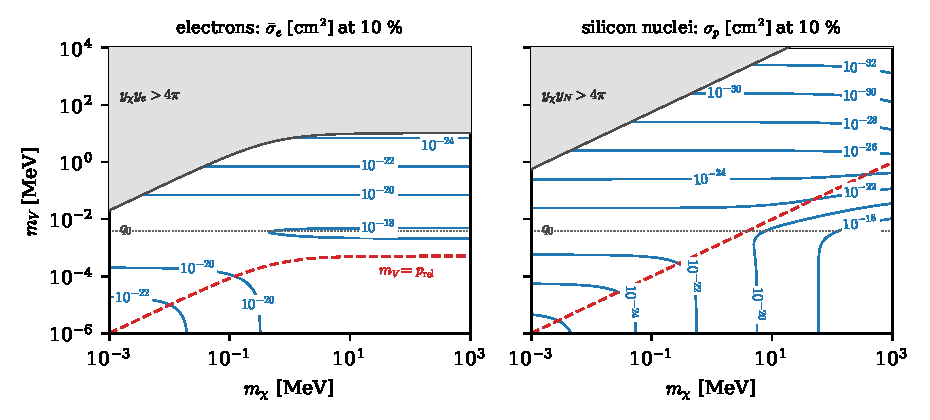
\includegraphics[width=\linewidth]{figures/ch08/limit8_2a.pdf}
\captionof{figure}{Cross-section at which $|\delta_{\mathrm{Born}}|$ of \cref{eq:8.2-born} reaches 0.1, against $\mchi$ and $m_V$, at $v = 10^{-3}$. Left: electrons, $\sigmae$ with the form factor normalized at $q_0 = \alpha m_e$ (\cref{eq:1.4-yukawa-sigma}). Right: silicon nuclei, coherent ($A = 28$), $\sigma_p$ normalized in the same way. With the coupling fixed by the cross-section, $\mchi$ enters only through $p_{\mathrm{rel}} = \mu_{\chi T}v$ (dashed, $m_V = p_{\mathrm{rel}}$; dotted, $m_V = q_0$). Gray: the \SI{10}{\percent} point needs $y_\chi y_e$ or $y_\chi y_N$ above $4\pi$, which happens for $m_V + p_{\mathrm{rel}} > 20A\mu_{\chi T}$ ($A = 1$ for electrons). At $\sigmae = \SI{e-37}{cm^2}$ and $\sigma_p = \SI{e-40}{cm^2}$ the largest correction in the plot is $4.5\times10^{-5}$ and $8.0\times10^{-5}$, at $m_V = \SI{10}{GeV}$. With perturbative couplings, \SI{10}{\percent} needs $\sigmae \ge \SI{4.9e-25}{cm^2}$ (at $m_V \approx \SI{10}{MeV}$) and $\sigma_p \ge \SI{1.6e-34}{cm^2}$ (at $\mchi = \SI{1}{GeV}$, $m_V = \SI{10}{GeV}$).}\label{fig:8-born-limit}
\par}
\smallskip
A correction of order one needs couplings near $4\pi$ with $m_V \lesssim 20A\mu_{\chi T}$, where the attractive potential binds and the cross-section has resonances that only the full partial-wave solution describes.
\end{limitbox}

\subsection{Absorption of a bosonic field}\label{sec:8.2-absorption}

A boson $\phi$ of mass $m_\phi$ that is absorbed leaves nothing behind, and its whole energy and momentum go into the target. By \cref{sec:8.1-absorption} its coupling is linear in the field and turns each target bilinear into a row at $\vect{q} = \vect{p}_\phi$. We write the coefficient of row $a$ per unit field amplitude as $g^\phi_a$, so that for the scalar of \cref{eq:8.1-scalar}, $g^\phi_{n_e} = -g_{\phi ee}$ and $g^\phi_{\mathcal{T}_e} = g_{\phi ee}/m_e$. For a vector field the polarization vector of the absorbed quantum sits inside $g^\phi_a$. Quantize the field in the box, with quanta of energy $\omega_\phi = m_\phi(1 + v^2/2)$. The matrix element that removes one quantum from a mode with $N_\phi$ quanta is $\sqrt{N_\phi/2\omega_\phi \Vol}\,\sum_bg^\phi_b\langle f|O_b(\vect{p}_\phi)|i\rangle$, and the golden rule, summed over $f$ and averaged over $i$, gives the response matrix again (\cref{app:D.25}). Per absorbed particle,
\begin{keyresult}[Master rate formula: absorption]
\begin{equation}
  \begin{gathered}
  \varGamma_{\mathrm{abs}} = \frac{1}{2\omega_\phi}\sum_{a,b}\underbrace{g^{\phi\,*}_a\,g^\phi_b}_{\text{coupling}}\,\underbrace{S_{ab}(\vect{p}_\phi,\omega_\phi)}_{\text{target}}, \\
  \varGamma_{\mathrm{net}} = (1 - \ee^{-\beta\omega_\phi})\,\varGamma_{\mathrm{abs}} = -\frac{1}{\omega_\phi}\,\Imag\sum_{a,b}g^{\phi\,*}_a\,g^\phi_b\,R_{ab}(\vect{p}_\phi,\omega_\phi) ,
  \end{gathered}
  \label{eq:8.2-abs}
\end{equation}
with $\omega_\phi \simeq m_\phi$. The event rate per unit target mass is $(\rho_\chi/m_\phi\rho_T)\langle\varGamma_{\mathrm{abs}}\rangle$, averaged over the directions and magnitudes of $\vect{p}_\phi = m_\phi\vect{v}$ with $f_\chi$.
\end{keyresult}
\noindent The absorption rate is the scattering formula evaluated at a single point, with $\mathfrak{D}_{ab}$ replaced by $g^{\phi\,*}_ag^\phi_b/2\omega_\phi$. The factor $1/2\omega_\phi$ is the relativistic normalization of one quantum. The number of quanta per unit volume, $\rho_\chi/m_\phi$, sets the event rate, not their flux: the speed of the dark matter enters only through the small momentum $\vect{p}_\phi$, as \cref{sec:2.1} found for a classical field.

The two rates in \cref{eq:8.2-abs} answer different questions. $\varGamma_{\mathrm{abs}}$ counts the quanta the target absorbs, each depositing $\omega_\phi$, and it is what a detector records. The field also stimulates the target to emit quanta into the occupied modes, at the rate $\ee^{-\beta\omega_\phi}\varGamma_{\mathrm{abs}}$ by detailed balance, and such an event takes energy out of the target. $\varGamma_{\mathrm{net}}$ is the difference, the rate at which the field loses quanta, and the fluctuation--dissipation theorem \cref{eq:4.2-fdt} writes it through the imaginary part of the response. That is the form in which Mitridate and collaborators state absorption, as the imaginary part of the self-energy of $\phi$, $\varGamma = -\Imag\Pi_{\phi\phi}/\omega$~\cite[Eqs.~(20)--(22)]{mitridate2021dark}, with $\Pi_{\phi\phi} = \sum_{ab}g^{\phi\,*}_ag^\phi_bR_{ab}$ in our normalization. For $\omega_\phi$ of an eV in a detector at \SI{10}{mK}, however, $\ee^{-\beta\omega_\phi}$ is zero for every purpose, and the two rates coincide.

The number of quanta in a volume $(1/m_\phi v)^3$ is $\rho_\chi/(m_\phi^4v^3)$, which exceeds one for $m_\phi$ below about \SI{7}{eV} at $v = 10^{-3}$, and grows as $m_\phi^{-4}$ below. Lighter bosons form a classical field rather than a gas of particles. The quantized calculation still applies, because the rate is linear in $N_\phi$ and the difference between $N_\phi$ and $N_\phi + 1$ in the emission matrix element, the spontaneous emission that a classical field lacks (\cref{sec:2.1}), is negligible. The same rate also follows from the classical field directly. Its amplitude is a sum of many modes with random phases, and by the central limit theorem it is a Gaussian random field. Averaging the transition probability over this Gaussian ensemble, the \emph{Gaussian field average}, removes the cross terms between different modes and leaves $\langle|\phi_{\vect{k}}|^2\rangle$ for each mode, which the energy density fixes; \cref{app:D.25} shows that the result is \cref{eq:8.2-abs} term by term.

The ensemble average needs an observation time long compared with the shorter of the coherence time $t_{\mathrm{coh}}$ of the field, of order $1/m_\phi v_0^2$, about \SI{1}{ns} at $m_\phi = \SI{1}{eV}$, and the inverse width of the target's response; a single record reproduces it only when it is also long compared with $t_{\mathrm{coh}}$. When both times exceed the record, for a field of neV mass or below acting on a sharp resonance such as a nuclear spin, the field drives the target coherently. The transition amplitude rather than the probability then grows linearly in time, and the golden rule gives way to the coherent classical-field treatment of \cref{sec:14.6}.

\Cref{eq:8.2-abs} reduces exactly to the dark-photon rate \cref{eq:1.4-dp-abs}. A dark photon at rest couples to the current of the electrons with strength $\zeta e$ times its polarization $\hat{\vect{e}}$ (\cref{sec:8.1-absorption}), and the only row is $\hat{\vect{e}}\cdot\vect{j}_e$, with $g^\phi = \zeta e$. With the proper current response $\tilde R^{\mathrm{T}}_{jj}$ of \cref{sec:4.4}, \cref{eq:8.2-abs} gives $\varGamma_{\mathrm{net}} = -(\zeta^2e^2/m_\phi)\Imag\tilde R^{\mathrm{T}}_{jj}(m_\phi)$. The diamagnetic term of the current is real and does not contribute. By the transverse dielectric function of \cref{sec:4.4}, $\varepsilon_2 = -(e^2/\omega^2)\Imag\tilde R^{\mathrm{T}}_{jj}$, and with $\sigma_1 = \omega\varepsilon_2$ (\cref{eq:4.4-sigma}) the rate is $\zeta^2\sigma_1(m_\phi)$, the same for every polarization in a cubic crystal (\cref{eq:4.4-ET}). The full response also contains the chain in which the induced current radiates an ordinary photon that the target absorbs again. Summing it, \cref{app:D.25} shows that it turns $\zeta^2$ into $\zeta_{\mathrm{eff}}^2$ of \cref{sec:1.4}. Multiplying by $\rho_\chi/m_\phi\rho_T$ gives \cref{eq:1.4-dp-abs}.

Fermionic absorption (\cref{sec:8.1-absorption}) fits the same formula. The dark matter disappears and a light fermion $\tilde\nu$ leaves with momentum $\vect{p} - \vect{q}$. The sum over final dark-matter momenta that produced \cref{eq:8.2-rate} becomes the sum over the momenta of $\tilde\nu$, and energy conservation sets $\omega$ to \cref{eq:8.1-omega}, which is $\mchi - q$ for a massless $\tilde\nu$. The rows and $S_{ab}$ are those of scattering, now sampled along a line at $q \approx \mchi$. Only $\mathfrak{D}_{ab}$ changes: the spinors of the relativistic $\tilde\nu$ enter it with relativistic normalization, which \cref{sec:10.9} constructs.

\subsection{Negative energies and exothermic dark matter}\label{sec:8.2-exothermic}

The master formula holds for either sign of $\omega$. The kinematics of scattering allows it to be negative: a dark-matter particle that moves against $\vect{q}$, or that recoils with more kinetic energy than it brings, gains energy, $\omega_{\vect{q}} < 0$. Whether such a transfer happens is decided by the target alone. At $T = 0$ the target starts in its ground state, $S_{ab}(\vect{q},\omega)$ vanishes for $\omega < 0$, and the half-plane below the axis in \cref{fig:8-plane} is closed. A warm target opens it, with the weight fixed by detailed balance. In matrix form, $S_{ab}(-\vect{q},-\omega) = \ee^{-\beta\omega}S_{ba}(\vect{q},\omega)$ (\cref{sec:4.2}), so a transfer of $\omega < 0$ is suppressed relative to the reverse one by $\ee^{-\beta|\omega|}$, the Boltzmann factor of the excitation the target gives up. For an electronic excitation across the gap of silicon, this factor is smaller than any power of the temperature, and an expansion in the phonon occupations (the thermal order $n_T$ of \cref{sec:8.5}) drops it at every order. For a phonon it is the occupation $n_{\vect{Q}\nu}$ itself: the negative-$\omega$ part of a one-phonon rate is proportional to $n_{\vect{Q}\nu}$, of first order in the occupations. The same holds for absorption, whose emission partner sits at the point $(-\vect{p}_\phi, -\omega_\phi)$.

Exothermic dark matter does something different: it does not reweight the band, it moves it. A particle that arrives in an excited state and leaves in the lower one, with $\Delta_\chi < 0$, adds $|\Delta_\chi|$ to every $\omega_{\vect{q}}$ of \cref{eq:1.3-omegaq}. The band of allowed $(\vect{q}, \omega)$ shifts up by $|\Delta_\chi|$, reaches $q \to 0$ at $\omega = |\Delta_\chi|$, and there looks like the absorption of a boson of mass $|\Delta_\chi|$, with $\vect{q}$ set by the velocity rather than fixed at $m_\phi\vect{v}$ (\cref{fig:8-plane}). Since the energy now comes from the dark matter, the target needs no temperature, and the response is sampled at positive $\omega$ even for the slowest particles. An endothermic splitting, $\Delta_\chi > 0$, shifts the band down, and part of it can then be reached only with energy taken from a warm target.

Detailed balance ties the two directions of each transition, for the dark matter as well as for the target. Let $\vect{p}$ and $\vect{p}'$ be two dark-matter states, of any masses, and $\omega = E(\vect{p}) - E(\vect{p}')$ the energy that the transition $\vect{p} \to \vect{p}'$ deposits. Then, for unpolarized dark-matter states of equal spin,
\begin{equation}
  \varGamma(\vect{p}' \to \vect{p}) = \ee^{-\beta\omega}\,\varGamma(\vect{p} \to \vect{p}') ,
  \label{eq:8.2-db}
\end{equation}
for the rate into one final momentum (\cref{app:D.25}). The reverse transition is driven by the conjugated interaction, which exchanges $\mathfrak{D}_{ab}$ for $\mathfrak{D}_{ba}$ and $O_b$ for $O_b^\dagger$, and the two exchanges cancel in the contraction; what remains is the ratio of the Gibbs weights of the two target states. The down-scattering of an exothermic particle, $\chi_2 \to \chi_1$, and the up-scattering $\chi_1 \to \chi_2$ that a warm target can drive are therefore one process read in two directions. A population of dark matter in contact with the target for long enough would relax to the temperature of the target.

\begin{figure}[tbp]
  \centering
  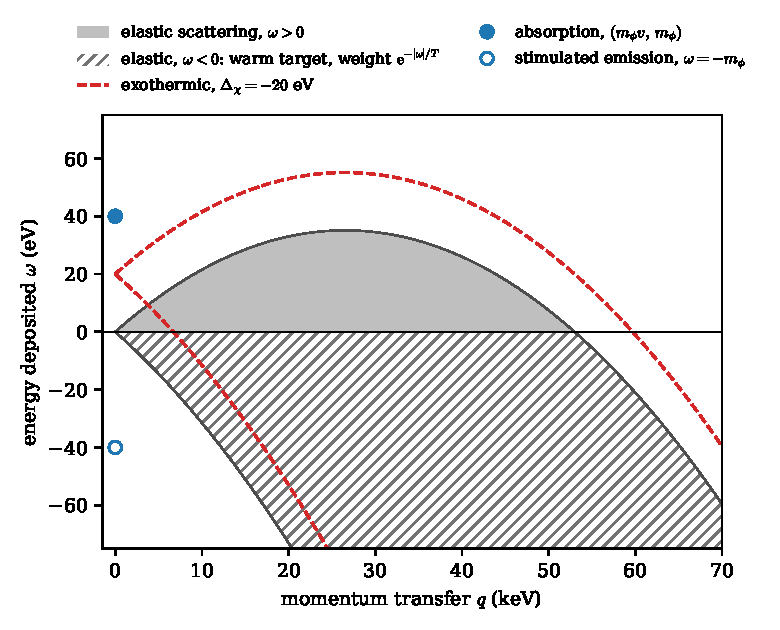
\includegraphics[width=0.9\linewidth]{figures/ch08/fig8_1.pdf}
  \caption{Where the master rate formula samples the response, in the plane of momentum transfer $q$ and energy deposited $\omega$, for $\mchi = \SI{10}{MeV}$ and speeds up to $v_{\mathrm{max}} = 2.650\times10^{-3}$. Elastic scattering reaches the band $-qv_{\mathrm{max}} - q^2/2\mchi \le \omega \le qv_{\mathrm{max}} - q^2/2\mchi$, the extreme values of $\omega_{\vect{q}}$ over all directions of $\vect{v}$. Its upper part (gray, $\omega > 0$, maximum \SI{35}{eV} at $q = \mchi v_{\mathrm{max}} = \SI{26.5}{keV}$) is open at any temperature. Its lower part (hatched, $\omega < 0$) is open only for a target at $T > 0$, with weight $\ee^{-|\omega|/T}$ relative to the reverse transfer. Exothermic dark matter with $\Delta_\chi = \SI{-20}{eV}$ shifts the band up by $|\Delta_\chi|$ (dashed). Absorption of a boson of mass $m_\phi = \SI{40}{eV}$ is a point at $q = m_\phi v \approx \SI{40}{meV}$, $\omega = m_\phi$ (filled circle); stimulated emission into the occupied field is the point $\omega = -m_\phi$ (open circle). Fermionic absorption with a massless outgoing fermion, $\omega = \mchi - q$, is a line at $q \approx \mchi$, far to the right.}
  \label{fig:8-plane}
\end{figure}

\subsection{Conditions for off-diagonal terms}\label{sec:8.2-cross}

The off-diagonal terms of the contraction are the part of a rate that no single-operator calculation contains. They need two things at once. The dark-matter side must couple two rows with a nonzero product $\mathfrak{D}_{ab}$, and the target must correlate the same two rows, $S_{ab} \neq 0$. Each factor vanishes for a reason of symmetry in the commonest cases. On the dark-matter side, a coefficient linear in $\vect{S}_\chi$ never interferes with one that is independent of it (\cref{sec:8.1}). On the target side, the density and the spin density of a target without magnetic order are uncorrelated, since $\Tr\boldsymbol{\sigma} = 0$. The worked example takes a target with magnetic order and a coupling that survives the trace over the dark-matter spin.

\begin{workedexample}{Density and spin couplings in a polarized electron gas}\label{we:8-cross}
Take the free electron gas at the valence density of silicon, $\nd_e = \SI{2.00e23}{cm^{-3}}$, fully polarized along $\hat{\vect{z}}$ by a uniform exchange field strong enough to lift the minority band above the Fermi level, a toy half-metal. All electrons have $S_z = +\frac12$ and fill one Fermi sphere of radius $k_{\mathrm{F}\uparrow} = 2^{1/3}k_{\mathrm{F}} = \SI{4.50}{keV}$, with $v_{\mathrm{F}\uparrow} = 8.80\times10^{-3}$ and $E_{\mathrm{F}\uparrow} = \SI{19.8}{eV}$; the exchange splitting must exceed $E_{\mathrm{F}\uparrow}$. We work at $T = 0$ with two rows, the density $n_e$ and the spin density $s^z_e$ of \cref{eq:8.1-rows}.

The Hamiltonian conserves the spin of each electron, so every state that $n_e$ or $s^z_e$ reaches from the ground state has all spins up, and on those states $s^z_e(\vect{q}) = \frac12 n_e(\vect{q})$ exactly. The response matrix is then
\begin{equation*}
  \begin{pmatrix} S_{nn} & S_{ns} \\ S_{sn} & S_{ss} \end{pmatrix} = S_\uparrow(\vect{q},\omega)\begin{pmatrix} 1 & \frac12 \\ \frac12 & \frac14 \end{pmatrix} ,
\end{equation*}
with $S_\uparrow$ the structure factor of one spin, half of \cref{eq:4.2-gas} with $k_{\mathrm{F}} \to k_{\mathrm{F}\uparrow}$. Its determinant vanishes: the two rows are one operator, and the matrix saturates the bound \cref{eq:4.2-positivity}. At $q = q_0 = \SI{3.73}{keV}$ and $\omega = \SI{5}{eV}$ we are in the linear region of the sphere, below $qv_{\mathrm{F}\uparrow} - q^2/2m_e = \SI{19.2}{eV}$, and $S_\uparrow = m_e^2\omega/2\pi q = \SI{5.57e7}{eV^2}$, half of the unpolarized gas at the same density.

For potentials $\tilde V_n$ and $\tilde V_s$ on the two rows, real and without dark-matter spin, the contraction is
\begin{equation*}
  \tilde V_n^2S_{nn} + 2\tilde V_n\tilde V_sS_{ns} + \tilde V_s^2S_{ss} = S_\uparrow\bigl(\tilde V_n + \tfrac12\tilde V_s\bigr)^2 .
\end{equation*}
Every electron carries $S_z = \frac12$, so a coupling to the spin acts as an extra density potential and adds to it in the amplitude. The sum of the two single-operator rates is $S_\uparrow(\tilde V_n^2 + \tilde V_s^2/4)$. It misses the term $\tilde V_n\tilde V_sS_\uparrow$, which is first order in the weaker coupling, and at $\tilde V_s = -2\tilde V_n$, where the true rate vanishes, it is wrong by the whole of $2\tilde V_n^2S_\uparrow$.

Which models produce such a $\tilde V_s$? The standard pair $\mathcal{O}_1$ and $\mathcal{O}_4 = \vect{S}_\chi\cdot\vect{S}_e$ does not: $\tilde V_s = c_4^{(e)}\vect{S}_\chi$, and the trace over the unpolarized dark-matter spin removes the cross term. A spin coupling free of $\vect{S}_\chi$ is $\mathcal{O}_7 = \vect{S}_e\cdot\vect{v}^\perp$, which reduces to $\bar{\vect{v}}_\chi\cdot\vect{s}_e - \mathcal{J}^{\alpha\alpha}_e$ (\cref{tab:8-operators}). No standard model produces $\mathcal{O}_7$ at leading order (\cref{sec:8.1}); we take it as the simplest spin coupling that survives the trace. Take it together with $\mathcal{O}_1$, with coefficients $c_1$ and $c_7$. The rows $s^x_e$, $s^y_e$, $\mathcal{J}^{xx}_e$ and $\mathcal{J}^{yy}_e$ flip the spin and reach states orthogonal to those of $n_e$, so the terms of first order in $c_7$ are
\begin{equation*}
  2c_1c_7\bigl[\bar v_{\chi,z}\,S_{ns} - S_{n\mathcal{J}}\bigr], \qquad
  S_{n\mathcal{J}} = \tfrac12\Bigl\langle\frac{(2\vect{k} + \vect{q})_z}{2m_e}\Bigr\rangle S_\uparrow ,
\end{equation*}
since the element of $\mathcal{J}^{zz}_e$ between $\vect{k}$ and $\vect{k} + \vect{q}$ is $\frac12(2\vect{k} + \vect{q})_z/2m_e$, and the brackets average over the pairs at this $(\vect{q},\omega)$. Since the pairs fill an annulus symmetric about $\vect{q}$ (\cref{we:8-O2}), the transverse part of $\vect{k}$ averages away, and $(2\vect{k} + \vect{q})\cdot\hat{\vect{q}}/2m_e = \omega/q$ for every pair. As a result, $S_{n\mathcal{J}} = \frac12(\omega/q)\hat q_zS_\uparrow$. On the dark-matter side, $\hat{\vect{q}}\cdot\bar{\vect{v}}_\chi = \omega/q$ for elastic scattering, so $\bar v_{\chi,z} = (\omega/q)\hat q_z + \vect{v}_{\mathrm{T}}\cdot\hat{\vect{z}}$, with $\vect{v}_{\mathrm{T}}$ the part of $\vect{v}$ transverse to $\vect{q}$. The longitudinal parts cancel, as \cref{eq:8.1-transverse} requires, and the integrand of \cref{eq:8.2-rate} becomes
\begin{equation*}
  c_1^2\,S_\uparrow + c_1c_7\,(\vect{v}_{\mathrm{T}}\cdot\hat{\vect{z}})\,S_\uparrow + O(c_7^2) .
\end{equation*}
For the dark matter of \cref{we:8-O2}, $\mchi = \SI{100}{MeV}$ and $v = 2.0\times10^{-3}$, $\vmin = 1.36\times10^{-3}$ and $v_{\mathrm{T}} = 1.47\times10^{-3}$. With $\vect{v}_{\mathrm{T}}$ along the magnetization, the cross term is $1.5\times10^{-3}\,c_7/c_1$ of the $\mathcal{O}_1$ rate. The rate of $\mathcal{O}_7$ alone is second order in $c_7$ and quadratic in the velocities. Its squared matrix elements, summed over the final spin, are $|\vect{v}^\perp|^2/4 \le (v_{\mathrm{max}} + v_{\mathrm{F}\uparrow} + q/2m_e)^2/4 = 5.7\times10^{-5}$, and its structure factors are at most $S_\uparrow$ and $m_ek_{\mathrm{F}\uparrow}^2/4\pi q = 4.0\,S_\uparrow$, the second for spin flips into the empty minority band, which an exchange splitting above $E_{\mathrm{F}\uparrow} + \omega$ closes; the bound is generous. At $c_7 = c_1$ the cross term is therefore at least five times the rate of $\mathcal{O}_7$ alone.

The cross term is odd in $\vect{v}_{\mathrm{T}}$. At fixed $\vect{q}$ the halo integral runs over the velocities with $\hat{\vect{q}}\cdot\vect{v} = \vmin$, and for the laboratory Maxwellian $f_\chi \propto \ee^{-|\vect{v} + \vect{v}_{\mathrm{E}}|^2/v_0^2}$ of \cref{app:A.8} the exponent splits into a longitudinal and a transverse Gaussian. Apart from the escape cut, the transverse Gaussian is centered on $-\vect{v}_{\mathrm{E},\mathrm{T}}$, the part of $-\vect{v}_{\mathrm{E}}$ transverse to $\vect{q}$, and the averaged cross term is $-c_1c_7\,(\vect{v}_{\mathrm{E},\mathrm{T}}\cdot\hat{\vect{z}})\,S_\uparrow$, at most $8.4\times10^{-4}\,c_7/c_1$ of the $\mathcal{O}_1$ rate for $|\vect{v}_{\mathrm{E}}| = \SI{250.5}{km.s^{-1}}$. It vanishes for an isotropic halo, follows the angle between the magnetization and the dark-matter wind, and changes sign when the magnetization is reversed.

A partially polarized gas has two spheres and $S_{ns} = \frac12(S_\uparrow - S_\downarrow)$. In the linear region, however, the structure factor of one spin, $m_e^2\omega/2\pi q$, does not depend on the radius of its sphere, and $S_{ns}$ vanishes there even though the gas is magnetized. At a polarization of 0.5 and $q = q_0$, $S_{ns} = 0$ at \SI{5}{eV}; at \SI{10}{eV}, where the minority sphere has left its linear region (its edge is at \SI{7.07}{eV}), $S_{ns}/S_{nn} = 0.068$.
\end{workedexample}

A cross term needs a coupling and a target that break the same symmetry, here time reversal, and when both do, it enters the rate at first order in the weaker coupling, where each single-operator rate enters at second order. How large it can be is fixed by positivity, and the polarized gas reaches the limit; \cref{sec:8.3} derives the bound together with the other relations that hold for every target.

\section{Exact relations}\label{sec:8.3}

A computed response of silicon can be wrong in ways that no convergence test reveals. Take an electron--nucleus interference spectrum that keeps one sign, an energy-weighted spectrum that counts thirteen electrons per atom, or a coupling proportional to mass that excites optical phonons at vanishing momentum transfer. Each is an error, whatever the method and however well converged, because each violates a relation that holds for every target. \Cref{sec:4.2,sec:4.3} derived the first of these relations: detailed balance, the positivity of the response matrix, the fluctuation--dissipation theorem, the Kramers--Kronig relations and the f-sum rule of every species. The multi-operator rate of \cref{sec:8.2} needs three more: an interference bound, higher moments and a Ward identity. Positivity limits how strongly two couplings can interfere. The higher frequency moments of the response matrix are fixed by commutators, and the third moment of the electron--nucleus interference turns out to be set by the electron density at the nuclei. Translation invariance links the densities of all species to the momentum density, and as a result a coupling proportional to mass can only make sound at long wavelengths. None of these relations depends on an approximation to the target, so a response that violates one is wrong, not merely truncated.

\subsection{Interference of two couplings}\label{sec:8.3-bound}

In the polarized electron gas of \cref{we:8-cross} the rate of a density and a spin coupling together was $S_\uparrow(\tilde V_n + \frac12\tilde V_s)^2$, which can be anything from zero to twice the sum of the two single-operator rates. How far can a cross term go in general? Split the rows of \cref{eq:8.2-rate} into two groups, $A$ and $B$, for instance the electron rows and the nuclear rows of a dark photon, or the density and the current rows of \cref{sec:8.1}. The rate is then
\begin{equation*}
  \varGamma = \varGamma_A + \varGamma_{AB} + \varGamma_B ,
\end{equation*}
where $\varGamma_A$ and $\varGamma_B$ keep only the terms with both indices in one group, the rates of each group alone, and the cross term $\varGamma_{AB}$ collects the terms with one index in each, $2\Real\sum_{a\in A,b\in B}\mathfrak{D}_{ab}S_{ab}$ under the integral.

The bound follows from a family of models. Multiply every coupling of group $B$ by a real number $\lambda$. Each element $\mathfrak{D}_{ab}$ is multiplied by $\lambda$ once for every index in $B$, which is $\mathfrak{D}$ multiplied on both sides by a real diagonal matrix, so the tensor is still Hermitian and positive semidefinite. Its contraction with the positive semidefinite $S_{ab}$ of \cref{eq:4.2-positivity} is therefore never negative, at every $(\vect{q},\omega)$ and for every velocity. So is the rate after any integration over $\vect{q}$, $\omega$ and the halo:
\begin{equation*}
  \varGamma(\lambda) = \varGamma_A + \lambda\,\varGamma_{AB} + \lambda^2\,\varGamma_B \ge 0 \qquad \text{for every real } \lambda .
\end{equation*}
A quadratic that never goes negative has a discriminant that is not positive, $\varGamma_{AB}^2 \le 4\varGamma_A\varGamma_B$.
\begin{keyresult}[Interference bound]
For any two groups of rows, any target and any dark-matter model,
\begin{equation}
  |\varGamma_{AB}| \le 2\,(\varGamma_A\varGamma_B)^{1/2} , \qquad\text{equivalently}\qquad
  \bigl(\varGamma_A^{1/2} - \varGamma_B^{1/2}\bigr)^2 \le \varGamma \le \bigl(\varGamma_A^{1/2} + \varGamma_B^{1/2}\bigr)^2 .
  \label{eq:8.3-bound}
\end{equation}
The cross term is at most twice the geometric mean of the separate rates. The bound holds pointwise in $(\vect{q},\omega)$, for the spectrum $\dd\mathcal{R}/\dd\omega$ in any bin, and for the total rate.
\end{keyresult}
\noindent For one row in each group the pointwise statement is the Cauchy--Schwarz inequality $|S_{ab}|^2 \le S_{aa}S_{bb}$ of \cref{eq:4.2-positivity} combined with $|\mathfrak{D}_{ab}|^2 \le \mathfrak{D}_{aa}\mathfrak{D}_{bb}$ from \cref{eq:8.1-D}, and the integrated statement then follows from the Cauchy--Schwarz inequality for integrals, $\int(xy)^{1/2} \le (\int x\int y)^{1/2}$. The argument through $\lambda$ gives both at once, and for blocks of any size.

The bound is reached when both matrices have rank one on the two groups and their phases line up, as in the polarized gas: there $S_{ns}^2 = S_{nn}S_{ss}$, and at $\tilde V_s = -2\tilde V_n$ the rate sits on the lower edge of \cref{eq:8.3-bound}, zero. The bound is not an estimate. For an unpolarized target and couplings that are blind to the dark-matter spin, the cross terms between density and spin vanish by symmetry (\cref{sec:8.2-cross}), far inside the band. Its use is to put a rigorous band on a rate whose interference term has not been computed: writing $r = \varGamma_B/\varGamma_A$, the total lies between $(\sqrt r - 1)^2$ and $(\sqrt r + 1)^2$ times $\varGamma_A$. The same inequality bounds the Migdal interference, $|S_{e\kappa}|^2 \le S_{ee}S_{\kappa\kappa}$, and enters the nuisance parameters of \cref{sec:8.8} as a constraint.

\subsection{Moment matrices}\label{sec:8.3-moments}

The f-sum rule fixed the first frequency moment of every density by a double commutator (\cref{eq:4.3-firstmoment,eq:4.3-species}). Higher moments weight the spectrum toward high energies, and they are where an approximation to the core electrons or to the electron--nucleus interaction shows up. We collect them into matrices,
\begin{equation}
  \mathscr{M}^k_{ab}(\vect{q}) \equiv \int_{-\infty}^{\infty}\frac{\dd\omega}{2\pi}\;\omega^k\bigl[S_{ab}(\vect{q},\omega) + S_{ba}(-\vect{q},\omega)\bigr]
  = \frac{1}{\Vol}\Bigl\langle\bigl[O_a(\vect{q})^\dagger,\,[H, O_b(\vect{q})]_k\bigr]_{\mp}\Bigr\rangle ,
  \label{eq:8.3-moments}
\end{equation}
for operators with $O(-\vect{q}) = O(\vect{q})^\dagger$ and any stationary state, where $[H, O]_k$ is $O$ commuted $k$ times with $H$, as in \cref{sec:4.3}, and $[X, Y]_\mp$ is the commutator $XY - YX$ for odd $k$ and the anticommutator $XY + YX$ for even $k$. The derivation of \cref{eq:4.3-moments} goes through unchanged. The term $O_a^\dagger[H, O_b]_k$ gives the $k$-th moment of $VS_{ab}(\vect{q},\omega)/2\pi$, the term $[H, O_b]_kO_a^\dagger$ gives $(-1)^k$ times that of $VS_{ba}(-\vect{q},\omega)/2\pi$, and the sign of the bracket makes the two add for every $k$. For $k = 1$ this is \cref{eq:4.3-firstmoment}, so $\mathscr{M}^1$ is the first-moment matrix of \cref{sec:4.3}. Since $S_{ab}$ has the units of $\mathrm{eV}^2$ for densities, $\mathscr{M}^k$ has those of $\mathrm{eV}^{k+3}$.

The odd and the even moments carry different information. An odd moment is a commutator. It needs only the algebra of $H$ and equal-time averages of simpler operators, and for the densities of electrons and nuclei the first one is a number, \cref{eq:4.3-species}. An even moment is an equal-time correlation function. On the diagonal, with $X = [H, O_a]_{k/2}$, it reads $\Vol^{-1}\langle X^\dagger X + XX^\dagger\rangle$; for instance $\mathscr{M}^0_{ee} = 2\nd_eS^{\mathrm{st}}$ for a target with inversion symmetry, by \cref{eq:4.2-static}. It depends on the state, its temperature and its correlations, but no dynamics is needed to compute it, which is why the moments of the nuclear self response can be taken from a static path-integral simulation (\cref{app:E.19}). In the same way as for $k = 1$ in \cref{sec:4.3}, an odd $\mathscr{M}^k$ is the coefficient of $z^{-(k+1)}$ in the expansion of $R_{ab}(\vect{q}, z)$ at large $z$ (\cref{app:D.26}).

Positivity constrains the moments among themselves. The spectral weight of one row, summed over $\pm\vect{q}$, is never negative. It defines a positive measure on the real line, and its moments $\mathscr{M}^k_{aa}$ form a Hankel matrix, with elements $\mathscr{M}^{i+j}_{aa}$, that is positive semidefinite:
\begin{equation}
  \sum_{i,j=0}^{n}x_i\,x_j\,\mathscr{M}^{i+j}_{aa} = \int\frac{\dd\omega}{2\pi}\Bigl(\sum_ix_i\omega^i\Bigr)^2\bigl[S_{aa}(\vect{q},\omega) + S_{aa}(-\vect{q},\omega)\bigr] \ge 0 .
  \label{eq:8.3-hankel}
\end{equation}
The smallest case is $(\mathscr{M}^1_{aa})^2 \le \mathscr{M}^0_{aa}\mathscr{M}^2_{aa}$. At $T = 0$ the measure lives on $\omega \ge 0$, and the shifted matrix $\mathscr{M}^{i+j+1}_{aa}$ is positive semidefinite too, which gives for instance $(\mathscr{M}^2_{aa})^2 \le \mathscr{M}^1_{aa}\mathscr{M}^3_{aa}$. A spectrum is determined, within a band that these inequalities make precise, by its first few moments, the Markov--Krein band of \cref{sec:11.5}.

How many moments exist? For electrons and point nuclei with Coulomb interactions, $\mathscr{M}^3$ is finite and $\mathscr{M}^4$ is not. The fourth moment of a density is the equal-time average of $|[H,[H,n_s]]|^2$, and $[H,[H,n_s]]$ contains the force on each particle (\cref{app:D.26}). The mean square of the Coulomb force between an electron and a nucleus, $\int\dd^3y\,\nd(\vect{y})\,(Z_\kappa\alpha/y^2)^2$ with $\nd$ finite at the nucleus, diverges as $\int\dd y/y^2$. The spectrum shows the same thing at large $\omega$. The oscillator strength of the hydrogen continuum falls as $\omega^{-7/2}$ (\cref{we:4-trk}), and at small $q$, where $S \propto q^2\,\omega^{-1}\dd f^{\mathrm{osc}}/\dd\omega$, the structure factor falls as $\omega^{-9/2}$: $\omega^3S$ is integrable and $\omega^4S$ is not. In the Born--Oppenheimer approximation, the order $n_B = 0$ of the expansion in the derivative coupling of \cref{sec:8.5}, the nuclei move on a smooth energy surface, and every moment of their self response is finite.

\subsection{The mixed third moment}\label{sec:8.3-third}

The first moment of the electron--nucleus interference vanishes, \cref{eq:4.3-species}, and at $T = 0$ the real part of $S_{e\kappa}$ must change sign along the energy axis. Which sign wins at high energy, where the Migdal effect and core excitations live? The third moment weights the spectrum by $\omega^3$ and answers the question.

The calculation takes three steps, written out in \cref{app:D.26}. First, in a stationary state the average of $[X, [H, Y]]$ equals that of $[[X, H], Y]$, since the average of a commutator with $H$ vanishes; this moves one commutator onto the electron density, $\mathscr{M}^3_{e\kappa} = \Vol^{-1}\langle[[n_e^\dagger, H], [H, [H, n_\kappa]]]\rangle$. Second, the continuity equations of the two species, \cref{eq:4.3-continuity} and its nuclear analogue, turn the two inner commutators into currents, $[n_e(\vect{q})^\dagger, H] = \vect{q}\cdot\vect{j}_e(\vect{q})^\dagger$ and $[H, n_\kappa(\vect{q})] = \vect{q}\cdot\vect{j}_\kappa(\vect{q})$. Third, the commutator of $H$ with the nuclear current contains the kinetic energy of the nuclei and the gradient of the potential energy at each nucleus, $\ii M_\kappa^{-1}\sum_{I\in\kappa}\ee^{\ii\vect{q}\cdot\vect{X}_I}\,\vect{q}\cdot\nabla_IU$, with $U$ the potential energy. The electron current commutes with every nuclear operator. It fails to commute only with the electron positions inside the force, and only the electron--nucleus Coulomb energy $\sum_{j,I}w_\kappa(\vect{r}_j - \vect{X}_I)$, $w_\kappa(\vect{y}) = -Z_\kappa\alpha/y$, depends on both. The electron--electron and nucleus--nucleus interactions, and every kinetic term, drop out. What is left involves one function, the mean electron density $\nd_e^{(\kappa)}(\vect{y})$ at the displacement $\vect{y}$ from a nucleus of species $\kappa$, averaged over the nuclei of that species and over their motion. Its value at $\vect{y} = 0$ is the contact density $\nd_e^{(\kappa)}$, the electron density at the nucleus, and far from the nucleus it averages to the mean density $\nd_e$.
\begin{keyresult}[Mixed electron--nucleus third moment]
For point nuclei, nonrelativistic electrons and local potentials, at any $\vect{q}$, temperature and coupling strength,
\begin{equation}
  \mathscr{M}^3_{e\kappa}(\vect{q}) = -\frac{\nd_\kappa}{m_eM_\kappa}\int\dd^3y\;\nd_e^{(\kappa)}(\vect{y})\,\ee^{-\ii\vect{q}\cdot\vect{y}}\,(\vect{q}\cdot\nabla)^2w_\kappa(\vect{y}) .
  \label{eq:8.3-M3}
\end{equation}
At sites of cubic symmetry, for $q$ small compared with the shortest reciprocal-lattice vector $G_{\mathrm{min}}$ but large compared with the inverse size of the sample,
\begin{equation}
  \mathscr{M}^3_{e\kappa}(\vect{q}) = -\frac{Z_\kappa e^2q^2\,\nd_\kappa}{3\,m_eM_\kappa}\bigl[\nd_e^{(\kappa)} + 2\nd_e\bigr] .
  \label{eq:8.3-M3lim}
\end{equation}
The high-frequency interference of electrons and nuclei is negative, and its weight is fixed by the electron density at the nuclei.
\end{keyresult}
\noindent The third moment of a single species is classical, and Puff wrote it for an interacting Bose fluid~\cite{puff1965application}. The two terms of the bracket have different origins, which the identity
\begin{equation*}
  (\vect{q}\cdot\nabla)^2\frac{1}{y} = -\frac{4\pi}{3}\,q^2\,\delta^3(\vect{y}) + q^2\,\frac{3(\hat{\vect{q}}\cdot\hat{\vect{y}})^2 - 1}{y^3}
\end{equation*}
makes visible. The contact part picks out the density at the nucleus and gives $\nd_e^{(\kappa)}/3$ at every $q$, with the phase $\ee^{-\ii\vect{q}\cdot\vect{y}}$ equal to one on its support. The quadrupolar part averages to zero against any density with cubic symmetry about the nucleus that varies on scales short compared with $1/q$, the core and the valence bonds alike. Against the uniform part of the density, however, it does not vanish. That integral is dominated by distances $y \sim 1/q$, where the phase matters, and since the kernel scales as $1/y^3$ it is independent of $q$; it contributes $2\nd_e/3$. It is the Coulomb field of the bare nucleus acting on the electrons of the whole crystal at distances $\sim 1/q$. The order of limits is the physical one: the sample is infinite at fixed $q$, and only then is $q$ small.

The sign has a simple reading. For an electron bound to a nucleus by a spring of constant $K$, \cref{eq:8.3-M3} gives $\mathscr{M}^3_{e\kappa} = -Kq^2/(m_eM_\kappa \Vol)$ at small $q$. The relative coordinate makes the sign obvious: in the mode in which the two particles oscillate against each other, at $\omega^2 = K(m_e^{-1} + M_\kappa^{-1})$, a displacement of one is accompanied by an opposite displacement of the other (\cref{app:D.26}). The Coulomb attraction is a spring whose stiffness, the curvature $\nabla^2w_\kappa = Z_\kappa e^2\delta^3(\vect{y})$, sits at the nucleus, and the contact density measures how much of the electron cloud feels it. Together with the vanishing first moment, the negative third moment says that the interference is positive at low energies, where the electrons follow the nucleus (\cref{sec:8.6}), and negative at high energies, where they are left behind. The positive part sits in the phonon final states, on the acoustic branch, at energies that vanish with $q$, and on the optical phonons, wherever the electrons move with the nuclei (\cref{sec:8.6}). Every electronic final state carries the negative interference $-(m_e/M_\kappa)|\langle f|n_e|0\rangle|^2$ at small $q$, as \cref{eq:8.3-boostward} below shows.

\Cref{eq:8.3-M3lim} has a limited range in $q$, and three regimes follow from the exact form, which \cref{app:D.26} writes as a sum over reciprocal-lattice vectors. For $q \ll G_{\mathrm{min}}$, \cref{eq:8.3-M3lim} holds. Its real part is corrected at relative order $(q/G_{\mathrm{min}})^2$ at every cubic site. At sites without inversion symmetry, such as the tetrahedral sites of silicon, there is also a correction of first order in $q/G_{\mathrm{min}}$. It is purely imaginary. It comes from the part of the density odd about the nucleus, whose Fourier components are imaginary, and it enters $\Imag\mathscr{M}^3_{e\kappa}$ alone. In silicon $G_{\mathrm{min}} = |\vect{G}_{111}| = \SI{3.95}{keV}$ (\cref{sec:3.1}). Once $q$ passes $G_{\mathrm{min}}$ the valence structure starts to matter, and the bracket depends on $q$, although the contact term still dominates. Once $q$ reaches the inverse size $1/a_{\mathrm{core}}$ of the innermost shell, the core itself is resolved: the quadrupolar kernel then acts on the density near the nucleus as on a uniform one, and the bracket climbs from $\nd_e^{(\kappa)}/3$ toward $\nd_e^{(\kappa)}$. For a density with spherical symmetry about the nucleus, which is exact for a free atom and a good approximation for the core in a cubic crystal, the angular integral of \cref{eq:8.3-M3} can be done once and for all (\cref{app:D.26}):
\begin{equation}
  \mathscr{M}^3_{e\kappa}(\vect{q}) = -\frac{Z_\kappa e^2q^2\,\nd_\kappa}{m_eM_\kappa}\Bigl[\frac{\nd_e^{(\kappa)}}{3} + 2\int_0^\infty\dd y\;\frac{\bar\nd_e^{(\kappa)}(y)\,j_2(qy)}{y}\Bigr] ,
  \label{eq:8.3-M3sph}
\end{equation}
with $\bar\nd_e^{(\kappa)}(y)$ the spherically averaged density at distance $y$ from the nucleus and $j_2$ the spherical Bessel function of order two. Since $\int_0^\infty\dd x\,j_2(x)/x = 1/3$, a density that is uniform over the range $y \sim 1/q$ contributes $2/3$ of its value through the integral. This is the origin of the $2\nd_e/3$ of the small-$q$ limit.

The contact density is a material quantity in its own right, and it is computed from all-electron densities. Pseudopotential calculations replace the cores and cannot supply it; the projector-augmented-wave reconstruction or a full-potential code restores the density near the nucleus. The spherical atomic part comes from a calculation of the free atom, and the crystal adds a small anisotropy of the valence (\cref{app:E.17}). Relativity changes the density at the nucleus more than anything else. For a finite nucleus it raises the contact density by about \SI{8}{\percent} in silicon, an effect that grows roughly as $(Z\alpha)^2$ in heavier atoms and that \cref{sec:12.5} adds to \cref{eq:8.3-M3lim}.

\begin{workedexample}{The mixed third moment of silicon}\label{we:8-third}
We evaluate \cref{eq:8.3-M3sph} for silicon at $q = \SI{10}{keV}$, a typical momentum transfer for the Migdal effect. For the density we take the free atom in its ground state from an all-electron Hartree--Fock calculation, nonrelativistic and with a point nucleus. Its total energy, $-288.854$~hartree, is the Roothaan--Hartree--Fock value quoted in \cref{sec:4.3}~\cite{bunge1993roothaan}. The contact density is $\nd_e^{(\kappa)} = 1765\,a_0^{-3} = \SI{1.19e28}{cm^{-3}}$, converged to \SI{0.1}{\percent} in the Gaussian basis, of which the ten core electrons contribute $1757.7\,a_0^{-3}$ and the four valence electrons, through their 3s orbital, $7.6\,a_0^{-3}$, or \SI{0.43}{\percent}. Against it, the mean density of all fourteen electrons, \SI{7.00e23}{cm^{-3}}, is tiny: $2\nd_e/\nd_e^{(\kappa)} = 1.2\times10^{-4}$. In silicon the term that comes from the uniform density is a correction at the level of $10^{-4}$.

At $q = \SI{10}{keV} = 2.68\,a_0^{-1}$ the kernel $j_2(qy)/y$ samples distances $y \sim 1/q = \SI{0.20}{\angstrom}$. This is above $G_{\mathrm{min}} = \SI{3.95}{keV}$, in the middle regime, and below the inverse size $\sim 14/a_0 = \SI{52}{keV}$ of the 1s shell. The bracket of \cref{eq:8.3-M3sph} comes out at $0.3353\,\nd_e^{(\kappa)}$, against $1/3$ in the limit $q \to 0$: \cref{eq:8.3-M3lim} is \SI{0.6}{\percent} low at \SI{10}{keV}. The core supplies \SI{99.56}{\percent} of the bracket and the valence \SI{0.44}{\percent}, almost all of it the 3s density at the nucleus. The crystal valence, which the free atom misses, enters at most through the mean density, $1.8\times10^{-4}$ of the bracket. As $q$ grows the 1s shell is resolved; the bracket is $0.347\,\nd_e^{(\kappa)}$ at \SI{30}{keV} and $0.426\,\nd_e^{(\kappa)}$ at \SI{100}{keV}.

The mixed moment is best read against the nuclear f-sum $\mathscr{M}^1_{\kappa\kappa} = q^2\nd_\kappa/M_\kappa$. Their ratio is a squared energy,
\begin{equation*}
  -\frac{\mathscr{M}^3_{e\kappa}}{\mathscr{M}^1_{\kappa\kappa}} = \frac{Z_\kappa e^2}{m_e}\times(\text{bracket}) = (\SI{8.78}{keV})^2 ,
\end{equation*}
with $(\SI{8.76}{keV})^2$ in the limit $q \to 0$. The scale is that of the K shell: the 1s orbital energy of the same calculation is \SI{1.87}{keV}, and the 1s electrons move with kinetic energies near \SI{2.7}{keV} (\cref{sec:4.3}). The third moment of the electron--nucleus interference is a property of the core electrons of silicon, to better than a percent, and a calculation that freezes the core or replaces it by a pseudopotential gets it wrong by construction.
\end{workedexample}

The diagonal third moments follow from the same algebra. For species $s$ of mass $m_s$,
\begin{equation}
  \mathscr{M}^3_{ss}(\vect{q}) = \frac{\nd_sq^2}{m_s}\Bigl[\Bigl(\frac{q^2}{2m_s}\Bigr)^2 + \frac{3q^2\langle(\hat{\vect{q}}\cdot\vect{p})^2\rangle_s}{m_s^2}\Bigr]
  + \frac{1}{m_s^2\Vol}\Bigl\langle\sum_{i,j\in s}\ee^{-\ii\vect{q}\cdot(\vect{r}_i - \vect{r}_j)}(\vect{q}\cdot\nabla_i)(\vect{q}\cdot\nabla_j)\,U\Bigr\rangle ,
  \label{eq:8.3-M3ss}
\end{equation}
with $\langle(\hat{\vect{q}}\cdot\vect{p})^2\rangle_s$ the mean square of one particle's momentum along $\hat{\vect{q}}$, $2m_s\bar K/3$ for electrons in a cubic crystal, with the $\bar K$ of \cref{eq:4.3-mv} (\cref{app:D.26}). The kinetic bracket is the free recoil, broadened by the motion of the particles. The potential term measures the curvature of the energy surface on which the particles move, and for electrons in jellium it reduces to $\nd_eq^2\omega_p^2/m_e$: the third moment of the electron gas is the plasma frequency squared times the f-sum. In a crystal with mobile nuclei, however, the electron--nucleus curvature at the nuclei dominates it, and the next subsection shows that it is tied to \cref{eq:8.3-M3lim} exactly.

\subsection{Translation Ward identities}\label{sec:8.3-ward}

A dark-matter coupling that is the same per unit mass for every particle, a heavy scalar coupled to nucleons in a crystal of one element for instance, pushes every part of the crystal in the same proportion. At long wavelength the push is uniform, like a gravitational field, and by the equivalence principle it accelerates every particle equally: it can move the crystal, or at finite $q$ launch a sound wave, but it cannot excite the crystal's internal motion. The identities that make this precise follow from translation invariance, which in quantum mechanics is the conservation of total momentum.

Add the continuity equations of all species, each weighted by its mass. The mass-density operator $n_{\mathrm{M}}(\vect{q}) = \sum_sm_sn_s(\vect{q})$, with $s$ running over the electrons and every nuclear species, then obeys
\begin{equation}
  [H, n_{\mathrm{M}}(\vect{q})] = \vect{q}\cdot\vect{g}(\vect{q}) , \qquad
  \vect{g}(\vect{q}) = \sum_sm_s\vect{j}_s(\vect{q}) = \sum_i\frac12\bigl\{\vect{p}_i,\,\ee^{\ii\vect{q}\cdot\vect{r}_i}\bigr\} ,
  \label{eq:8.3-mass}
\end{equation}
where the last sum runs over all particles, electrons and nuclei, with their positions and momenta. The operator $\vect{g}(\vect{q})$ is the momentum density, and at $\vect{q} = 0$ it is the total momentum. Between eigenstates, $[H, X]$ becomes $\omega_{fi}X$, so $\omega_{fi}\langle f|n_{\mathrm{M}}(\vect{q})|i\rangle = \vect{q}\cdot\langle f|\vect{g}(\vect{q})|i\rangle$, and inserted into \cref{eq:4.2-Sab} this is a statement about every response that involves the mass density.
\begin{keyresult}[Translation Ward identity]
For any operator $O_B$ and $\omega \neq 0$, with $S_{Bs}$ the response matrix of $O_B$ and $n_s$,
\begin{equation}
  \sum_sm_s\,S_{Bs}(\vect{q},\omega) = \frac{\vect{q}}{\omega}\cdot S_{B\vect{g}}(\vect{q},\omega) .
  \label{eq:8.3-ward}
\end{equation}
In amplitudes, $\omega_{fi}\sum_sm_s\langle f|n_s(\vect{q})|i\rangle = \vect{q}\cdot\langle f|\vect{g}(\vect{q})|i\rangle$ for every pair of states.
\end{keyresult}
\noindent The name follows field theory, where a Ward identity is a conservation law written for matrix elements. Those of quantum electrodynamics, and the density identity \cref{eq:7.2-ward} of the superconductor, express the conservation of charge; the identities here express the conservation of momentum. \Cref{eq:8.3-ward} holds under the hypothesis of the f-sum rule, that every interaction depends on positions and spins only.

So far the identity only adds up continuity equations. Its content comes from the next commutator. The total momentum $\vect{g}(\vect{0})$ commutes with $H$, since the crystal holds itself together and no external potential acts. For interactions between pairs of particles, the Coulomb interactions among them, $[H, \vect{g}(\vect{q})]$ is then not merely small at small $q$ but proportional to $\vect{q}$ (\cref{app:D.26}):
\begin{equation}
  [H, g^\alpha(\vect{q})] = q_\beta\,\mathsf{T}^{\alpha\beta}(\vect{q}) ,
  \label{eq:8.3-flux}
\end{equation}
with $\mathsf{T}^{\alpha\beta}$ the momentum-flux tensor, the kinetic flux of momentum plus the stress carried by the forces between pairs. This is Newton's third law in operator form: the forces inside the crystal add up to zero, and momentum can only flow from one region to the next. Combined with \cref{eq:8.3-ward}, it gives each factor of $\vect{q}/\omega$ a partner.
\begin{keyresult}[Soft acoustic limit]
For pairwise, translation-invariant interactions and $\omega \neq 0$,
\begin{equation}
  \sum_sm_s\,S_{Bs}(\vect{q},\omega) = \frac{q_\alpha q_\beta}{\omega^2}\,S_{B\mathsf{T}^{\alpha\beta}}(\vect{q},\omega) , \qquad
  S_{n_{\mathrm{M}}n_{\mathrm{M}}}(\vect{q},\omega) = \frac{q_\alpha q_\beta q_\gamma q_\delta}{\omega^4}\,S_{\mathsf{T}^{\alpha\beta}\mathsf{T}^{\gamma\delta}}(\vect{q},\omega) .
  \label{eq:8.3-soft}
\end{equation}
At fixed $\omega \neq 0$ the response of the mass density vanishes as $q^4$, two powers faster than that of any single species. As $q \to 0$ its weight collects on the acoustic branches, where $\omega = c_\nu q$ vanishes with $q$.
\end{keyresult}
\noindent On the acoustic branch $q^4/\omega^4 = c_\nu^{-4}$ stays finite, and the mass density makes sound. Everywhere else, at an optical phonon, a pair of phonons with a finite total energy, or an electronic excitation, its amplitude is $O(q^2)$, against $O(q)$ for the density of one species. For a coupling proportional to mass, the single optical phonon, the two-phonon final states and the anharmonic channel therefore have structure factors $\propto q^4$, and the single acoustic phonon $\propto q$~\cite[Table~I and Sect.~V\,B]{campbelldeem2020multiphonon}, anharmonic terms included. In the harmonic lattice it is the acoustic sum rule \cref{eq:5.2-asr}: a rigid displacement exerts no force, which is the statement that the potential part of $[H, \vect{g}(\vect{q})]$ vanishes at $\vect{q} = 0$.

The identity sorts any coupling to the densities. Write $\sum_sc_sn_s = \lambda n_{\mathrm{M}} + \sum_s(c_s - \lambda m_s)n_s$ for any $\lambda$. The first term reaches internal excitations at order $q^2$ alone. At long wavelengths, as a result, only the part of a coupling that is not proportional to mass shakes the inside of the crystal. A coupling to nucleon number differs from one to mass only by the electron masses and the nuclear binding energies, and for it the optical phonons of a polar crystal are suppressed accordingly at small $q$.

The electron masses give the most instructive case. In a crystal of one element, the density of all nuclei is $\sum_\kappa n_\kappa = (n_{\mathrm{M}} - m_en_e)/M_\kappa$. For every final state $f$ at a finite energy $\omega_{f0}$ above the ground state, \cref{eq:8.3-soft} then makes the mass density drop out to the order that matters:
\begin{equation}
  \Bigl\langle f\Bigl|\sum_\kappa n_\kappa(\vect{q})\Bigr|0\Bigr\rangle = -\frac{m_e}{M_\kappa}\,\langle f|n_e(\vect{q})|0\rangle + O(q^2) .
  \label{eq:8.3-boostward}
\end{equation}
A nucleus that is kicked excites the electrons as if they had been kicked with the momentum $m_e\vect{q}/M_\kappa$, in the opposite direction. This is the boost of the Migdal effect, \cref{eq:8.6-boost} summed over all nuclei, now as an exact consequence of momentum conservation (\cref{app:D.26}). At small $q$ the electronic part of the nuclear response is $(m_e/M_\kappa)^2S_{ee}$, $3.8\times10^{-10}$ times the electron structure factor in silicon, and the interference $S_{e\kappa}$ summed over the nuclei is $-(m_e/M_\kappa)S_{ee}$ there: negative, as the third moment requires.

The third moments obey the same identity. Multiplying \cref{eq:8.3-ward} by $\omega^3$ and integrating leaves one commutator with $n_e^\dagger$ acting on $q_\alpha q_\beta\mathsf{T}^{\alpha\beta}$, so $m_e\mathscr{M}^3_{ee} + \sum_\kappa M_\kappa\mathscr{M}^3_{e\kappa}$ is $O(q^3)$ at least. The kinetic part of \cref{eq:8.3-M3ss} is of order $q^4$, and the terms of order $q^2$ must cancel between the electron self moment and the mixed moments. They do (\cref{app:D.26}). The potential term of \cref{eq:8.3-M3ss} for electrons is, at small $q$ and cubic sites,
\begin{equation}
  \mathscr{M}^3_{ee}(\vect{q}) \to \frac{e^2q^2}{3m_e^2}\Bigl[\sum_\kappa Z_\kappa\nd_\kappa\nd_e^{(\kappa)} + 2\nd_e^2\Bigr] ,
  \label{eq:8.3-M3ee}
\end{equation}
which by charge neutrality, $\sum_\kappa Z_\kappa\nd_\kappa = \nd_e$, is exactly $-\sum_\kappa(M_\kappa/m_e)$ times \cref{eq:8.3-M3lim}. The electron self moment carries the same contact densities. In jellium, where the nuclei are replaced by a fixed uniform background and translation invariance is lost, the contact density is replaced by $\nd_e$, and the bracket $3\nd_e^2$ returns Puff's $\nd_eq^2\omega_p^2/m_e$. For silicon at small $q$ the potential term divided by the f-sum is $e^2[\nd_e^{(\kappa)} + 2\nd_e]/3m_e = (\SI{2.34}{keV})^2$, far above the kinetic terms $(q^2/2m_e)^2 = (\SI{98}{eV})^2$ and $2q^2\bar K/m_e = (\SI{469}{eV})^2$ at $q = \SI{10}{keV}$.

\begin{workedexample}{The Ward identity of a harmonic chain}\label{we:8-chain}
Take a chain of identical nuclei of mass $M$, joined by springs of constant $K$ at spacing $d$, with positions $x_l = ld + u_l$, momenta $P_l$ and periodic boundary conditions over $N$ sites. Its single branch is $\omega_k = 2(K/M)^{1/2}|\sin(kd/2)|$. For numbers we use the longitudinal $[100]$ chain of silicon planes of \cref{sec:5.2}: $M = \SI{26.16}{GeV}$, $d = a/4 = \SI{1.358}{\angstrom}$ and a maximum frequency $2(K/M)^{1/2} = \SI{64.1}{meV}$, which give the sound speed $c = d(K/M)^{1/2} = \SI{6.61}{km.s^{-1}}$. The two operators of \cref{eq:8.3-ward} are $n(q) = \sum_l\ee^{\ii qx_l}$ and $g(q) = \sum_l\frac12\{P_l, \ee^{\ii qx_l}\}$, and the identity reads $M\omega_{fi}\langle f|n|i\rangle = q\langle f|g|i\rangle$.

\emph{One phonon.} With $u_l = \sum_k(2NM\omega_k)^{-1/2}(a_k\ee^{\ii kld} + a_k^\dagger\ee^{-\ii kld})$, the term of first order in $u_l$ creates the phonon $k = q$ from the ground state with $\langle1_q|n|0\rangle = \ii q\,(N/2M\omega_q)^{1/2}$. The momentum density to the same order is $\sum_l\ee^{\ii qld}P_l$, and $\langle1_q|P_l|0\rangle = \ii M\omega_q\langle1_q|u_l|0\rangle$ gives $\langle1_q|g|0\rangle = \ii(NM\omega_q/2)^{1/2}$. The ratio is $q/M\omega_q$, as the identity demands. At $q = \SI{1}{keV} = \SI{0.507}{\angstrom^{-1}}$, $qd = 0.688$ and $\omega_q = \SI{21.6}{meV}$.

\emph{Two phonons.} The second-order terms are $-\frac12q^2\sum_l\ee^{\ii qld}u_l^2$ in $n$ and $\frac12\ii q\sum_l\ee^{\ii qld}\{P_l, u_l\}$ in $g$. For the pair $|k, q - k\rangle$, with $k \ne q - k$, they give
\begin{equation*}
  \langle k, q - k|n|0\rangle = -\frac{q^2}{2M(\omega_k\omega_{q-k})^{1/2}} , \qquad
  \langle k, q - k|g|0\rangle = -\frac{q\,(\omega_k + \omega_{q-k})}{2(\omega_k\omega_{q-k})^{1/2}} ,
\end{equation*}
and $M(\omega_k + \omega_{q-k})$ times the first is $q$ times the second. The pair has a finite energy as $q \to 0$, near $2\omega_k$, and its amplitude is of order $q^2$: the soft acoustic limit, here visible term by term. Measured against the one-phonon weight, the two-phonon weight carries a factor of order $q^2/(2M\omega)$, the recoil energy over a phonon energy, $8.8\times10^{-4}$ at \SI{1}{keV}.

\emph{The flux.} The forces enter through $[H, g(q)]$. Each spring pulls its two ends with opposite forces, $\pm K\Delta_l$ with $\Delta_l = u_{l+1} - u_l$, and the potential part of the commutator is $\ii K\sum_l\Delta_l(\ee^{\ii qx_{l+1}} - \ee^{\ii qx_l})$. The difference of the phases, $\ee^{\ii qld}(\ee^{\ii qd} - 1)$ at lowest order, carries the factor $q$ of \cref{eq:8.3-flux}: Newton's third law makes the force on the chain as a whole vanish, the one-dimensional form of \cref{eq:5.2-asr}. Its one-phonon element is $4\ii K\sin^2(qd/2)\,(N/2M\omega_q)^{1/2}$, and with $\omega_q\langle1_q|g|0\rangle = \langle1_q|[H, g]|0\rangle$ we recover $M\omega_q^2 = 4K\sin^2(qd/2)$, the dispersion of the chain, up to terms of relative order $q^2/(M\omega_q)$ from the kinetic part of the flux. The Ward identity, read at one phonon, is the equation of motion.

A cubic term in the springs changes none of this. It adds to the two-phonon amplitude a path through the one-phonon state $|1_q\rangle$, whose amplitude from $n$ is of order $q$. The anharmonic path alone is of order $q$ times the cubic coupling. The flux \cref{eq:8.3-flux} still carries its factor $q$, because the cubic springs are still forces between pairs, and the total amplitude to the pair therefore remains of order $q^2$: the terms of order $q$ cancel between the paths.
\end{workedexample}

\subsection{Table of exact relations}\label{sec:8.3-table}

\Cref{tab:8-exact} collects the exact relations of \cref{sec:4.2,sec:4.3} and of this section with their hypotheses. Each follows from stationarity, the positivity of probabilities, causality, or the conservation of particle number or momentum, and together they constrain the nuisance parameters with which \cref{sec:8.8} turns truncations into uncertainties.

\begin{table}[tbp]
  \centering
  \small
  \caption{Relations that hold for every target, with the hypotheses they need. ``Stationary'' means any state diagonal in the energy basis, the Gibbs state at any temperature included; ``local'' means that every interaction depends on positions and spins only; ``translation invariant'' means pairwise interactions, no external potential.}
  \label{tab:8-exact}
  \begin{tabular}{@{}p{0.22\linewidth}p{0.44\linewidth}p{0.26\linewidth}@{}}
    \toprule
    Relation & Statement & Hypotheses \\
    \midrule
    Detailed balance & $S_{ab}(-\vect{q},-\omega) = \ee^{-\beta\omega}S_{ba}(\vect{q},\omega)$, \cref{eq:A.7-DB} & Gibbs state \\
    Fluctuation--dissipation & $S$ from $\Imag R$, \cref{eq:4.2-fdt} & Gibbs state \\
    Kramers--Kronig & $\Real R$ from $\Imag R$, \cref{eq:4.3-KK} & causality \\
    Positivity & $S_{ab}$ positive semidefinite, \cref{eq:4.2-positivity} & stationary \\
    Interference bound & $|\varGamma_{AB}| \le 2(\varGamma_A\varGamma_B)^{1/2}$, \cref{eq:8.3-bound} & stationary \\
    Species f-sum & $\mathscr{M}^1_{ss'} = \delta_{ss'}q^2\nd_s/m_s$, \cref{eq:4.3-species} & stationary, local \\
    Moment matrices & \cref{eq:8.3-moments}, Hankel positivity \cref{eq:8.3-hankel} & stationary \\
    Mixed third moment & $\mathscr{M}^3_{e\kappa}$, \cref{eq:8.3-M3,eq:8.3-M3lim} & stationary, local, point nuclei \\
    Ward identity & $\sum_sm_sS_{Bs} = (\vect{q}/\omega)\cdot S_{B\vect{g}}$, \cref{eq:8.3-ward} & stationary, local \\
    Soft acoustic limit & $S_{n_{\mathrm{M}}n_{\mathrm{M}}} = O(q^4)$ at $\omega \ne 0$, \cref{eq:8.3-soft} & translation invariant \\
    \bottomrule
  \end{tabular}
\end{table}

None of these relations involves the coupling to the dark matter beyond the positivity of $\mathfrak{D}_{ab}$, and none involves screening.

\section{Screening for every coupling}\label{sec:8.4}

In GaAs the dielectric function vanishes at \SI{36.35}{meV}, the energy of the longitudinal optical phonon (\cref{sec:5.5}). A rate written as the unscreened rate divided by $|\varepsilon|^2$, the form \cref{sec:4.4} derived for a probe of the electron density, would be infinite there. For a scalar that couples to nucleons it is finite, and the phonon it excites sits at \SI{36.35}{meV} rather than at the \SI{33.62}{meV} of the transverse mode, because the Born charges shift the pole and leave the coupling alone (\cref{we:8-nucleon}). The rule $1/|\varepsilon|^2$, and the loss function behind it, belong to couplings that see the charge. A dark photon sees the total charge of electrons and nuclei, an electrophilic mediator the electrons alone, a hadrophilic scalar the nucleons, and a spin coupling no charge at all, and each is screened differently.

\subsection{The proper response of a channel}\label{sec:8.4-proper}

Electrons and nuclei interact through one thing, the Coulomb energy $H_{\mathrm{C}}$ of \cref{eq:2.3-HC}, which couples them only through the charge-number density $n_Z = -n_e + \sum_\kappa Z_\kappa n_\kappa$ of \cref{sec:2.3}. Phonons, electron--phonon vertices and screening are consequences of it. A dark-matter particle that transfers $\vect{q}$ couples to the rows of \cref{eq:8.1-rows}, and in a crystal the rows it excites induce charge at $\vect{q} + \vect{G}$ for every reciprocal-lattice vector (\cref{sec:4.4}), with $\vect{q}$ in the first zone and the dark-matter vertex at the row $\vect{G}_q$ of \cref{eq:A.3-unreduced}. The set of momenta $\{\vect{q} + \vect{G}\}$ is the \emph{channel} of the external field. The Coulomb lines that carry a momentum of the channel are the ones that screen the dark-matter vertex. All others, at $\vect{q}' \ne \vect{q} + \vect{G}$, belong to the material: they bind the electrons, make the phonons and dress the electron--phonon vertex.

Follow the argument of \cref{sec:4.4} with every species at once. Let the external field couple to row $b$ with amplitude $\phi_b$, and write $\delta O_a = \delta\langle O_a(\vect{q})^\dagger\rangle/\Vol$ for the induced change of row $a$, so that the Kubo formula \cref{eq:4.1-kubo} reads $\delta O_a = R_{ab}\phi_b$. The induced charge-number density at $\vect{q} + \vect{G}$, $\delta\nd_{Z,\vect{G}}$, produces the Hartree potential energy $v_{\mathrm{C}}(|\vect{q}+\vect{G}|)\,\delta\nd_{Z,\vect{G}}$ on a unit charge, and on the target it acts as an extra field on the row $n_Z(\vect{q}+\vect{G})$. With electrons alone, $n_Z = -n_e$ and the two signs cancel, which is \cref{eq:4.4-phitot}. The \emph{proper response of the channel}, $\tilde R$, is the response to the external and Hartree fields together,
\begin{equation}
  \delta O_a = \sum_b\tilde R_{ab}\,\phi_b + \sum_{\vect{G}}\tilde R_{aZ_{\vect{G}}}\,v_{\mathrm{C}}(|\vect{q}+\vect{G}|)\,\delta\nd_{Z,\vect{G}} ,
  \label{eq:8.4-proper}
\end{equation}
where the subscript $Z_{\vect{G}}$ stands for the row $n_Z(\vect{q}+\vect{G})$, so that $\tilde R_{aZ_{\vect{G}}} = -\tilde R_{a e_{\vect{G}}} + \sum_\kappa Z_\kappa\tilde R_{a\kappa_{\vect{G}}}$. Electrons and nuclei enter on the same footing, as two kinds of charge. In the language of \cref{sec:4.8}, $\tilde R$ is the sum of the diagrams that cannot be cut by removing a single Coulomb line of the channel. By the argument of \cref{eq:4.8-removal} it is also the response of the Hamiltonian with the Coulomb terms of the channel deleted, which has the same equilibrium state in the thermodynamic limit. Every exact property of \cref{chap:4} therefore holds for $\tilde R$, the Lehmann form and positivity included.

Taking $a = Z_{\vect{G}}$ in \cref{eq:8.4-proper} closes the equations for the induced charge, and the result for any pair of rows is (\cref{app:D.27})
\begin{keyresult}[Screened response for any coupling]
\begin{equation}
  \begin{gathered}
  R_{ab}(\vect{q},\omega) = \tilde R_{ab} + \sum_{\vect{G},\vect{G}'}\tilde R_{aZ_{\vect{G}}}\,\bigl(\varepsilon^{-1}\bigr)_{\vect{G}\vect{G}'}\,v_{\mathrm{C}}(|\vect{q}+\vect{G}'|)\,\tilde R_{Z_{\vect{G}'}b} , \\
  \varepsilon_{\vect{G}\vect{G}'} = \delta_{\vect{G}\vect{G}'} - v_{\mathrm{C}}(|\vect{q}+\vect{G}|)\,\tilde R_{Z_{\vect{G}}Z_{\vect{G}'}} ,
  \end{gathered}
  \label{eq:8.4-screened}
\end{equation}
with every function at $(\vect{q},\omega)$. The matrix $\varepsilon$ is the total dielectric matrix of electrons and nuclei. A row is screened through its proper correlation with the charge, $\tilde R_{aZ}$, and through nothing else.
\end{keyresult}
\noindent Without local fields the sums reduce to $\vect{G} = 0$, and
\begin{equation}
  R_{ab} = \tilde R_{ab} + v_{\mathrm{C}}(q)\,\frac{\tilde R_{aZ}\,\tilde R_{Zb}}{\varepsilon} , \qquad \varepsilon = 1 - v_{\mathrm{C}}(q)\,\tilde R_{ZZ} .
  \label{eq:8.4-rank1}
\end{equation}
The reading is the one of \cref{sec:4.4}, with the vertex made explicit. The dark matter acts on row $b$; the target answers with a proper charge $\tilde R_{Zb}$; its field, screened by the whole medium, $\varepsilon^{-1}v_{\mathrm{C}}$, acts back on row $a$ through $\tilde R_{aZ}$. The dielectric function contains the polarization of the nuclei as well as that of the electrons, the static $\varepsilon_0$ of \cref{sec:5.5} at low frequency and $\varepsilon_\infty$ between the phonons and the gap. With the nuclei clamped it reduces to the electronic $\varepsilon$ of \cref{sec:4.4}. For time-dependent density-functional theory the same algebra holds with $f_{\mathrm{xc}}$ inside the proper part (\cref{sec:4.6}).

The proper cross responses are material quantities. The charge--charge block is the dielectric matrix that codes compute in the random-phase approximation with local fields or with an exchange--correlation kernel (\cref{app:E.6}), and its ionic part at long wavelength is fixed by the Born charges and phonons of density-functional perturbation theory (\cref{app:E.4}). The blocks $\tilde R_{aZ}$ for a current, spin or kinetic-energy row are computed from the same Kohn--Sham states as the response of row $a$ to a scalar potential.

\subsection{Four couplings}\label{sec:8.4-couplings}

The rows of a density coupling are the densities of the species, weighted by the coefficients $c_1^{(s)}$ of \cref{sec:8.1}: the dark matter acts through $\sum_sc_1^{(s)}n_s(\vect{q})$, with $c_1^{(\kappa)} = [Z_\kappa c_1^{(p)} + (A_\kappa - Z_\kappa)c_1^{(n)}]F_N$ from \cref{eq:8.1-nuclear}. Three choices of the coefficients cover the standard density couplings, a fourth coupling, to the spin, carries no charge at all, and \cref{eq:8.4-screened} treats each in one line.

\emph{Total charge.} A dark photon, heavy or light, couples to $-\tilde V n_Z$ (\cref{we:8-darkphoton}), and so does any millicharged particle. With $a = b = Z$, \cref{eq:8.4-screened} collapses to $v_{\mathrm{C}}R_{ZZ} = \varepsilon^{-1} - 1$ (\cref{app:D.27}), the relation \cref{sec:4.4} stated, now with the nuclei moving. The fluctuation--dissipation theorem then gives $S_{ZZ} = (2q^2/e^2)\,L/(1 - \ee^{-\beta\omega})$, with $L = \Imag[-(\varepsilon^{-1})_{00}]$ the loss function of the total dielectric matrix, exactly and at every energy. Below the gap $L$ contains the longitudinal optical phonons of a polar crystal, which \cref{sec:11.2} turns into a rate.

\emph{Electron density.} A scalar or vector mediator that couples to electrons and not to nucleons acts through $c_1^{(e)}n_e$, and \cref{eq:8.4-screened} gives
\begin{equation}
  R_{ee} = \tilde R_{ee} + \tilde R_{eZ}\,\varepsilon^{-1}v_{\mathrm{C}}\,\tilde R_{Ze} , \qquad
  \tilde R_{eZ} = -\tilde R_{ee} + \sum_\kappa Z_\kappa\tilde R_{e\kappa} .
  \label{eq:8.4-electron}
\end{equation}
With the nuclei clamped, $n_\kappa$ is a static Bragg sum, $\tilde R_{e\kappa} = 0$, and this is \cref{eq:4.4-eps} again. With moving nuclei the second term of $\tilde R_{eZ}$ is the electron density that follows a nucleus, and it is large at phonon energies, where the electrons of an atom move with their nucleus (\cref{sec:8.6}). The exact statement for this coupling is the electron-channel form of \cref{app:A.7}, $S_{ee} = (2q^2/e^2)\,L_e/(1 - \ee^{-\beta\omega})$ with $\varepsilon_e^{-1} = 1 + v_{\mathrm{C}}R_{ee}$, but $\varepsilon_e$ is not the dielectric function of any experiment. Its inverse has a pole at every acoustic phonon, weighted by the electrons that follow the nuclei, while the total $\varepsilon^{-1}$ at small $q$ has none, since a neutral cell that moves carries no charge.

\emph{Nucleon number.} A scalar that couples to protons and neutrons equally acts through $\sum_\kappa A_\kappa n_\kappa$, times its coupling per nucleon. Its vertex has no electronic part, and its screening runs entirely through $\tilde R_{NZ}$, the proper charge that moves when the nucleon density does. At phonon energies that charge is the Born charge of each sublattice; at electronic energies the nuclei do not move and the coupling is not screened at all. The Born charge never enters the vertex itself. It enters the pole: the proper response has its optical pole at the transverse frequency, the screened one at the longitudinal frequency, with the same f-sum weight (\cref{we:8-nucleon}).

\emph{Spin.} The spin density $\vect{s}_e$ of a target without spin--orbit coupling and without magnetic order is not screened. Its Hamiltonian commutes with the total spin, the charge density is invariant under spin rotations and $\vect{s}_e$ is a vector under them, and the equilibrium state is invariant too. The cross response $\tilde R_{sZ}$ then vanishes, and $R_{ss} = \tilde R_{ss}$. Spin--orbit coupling or magnetic order breaks the argument; the polarized gas of \cref{we:8-cross} has $S_{ns} \ne 0$ and screens its spin rows with its density. The nuclear spin density $\vect{s}_\kappa$ is unscreened for the same reason. Beyond independent particles a spin-flip pair still feels the attraction between its electron and hole, the direct kernel of \cref{sec:4.9}, but not the exchange kernel that carries the local fields: it has no charge to exchange.

The rows that are not densities follow the same rule. The longitudinal current is screened as the density. The continuity equation in the form of \cref{eq:8.1-transverse} makes $\hat{\vect{q}}\cdot\vect{j}_s$ act as $(\omega/q)\,n_s$ on the energy shell, and the Ward identity \cref{eq:4.4-ward} holds for proper and full responses alike. The transverse current and the kinetic-energy density $\mathcal{T}_e$ are screened where their proper correlation with the charge is nonzero; the spin current, a vector under spin rotations like $\vect{s}_e$, has none without spin--orbit coupling or magnetic order and is unscreened. The kinetic-energy density is a scalar under spin rotations and the point group and correlates with the charge already at $\vect{G} = 0$, so it is screened at the head, by a term of order $q^2$ at small $q$ in a crystal without a polar axis. In a cubic crystal, with $\vect{q}$ along a symmetry axis, $\tilde R_{\vect{j}_{\mathrm{T}}Z}$ vanishes at $\vect{G} = 0$ by symmetry, and the transverse current is screened through the local fields at $\vect{G} \ne 0$. In a crystal of lower symmetry, or off the symmetry axes, longitudinal and transverse parts mix already at $\vect{G} = 0$. Exchange of a transverse photon between currents is a separate and smaller effect at the momentum transfers of scattering: its propagator $1/(\omega^2 - q^2 - \Pi_{\mathrm{em}})$, with $\Pi_{\mathrm{em}}$ the photon self-energy of the medium (\cref{sec:8.4-mixing}), differs from $-1/q^2$ by $\Pi_{\mathrm{em}}/q^2 \sim \omega_p^2/q^2$, which is $2\times10^{-5}$ in silicon at $q_0$. Every row with $\tilde R_{aZ} \ne 0$ is screened through \cref{eq:8.4-screened}, and a rate that contracts \cref{eq:8.2-rate} with the proper response $\tilde R$ alone, or with a factor $1/|\varepsilon|^2$ in place of the cross terms, is wrong for every coupling except the charge.

\subsection{Exactness of the loss function}\label{sec:8.4-exact}

The loss function is measured for many materials, optically at $q \to 0$ and by electron energy loss at finite $q$, and it is the quantity that a computed response is checked against. The screened response fixes which couplings it describes exactly.
\begin{keyresult}[Exactness of the loss-function form]
Let a dark-matter particle couple to $\sum_sc_1^{(s)}n_s(\vect{q})$ in a crystal, a target whose long-wavelength longitudinal acoustic phonon moves it locally as a whole. Let nuclei of different atomic number have different masses, and set the nuclear form factors to one. Then
\begin{equation}
  S_{cc}(\vect{q},\omega) = \lambda_Z^2\,\frac{2q^2}{e^2}\,\frac{L(\vect{q},\omega)}{1 - \ee^{-\beta\omega}} \quad\text{at every } \vect{q} \text{ and every } \omega \neq 0 ,
  \label{eq:8.4-exact}
\end{equation}
with $S_{cc}$ the structure factor of the coupling and $L$ the loss function of the total dielectric matrix. For some constant $\lambda_Z$ it holds if and only if the coupling is proportional to the charge, $c_1^{(e)} = -\lambda_Z$ and $c_1^{(\kappa)} = \lambda_ZZ_\kappa$, or the nuclei are clamped and $c_1^{(e)} = \pm\lambda_Z$. A coupling to the electron density is exact only at a static lattice.
\end{keyresult}
\noindent Sufficiency is immediate. If the coupling differs from $\lambda_Zn_Z$ by an operator with no dynamics, a sum of static Bragg terms when the nuclei are clamped, the two have the same transitions and $S_{cc} = \lambda_Z^2S_{ZZ}$ at every $\omega \neq 0$, which is \cref{eq:8.4-exact} by the total-charge relation above.

The converse takes two limits in which electrons and nuclei come apart, and \cref{app:D.27} gives each step. At large momentum transfer, above the inverse size of every electron orbital and in the regime where a nucleus recoils freely from its site (the impulse regime of \cref{sec:8.5}), each particle recoils on its own. The structure factor of the coupling is then a sum of recoil peaks, at $q^2/2m_e$ for the electrons and $q^2/2M_\kappa$ for each nuclear species, with weights $(c_1^{(s)})^2\nd_s$, and that of the charge has the weights $\nd_e$ and $Z_\kappa^2\nd_\kappa$. Equality peak by peak requires $|c_1^{(e)}| = |\lambda_Z|$ and $|c_1^{(\kappa)}| = |\lambda_Z|Z_\kappa$ for every species: the magnitudes are those of the charge, but the signs are still free. The signs are fixed at the opposite end, $\vect{q} \to 0$ at the frequency of a longitudinal acoustic phonon. There the crystal moves as a whole, electrons included, and the amplitude to excite the phonon is proportional to the coupling carried by a unit volume, $\sum_sc_1^{(s)}\nd_s$. For the charge this sum is the net charge density, zero. Equality at small $q$ needs $c_1^{(e)}\nd_e + \sum_\kappa c_1^{(\kappa)}\nd_\kappa = 0$, and with the magnitudes already fixed this is possible only if every nuclear coefficient has the sign opposite to the electron coefficient. The coupling is then $\pm\lambda_Zn_Z$. With the nuclei clamped, the nuclear peaks and the acoustic phonon are absent, and only $|c_1^{(e)}| = |\lambda_Z|$ survives.

The theorem leaves no exact use of the loss function for an electrophilic mediator once the lattice moves, and none at all for a nucleon or isospin-violating coupling. Its practical content is a bound on where the error sits. For the electron density, the difference between $S_{ee}$ and $S_{ZZ}$ comes from the nuclear rows of \cref{eq:8.4-electron}. Above the phonon band, however, the nuclei reach the electronic final states only through the Migdal amplitudes, by which a moving nucleus excites the electrons (\cref{sec:8.6}), suppressed by powers of $\kappa_{\mathrm{BO}}$, and the loss function gives the electron-only rate to that accuracy, the statement of \cref{sec:4.4}. Inside the phonon band the two differ at leading order: $S_{ee}$ has an acoustic peak carrying the electrons that follow the nuclei, a fraction $Z_\kappa m_e/M_\kappa$ of its f-sum (\cref{eq:8.6-fsum-e}), while $S_{ZZ}$ has none at small $q$. \Cref{sec:10.2} uses the theorem for the electronic rate, and the relaxed-lattice correction to its sum-rule bound comes from this acoustic peak.

\Cref{tab:8-screening} collects the couplings with the screening each takes.

\begin{table}[tbp]
  \caption{External couplings of dark matter and the screening each takes, from the screened response \cref{eq:8.4-screened}. ``Exact $L$'' states whether the structure factor of the coupling equals $(2q^2/e^2)L/(1 - \ee^{-\beta\omega})$, with $L$ the loss function of the total dielectric matrix of electrons and nuclei, at every momentum transfer and energy (\cref{eq:8.4-exact}). SOC: spin--orbit coupling.}
  \label{tab:8-screening}
  \centering\small
  \renewcommand{\arraystretch}{1.25}
  \begin{tabular}{@{}>{\raggedright\arraybackslash}p{0.17\linewidth}>{\raggedright\arraybackslash}p{0.2\linewidth}>{\raggedright\arraybackslash}p{0.35\linewidth}>{\raggedright\arraybackslash}p{0.19\linewidth}@{}}
    \toprule
    Coupling & Example & Screened by & Exact $L$ \\
    \midrule
    Total charge $n_Z$ & dark photon, heavy or light; millicharge & $\varepsilon^{-1}$ of electrons and nuclei; $v_{\mathrm{C}}R_{ZZ} = \varepsilon^{-1} - 1$ & yes, any lattice \\
    Electron density $n_e$ & electrophilic scalar or vector mediator & $\tilde R_{eZ}\varepsilon^{-1}v_{\mathrm{C}}\tilde R_{Ze}$: electrons, and the nuclei they follow & clamped nuclei, $\omega \ne 0$; above the phonon band to Migdal order \\
    Nucleon number $\sum_\kappa A_\kappa n_\kappa$ & hadrophilic scalar & ionic polarization through the Born charges; it moves the poles (TO to LO), not the vertex & no \\
    Other density mixtures & isospin-violating couplings & $\tilde R_{cZ}\varepsilon^{-1}v_{\mathrm{C}}\tilde R_{Zc}$ & only if proportional to $n_Z$ \\
    Spin density $\vect{s}_e$, $\vect{s}_\kappa$ & $\mathcal{O}_4$, $\mathcal{O}_6$, $\mathcal{O}_{10}$ & none without SOC or magnetic order; the triplet exchange--correlation kernel remains & no \\
    Longitudinal current $\hat{\vect{q}}\cdot\vect{j}$ & $\mathcal{O}_8$, $\mathcal{O}_2$ (parts along $\vect{q}$) & as the density, $(\omega/q)$ times its row & as the density \\
    Transverse current $\vect{j}_{\mathrm{T}}$ & $\mathcal{O}_5$, $\mathcal{O}_8$ (part across $\vect{q}$) & only through local fields ($\vect{G} \ne 0$) on symmetry axes; at $\vect{G} = 0$ only through longitudinal--transverse mixing & no \\
    Spin current $\mathcal{J}^{\alpha\beta}_e$ & $\mathcal{O}_3$, $\mathcal{O}_7$, $\mathcal{O}_{12}$--$\mathcal{O}_{15}$; ALP absorption & none without SOC or magnetic order, as the spin density & no \\
    Kinetic-energy density $\mathcal{T}_e$ & $\mathcal{O}_2$ (part in $(\vect{v}^\perp)^2$); scalar absorption & head and local fields; head term $O(q^2)$ at small $q$ in crystals without a polar axis & no \\
    \bottomrule
  \end{tabular}
\end{table}

\begin{workedexample}{The nucleon-number coupling of a heavy scalar in GaAs}\label{we:8-nucleon}
Take a heavy scalar that couples to protons and neutrons with the same coefficient, $c_1^{(p)} = c_1^{(n)}$, and to no electron. By \cref{eq:8.1-nuclear} its row is $c_1^{(p)}\sum_\kappa A_\kappa n_\kappa(\vect{q})$, with $F_N = 1$ at the momenta of phonon scattering. We use the measured GaAs numbers of \cref{we:5-lst}: $\omega_{\mathrm{T}} = \SI{33.62}{meV}$, $\omega_{\mathrm{L}} = \SI{36.35}{meV}$, $\varepsilon_\infty = 10.88$, $\Omega = \SI{44.80}{\angstrom^3}$, $\mu_{\mathrm{red}} = \SI{36.11}{u}$ and $Z^* = 2.11$. Take $\vect{q}$ small against the zone and $\omega$ near the optical phonons, where the macroscopic field is the whole of the long-range Coulomb line and \cref{eq:8.4-rank1} applies.

\emph{Vertices.} In an optical mode at small $\vect{q}$ the two sublattices move against each other with the center of mass at rest, $\vect{u}_{\mathrm{Ga}} = (\mu_{\mathrm{red}}/M_{\mathrm{Ga}})\vect{u}_{\mathrm{rel}}$ and $\vect{u}_{\mathrm{As}} = -(\mu_{\mathrm{red}}/M_{\mathrm{As}})\vect{u}_{\mathrm{rel}}$, with $\vect{u}_{\mathrm{rel}} = \vect{u}_{\mathrm{Ga}} - \vect{u}_{\mathrm{As}}$ the relative coordinate of \cref{sec:5.5}. Expanding $n_\kappa(\vect{q}) = \sum_{\vect{R}}\ee^{\ii\vect{q}\cdot(\vect{R} + \vect{\tau}_\kappa + \vect{u}_{\vect{R}\kappa})}$ to first order in the displacements, the nucleon row creates the mode through $\ii\vect{q}\cdot\vect{u}_{\mathrm{rel}}$ times an amplitude per cell, which at leading order in $\vect{q}$ is
\begin{equation*}
  a_N = \mu_{\mathrm{red}}\Bigl(\frac{A_{\mathrm{Ga}}}{M_{\mathrm{Ga}}} - \frac{A_{\mathrm{As}}}{M_{\mathrm{As}}}\Bigr) .
\end{equation*}
At finite $\vect{q}$ the site phases $\ee^{\ii\vect{q}\cdot\vect{\tau}_\kappa}$ of $n_\kappa$, combined with the zone-center displacements, give a vertex that changes when another arsenic atom is assigned to the cell. Only with the eigenvector of the mode at $\vect{q}$ is the vertex independent of that choice, $a_N(\vect{q}) = \mu_{\mathrm{red}}^{1/2}\sum_\kappa A_\kappa\ee^{\ii\vect{q}\cdot\vect{\tau}_\kappa}\,\hat{\vect{q}}\cdot\vect{e}^*_{\kappa\mathrm{L}}(\vect{q})/M_\kappa^{1/2}$, with the conventions of \cref{eq:11.1-S1}.
The charge row creates it through the Born charges, $\sum_\kappa Z^*_\kappa\,\ii\vect{q}\cdot\vect{u}_\kappa = Z^*\,\ii\vect{q}\cdot\vect{u}_{\mathrm{rel}}$ at leading order in $\vect{q}$, since $\mu_{\mathrm{red}}(1/M_{\mathrm{Ga}} + 1/M_{\mathrm{As}}) = 1$. The Born charge is the right vertex for the proper response: \cref{sec:5.5} defines it at zero macroscopic field, which is what removing the Coulomb line at $\vect{q}$ imposes. For the same reason the relative coordinate of the proper response oscillates at $\omega_{\mathrm{T}}$, for longitudinal as well as transverse motion, with the response $1/[\mu_{\mathrm{red}}(\omega^2 - \omega_{\mathrm{T}}^2)]$ per cell. With $N/\Vol = 1/\Omega$,
\begin{equation*}
  \tilde R_{NN} = \frac{q^2|a_N|^2}{\mu_{\mathrm{red}}\Omega\,(\omega^2 - \omega_{\mathrm{T}}^2)} , \qquad
  \tilde R_{NZ} = \frac{q^2a_NZ^*}{\mu_{\mathrm{red}}\Omega\,(\omega^2 - \omega_{\mathrm{T}}^2)} , \qquad
  \varepsilon = \varepsilon_\infty + \frac{e^2Z^{*2}}{\Omega\,\mu_{\mathrm{red}}(\omega_{\mathrm{T}}^2 - \omega^2)} ,
\end{equation*}
where $\varepsilon$ is \cref{eq:5.5-eps}: the electrons give $\varepsilon_\infty$, and the ionic part of $\tilde R_{ZZ}$ the rest.

\emph{Screening.} Insert these into \cref{eq:8.4-rank1}. By \cref{eq:5.5-eps,eq:5.5-LOTO}, $\varepsilon = \varepsilon_\infty(\omega_{\mathrm{L}}^2 - \omega^2)/(\omega_{\mathrm{T}}^2 - \omega^2)$ and $e^2Z^{*2}/(\Omega\mu_{\mathrm{red}}\varepsilon_\infty) = \omega_{\mathrm{L}}^2 - \omega_{\mathrm{T}}^2$, and the screening term is
\begin{equation*}
  v_{\mathrm{C}}\frac{\tilde R_{NZ}\tilde R_{ZN}}{\varepsilon} = \frac{q^2|a_N|^2}{\mu_{\mathrm{red}}\Omega}\,\frac{\omega_{\mathrm{L}}^2 - \omega_{\mathrm{T}}^2}{(\omega^2 - \omega_{\mathrm{T}}^2)(\omega^2 - \omega_{\mathrm{L}}^2)} ,
\end{equation*}
and added to $\tilde R_{NN}$ it cancels the transverse pole:
\begin{equation*}
  R_{NN}(\vect{q},\omega) = \frac{q^2|a_N|^2}{\mu_{\mathrm{red}}\Omega\,(\omega^2 - \omega_{\mathrm{L}}^2)} , \qquad
  S_{NN}(\vect{q},\omega) = \frac{\pi q^2|a_N|^2}{\mu_{\mathrm{red}}\Omega\,\omega_{\mathrm{L}}}\,\delta(\omega - \omega_{\mathrm{L}}) ,
\end{equation*}
at $T = 0$ and $\omega > 0$. The screened response is the proper one with its pole moved from $\omega_{\mathrm{T}}$ to $\omega_{\mathrm{L}}$, and its f-sum weight $\int\dd\omega\,\omega S_{NN}/2\pi$ is unchanged; the area of the peak, $\int\dd\omega\,S_{NN}/2\pi$, falls by $\omega_{\mathrm{T}}/\omega_{\mathrm{L}} = 0.925$. The Born charges and $\varepsilon_\infty$ enter through $\omega_{\mathrm{L}}$ and nowhere else; the vertex is $a_N$, a property of the nuclei and their masses. The rule $1/|\varepsilon|^2$ gets this wrong in an instructive way. The proper structure factor has its weight at $\omega_{\mathrm{T}}$, where $\varepsilon$ has a pole and $1/|\varepsilon|^2 = 0$, so the naive rate would vanish; the true rate sits at $\omega_{\mathrm{L}}$, where $1/|\varepsilon|^2$ is infinite. The cross term of \cref{eq:8.4-rank1}, which the naive rule drops, resolves both.

\emph{The size of the vertex.} At $\vect{q} \to 0$ the phases drop out and $a_N \to \mu_{\mathrm{red}}(A_{\mathrm{Ga}}/M_{\mathrm{Ga}} - A_{\mathrm{As}}/M_{\mathrm{As}})$, which would vanish if atomic masses were proportional to nucleon numbers. They nearly are. With the atomic masses of the isotopes~\cite{wang2021ame2020} and the natural abundances of gallium, \SI{60.108}{\percent} $^{69}$Ga and \SI{39.892}{\percent} $^{71}$Ga~\cite{meija2016isotopic}, the mean nucleon number per mass is $1.001072$ per u for gallium and $1.001046$ per u for arsenic, and $a_N = 36.11 \times 2.59\times10^{-5} = 9.4\times10^{-4}$. A nucleon-number coupling barely moves the center of nucleon number when the center of mass stays put. At finite $\vect{q}$ the center of mass no longer stays put. In zincblende a shear strain displaces the two sublattices against each other, the internal strain behind the piezoelectric charge of \cref{sec:6.2}, and by the same coupling an optical wave drags the center of mass along wherever a longitudinal wave contains shear. The nucleon row then sees the mass density of the cell, $A_\kappa/M_\kappa \approx 1$ per u, and a coupling to the mass density alone gives nearly the same vertex. Along $[111]$, the direction of the Ga--As bond, a longitudinal wave contains shear, and the drag grows linearly in $q$ and overtakes the mass term near $q \approx \SI{0.05}{eV}$. Scattering reaches $\omega_{\mathrm{L}}$ only for $q \ge \omega_{\mathrm{L}}/v_{\mathrm{max}} = \SI{13.7}{eV}$, where, with the phonons of \cref{fig:5-gaas} at that $\vect{q}$, $|a_N| = 0.24$, 250 times the long-wavelength value; at \SI{100}{eV}, $|a_N| = 1.74$. Along $[100]$ a longitudinal wave contains no shear, the drag is absent at first order in $q$, and $|a_N| = 2.1\times10^{-3}$ at \SI{13.7}{eV}, close to its value at $q \to 0$. Compared with the longitudinal acoustic phonon, whose vertex $\sum_\kappa A_\kappa = 144.8$ per cell is not screened at leading order because $\sum_\kappa Z^*_\kappa = 0$, the energy-weighted optical share, $|a_N|^2M_{\mathrm{cell}}/\mu_{\mathrm{red}}$ divided by the squared acoustic vertex, grows as $q^2$; along $[111]$ it is $1.1\times10^{-5}$ at \SI{13.7}{eV} and $5.8\times10^{-4}$ at \SI{100}{eV}. This is the suppression of optical phonons by destructive interference within the cell that Griffin and collaborators found for couplings proportional to the mass number~\cite[Eqs.~(30) and (33)]{griffin2018directional}. For a dark photon the same mode couples through $Z^*/\varepsilon_\infty = 0.19$ at any small $q$, and it is the polar phonon of \cref{sec:11.2}.
\end{workedexample}

\subsection{Coulomb-line classes}\label{sec:8.4-lines}

Below the direct gap of silicon, dark matter can excite an electron--hole pair only together with a phonon (\cref{sec:6.5}). The amplitude contains three objects that the medium screens. The dark-matter vertex sits at $(\vect{q},\omega)$. The electron--phonon vertex sits at the phonon wavevector $\vect{Q}$, and density-functional perturbation theory returns it already screened (\cref{sec:6.2}). The pair that leaves has momentum $\vect{q} + \vect{Q}$ and energy $\omega \mp \omega_{\vect{Q}\nu}$, upper sign for emission. A calculation that divides the dark-matter vertex by $\varepsilon(\vect{q},\omega)$ and uses the computed vertex $g$ might count one Coulomb line twice, or miss one. The question is which Coulomb lines each factor contains, and the diagrams of \cref{sec:4.8} answer it.

Work at the random-phase level, where every Coulomb line joins two different fermion loops and nothing runs inside a loop, at second order in the electron--phonon vertex $g$ in the rate, with one phonon in the final state. Draw a diagram of the response as loops joined by Coulomb lines, with one phonon line between two ion vertices and the two dark-matter vertices on loops.
\begin{keyresult}[Coulomb-line classes]
In such a diagram every Coulomb line belongs to exactly one of three classes.
\begin{itemize}
  \item \emph{External}, at $(\vect{q} + \vect{G}, \omega)$: a line whose removal cuts the diagram in two. These lines form the chains that \cref{eq:8.4-screened} resums into $(\varepsilon^{-1})_{\vect{G}0}(\vect{q},\omega)$ on the dark-matter vertex, local fields included.
  \item \emph{Vertex}, at $\vect{Q} + \vect{G}$ and frequencies of order $\omega_{\vect{Q}\nu}$: lines between an ion vertex and the first loop that carries a dark-matter vertex. They make the screened electron--phonon vertex $g$.
  \item \emph{Pair}, at $(\vect{q} + \vect{Q} + \vect{G}, \omega \mp \omega_{\vect{Q}\nu})$: lines between the two loops that carry the dark-matter vertices. They resum into the screened interaction $W^{\mathrm{scr}}(\vect{q} + \vect{Q}, \omega \mp \omega_{\vect{Q}\nu})$ of \cref{sec:4.8}, acting on the final pair.
\end{itemize}
A phonon line that itself cuts the diagram in two is not a Coulomb line. It is the ionic part of the total dielectric matrix, included by using the $\varepsilon$ of \cref{eq:8.4-screened} in the external and pair chains.
\end{keyresult}
\noindent The proof is by the topology of the diagram (\cref{app:D.27}). With the phonon line removed, the loops and Coulomb lines form a tree, since at the random-phase level every Coulomb line is a bridge; a closed cycle of Coulomb lines would need a line inside a loop. Putting the phonon line back closes exactly one cycle. Lines off the cycle remain bridges, and momentum conservation sets them to $\vect{q} + \vect{G}$; these are the external lines. On the cycle, the segments next to the ion vertices carry $\vect{Q} + \vect{G}$, and the segment between the two loops with dark-matter vertices carries $\vect{q} + \vect{Q} + \vect{G}$. When both dark-matter vertices sit on one loop, the pair segment is absent. The class of a line follows from its position, not from its momentum label, and the classes stay distinct where the labels coincide. At $\vect{q} \to 0$ the pair segment carries the momentum $\vect{Q}$ of the vertex segments but an energy of order eV against theirs of order $\omega_{\vect{Q}\nu}$, and at $\vect{Q} \to 0$ the pair segment lies on the cycle while the external lines do not.

Three consequences follow. First, the screened vertex of density-functional perturbation theory, an external $\varepsilon^{-1}(\vect{q},\omega)$ and the pair interaction $W^{\mathrm{scr}}$ together count every random-phase diagram once. An external $1/\varepsilon(\vect{Q})$ on top of the computed $g$ would count the vertex lines twice; leaving out $W^{\mathrm{scr}}$ is an omission, not a cure for a double count. Second, the vertex lines are evaluated by density-functional perturbation theory at zero frequency, while they carry frequencies of order $\omega_{\vect{Q}\nu}$. Below the gap, time reversal makes $\varepsilon(\vect{Q},\omega')$ an even and analytic function of the frequency $\omega'$ for $|\omega'| < \Eg$ (\cref{app:D.27}). The error of the static vertex is then of order $(\omega_{\vect{Q}\nu}/\Eg)^2$, about $3\times10^{-3}$ in silicon, the number of \cref{we:8-label}; in a magnetic insulator, without time reversal, it can be of order $\omega_{\vect{Q}\nu}/\Eg$. Third, the ionic insertion is small at electronic energies. Far above the optical phonons, \cref{eq:5.5-eps} gives an ionic part $\varepsilon - \varepsilon_\infty \approx -(\varepsilon_0 - \varepsilon_\infty)\,\omega_{\mathrm{T}}^2/\omega^2$, which is $-0.9\times10^{-3}$ in GaAs at \SI{1.5}{eV}, $10^{-4}$ of $\varepsilon_\infty$; in silicon, whose Born charges vanish, it is smaller still.

The pair lines are the new element. They screen the final pair at its own momentum and energy: once the phonon has taken $\vect{Q}$, the charge that the dark-matter vertex induced oscillates at $\vect{q} + \vect{Q}$, and the medium screens it there, not at $\vect{q}$. The final pair is on shell, the screened interaction at its momentum and energy is complex, and it acts between the two halves of the amplitude, which \cref{sec:13.4} writes out with its size in silicon. Lines inside a loop, the electron--hole ladder of \cref{sec:4.9}, lie outside the classification; an adiabatic exchange--correlation kernel adds a source term of its own. A frozen-phonon supercell calculation with local fields in the supercell basis contains all three classes at once, since every $\vect{Q} + \vect{G}$ is then a reciprocal vector of the supercell.

\subsection{In-medium mixing}\label{sec:8.4-mixing}

At \SI{3}{eV} silicon has $\varepsilon_2 = 2.4$ and a loss function $L = 3.1\times10^{-3}$ (\cref{sec:4.4}), so $|\varepsilon|^2 = \varepsilon_2/L = 761$. A dark photon absorbed there couples as if its squared mixing were $\zeta^2/761$ rather than $\zeta^2$. The factor is the in-medium mixing $\zeta_{\mathrm{eff}}$ of \cref{sec:1.4}, and it comes from the photon-reducible part of the response. A dark photon couples to the electromagnetic current with strength $\zeta e$ (\cref{sec:1.4}). The current it induces radiates an ordinary photon, which the medium absorbs again, and the chain repeats. Split the current response as the density response was split: a part $\tilde R$ that is proper with respect to one photon line, longitudinal or transverse, and the photon-reducible chains. For absorption at rest, \cref{app:D.25} summed the chain and found that it turns $\zeta^2$ into
\begin{equation}
  \zeta_{\mathrm{eff}}^2 = \frac{\zeta^2m_\phi^4}{|m_\phi^2 - \Pi_{\mathrm{em}}|^2} ,
  \label{eq:8.4-zetaeff}
\end{equation}
with $\Pi_{\mathrm{em}}$ the photon self-energy, the proper current response times $e^2$, diamagnetic term included. In the language of Mitridate and collaborators, the dark-matter self-energy acquires a mixing term $\Pi_{\phi A}\Pi_{A\phi}/(m_\phi^2 - \Pi_{AA})$ beside its proper part~\cite[Eqs.~(20)--(22)]{mitridate2021dark}; that term is the photon-reducible response.

Both polarizations follow from one relation. The transverse self-energy is $\Pi_{\mathrm{T}} = \omega^2(1 - \varepsilon^{\mathrm{T}})$ (\cref{sec:4.4}), and the longitudinal one is $\Pi_{\mathrm{L}} = (\omega^2 - k^2)(1 - \varepsilon)$~\cite[Eq.~(34)]{mitridate2021dark}, with $k$ the momentum of the dark photon and $\varepsilon$ the longitudinal function of \cref{eq:4.4-eps}. On shell, $\omega^2 - k^2 = m_\phi^2$, and $m_\phi^2 - \Pi_{\mathrm{L}} = m_\phi^2\varepsilon$: a longitudinal dark photon mixes with $\zeta_{\mathrm{eff}} = \zeta/\varepsilon$ exactly. A transverse one does so at $k \to 0$, where $\varepsilon^{\mathrm{T}} = \varepsilon$ by \cref{eq:4.4-ET} and $\omega = m_\phi$. The net rate per quantum, \cref{eq:8.2-abs} with the full response, is then
\begin{equation*}
  \varGamma_{\mathrm{net}} = -\frac{\zeta^2m_\phi^2}{\omega}\,\Imag\frac{\Pi_{\mathrm{em}}}{m_\phi^2 - \Pi_{\mathrm{em}}} = -\zeta^2m_\phi\,\Imag\Bigl(\frac{1}{\varepsilon} - 1\Bigr) = \zeta^2m_\phi\,L(m_\phi) ,
\end{equation*}
which is $\zeta_{\mathrm{eff}}^2\sigma_1$ with $\sigma_1 = \omega\varepsilon_2$~\cite[Eq.~(40)]{mitridate2021dark}. A dark photon at rest measures the loss function of the target, not its absorption. This is why its absorption in GaAs peaks at the longitudinal phonon (\cref{sec:5.5}).

Scattering through a dark-photon mediator is the same construction at $\omega \ll q$. The interaction of \cref{we:8-darkphoton} uses the potential of the dark matter in vacuum, $\tilde V$, and the full response $R_{ZZ}$, which carries the chain through $\varepsilon^{-1}$. We can instead put the chain into the mediator: the dark photon then mixes with the longitudinal photon of the medium, its propagator acquires $1/\varepsilon(\vect{q},\omega)$, and it acts on the proper response. The two bases agree~\cite[Eq.~(8) and the text below it]{knapen2021dark}: with $\varepsilon = 1 - v_{\mathrm{C}}\tilde R_{ZZ}$, $\tilde R_{ZZ}/\varepsilon = \tilde R_{ZZ}\varepsilon^*/|\varepsilon|^2$, and $\Imag(\tilde R_{ZZ}\varepsilon^*) = \Imag\tilde R_{ZZ}$ because $v_{\mathrm{C}}|\tilde R_{ZZ}|^2$ is real, so that $\Imag R_{ZZ} = \Imag\tilde R_{ZZ}/|\varepsilon|^2$. In scattering, the in-medium mixing is the factor $1/\varepsilon(\vect{q},\omega)$, and it is the screening of the total-charge row of \cref{tab:8-screening}.

The bookkeeping rule is the one of the Coulomb lines. Either the vacuum mixing $\zeta$ multiplies the full response, or $\zeta_{\mathrm{eff}}$ multiplies the proper one. The loss function already contains the screening, and a factor $\zeta_{\mathrm{eff}}^2/\zeta^2$ applied to a loss-function rate counts it twice. The optical conductivity $\sigma_1$ is a proper response, and \cref{eq:1.4-dp-abs} multiplies it by $\zeta_{\mathrm{eff}}^2$ once. Other bosons mix in the same way through their own rows. The scalar of \cref{eq:8.1-scalar} couples to $n_e$ and $\mathcal{T}_e$, both of which correlate with the charge, and its absorption carries a photon-reducible part through $\tilde R_{n_eZ}$ and $\tilde R_{\mathcal{T}_eZ}$. An axion-like particle in a static field $\vect{B}_0$ acts as a source current along $\vect{B}_0$ and mixes as a dark photon does; the spin rows of the axioelectric coupling do not mix at all without spin--orbit coupling. \Cref{sec:10.7} works out these rates.

\section{The expansion hierarchy}\label{sec:8.5}

The phonon-assisted absorption of silicon, \cref{eq:6.5-eps2PA}, accounts for the measured indirect edge so well that the phonon energies that are read off its thresholds agree with the neutron values to \SI{2}{\percent} (\cref{sec:6.5}), and yet it is a truncated formula. It keeps the electron--phonon vertex to second order and drops the fourth. It takes the phonons as harmonic, the electrons as independent particles, the thermal occupations to first order, and the nuclei as slow. Each of these choices drops the next term of an expansion in some small number. In a silicon detector at \SI{10}{mK} each small number has a value: the Born--Oppenheimer parameter is 0.067, the anharmonic parameter 0.049, the electron--phonon parameter at the edge $\sim10^{-2}$, the ratio of temperature to phonon energy $\sim10^{-5}$. Every rate in this book is built in the same way, and so every rate can be labeled by the orders it keeps. The label says where the next correction comes from and, with the small parameter, roughly how large it is.

\subsection{Small parameters}

\emph{Nuclear mass.} The Born--Oppenheimer parameter $\kappa_{\mathrm{BO}} = (m_e/M)^{1/4}$ of \cref{sec:5.1} is 0.0665 for natural silicon (\cref{we:5-kappa}). Through the hierarchy \cref{eq:5.1-scales} it sets the zero-point amplitude in units of the Bohr radius, the phonon energy in units of $\alpha^2m_e$ (as $\kappa_{\mathrm{BO}}^2$), the anharmonic level shifts ($\kappa_{\mathrm{BO}}^4$) and the nonadiabatic ones ($\kappa_{\mathrm{BO}}^6$). The Born--Oppenheimer approximation drops the non-adiabatic couplings $\mathcal{N}_{ji}$ of \cref{eq:5.1-N}, whose first-derivative and second-derivative terms are both built from the derivative coupling $\vect{d}^{\vect{R}\kappa}_{ji}$ of \cref{eq:6.1-d} (\cref{eq:6.1-Pd}). The effect of the non-adiabatic couplings on a given process depends on how fast the nuclei move. In zero-point motion a nucleus mixes excited electronic states into the ground state with an amplitude $\kappa_{\mathrm{BO}}^3 = 2.9\times10^{-4}$, and in an insulator the ratio that controls the mixing is $\omega_{\mathrm{ph}}/\Delta E$, which is $\omega_{\mathrm{opt}}/\Eg = 0.055 \approx 12\,\kappa_{\mathrm{BO}}^2$ in silicon (\cref{sec:5.1,sec:6.1}). A nucleus kicked by dark matter moves far faster, and the same coupling then produces the sudden amplitude \cref{eq:6.1-sudden1}, which is the Migdal effect.

\emph{Electron--phonon coupling.} A second-order amplitude is smaller than a first-order one by the coupling at the added vertex, divided by the off-shell distance of the intermediate state (\cref{sec:2.4}). For the electron--phonon coupling the square of that ratio is the \emph{off-shell parameter}
\begin{equation}
  \theta_{\mathrm{ep}} = \frac{\langle|g|^2\rangle}{\delta_{\mathrm{off}}^2} ,
  \label{eq:8.5-theta}
\end{equation}
where $\delta_{\mathrm{off}}$ is the distance of the intermediate electronic state from the energy shell and $\langle|g|^2\rangle$ is the mean squared vertex $g_{mn\nu}(\vect{k},\vect{Q})$ of \cref{eq:6.2-g} over the phonon modes and intermediate states that the amplitude visits. Each pair of vertices added to a rate costs one power of $\theta_{\mathrm{ep}}$. In silicon the optical vertices of the holes are about \SI{0.25}{eV} (\cref{sec:6.2}), and at the absorption edge the intermediate states lie 2 to \SI{2.5}{eV} off shell (\cref{sec:6.5}). These values give $\theta_{\mathrm{ep}} = 0.010$ to 0.016, the ``$\sim10^{-2}$ per mode'' that \cref{sec:6.5} estimated for the phonon-assisted amplitude. Acoustic vertices near the zone center are ten times smaller (\SI{26}{meV} at $Q = \SI{0.01}{\angstrom^{-1}}$) and their $\theta_{\mathrm{ep}}$ a hundred times smaller still. The parameter is not small everywhere. When an intermediate state approaches the shell, at the direct gap for light or near the edge $E_{\mathrm{min}}(q)$ for dark-matter scattering, $\delta_{\mathrm{off}}$ falls toward $|g|$ and $\theta_{\mathrm{ep}}$ reaches one at $\delta_{\mathrm{off}} \approx \SI{0.25}{eV}$. Closer still the expansion fails, the widths of \cref{eq:2.4-width} enter the energy denominators, and the resonant part becomes a cascade of real transitions (\cref{eq:2.4-split}). Away from the shell, where $\theta_{\mathrm{ep}} \ll 1$, lies the off-shell window in which \cref{sec:8.6} separates the zero-phonon from the phonon-dressed final states. Its edge is not where $\theta_{\mathrm{ep}}$ reaches one: at the margin of \SI{0.3}{eV} that \cref{sec:13.6} fixes for silicon, $\theta_{\mathrm{ep}} \approx 0.7$ bounds the correction from the next pair of vertices, whose size there is about 0.2.

\emph{Anharmonicity.} The anharmonic parameter $\eta_{\mathrm{anh}} = |\Phi^{(3)}|\ell_{\mathrm{zp}}/3\Phi^{(2)}$ of \cref{eq:5.7-eta} measures the zero-point amplitude against the length over which the force constants change, $\eta_{\mathrm{anh}} \sim \langle u\rangle/a$. By the counting of \cref{sec:5.7} it is of the size of $\kappa_{\mathrm{BO}}$, and in silicon it is 0.049. The cubic force constants are of first order in it and the quartic ones of second, so the three-phonon width and the first-order quartic shift are both of relative size $\eta_{\mathrm{anh}}^2 = 2.4\times10^{-3}$ (\cref{eq:5.7-order}). The silicon Raman line confirms this size: its measured width is $\gamma/\omega_{\mathrm{opt}} = 2.8\times10^{-3}$.

\emph{Temperature.} A detector at \SI{10}{mK} has $T = \SI{0.862}{\micro eV}$. The softest phonon that assists the silicon edge is the transverse acoustic phonon at X, $\omega_{\mathrm{TA}} = \SI{18.57}{meV}$. Against this phonon, $T/\omega_{\vect{Q}\nu} = 4.6\times10^{-5}$ and $n_{\vect{Q}\nu} = \ee^{-21550}$; against the gap, $T/\Eg = 7.4\times10^{-7}$. The ratio $T/\omega_{\vect{Q}\nu}$ is not small for every mode, since acoustic phonons near the zone center have energies below $T$. These phonons are, however, a fraction $(T/\omega_{\mathrm{D}})^3 = 4\times10^{-15}$ of the modes, with $\omega_{\mathrm{D}} = \SI{55.6}{meV}$ (\cref{we:5-debye}), and the expansion is in the occupations $n_{\vect{Q}\nu} = n_{\mathrm{B}}(\omega_{\vect{Q}\nu})$ that weight each mode, not in $T$ itself. The occupations enter every thermal formula of \cref{sec:2.5}, and they matter wherever a measured input was taken warm: the absorption edge of \cref{we:6-siedge} at \SI{300}{K}, the gap at room temperature, the phonon widths at \SI{77}{K}.

\emph{Recoil.} A nucleus given the momentum $\vect{q}$ would recoil freely with the energy $E_R = q^2/2M_\kappa$, and the \emph{recoil parameter}
\begin{equation}
  x_R = \frac{q^2}{2M_\kappa\langle\omega\rangle} = \frac{E_R}{\langle\omega\rangle} ,
  \label{eq:8.5-xR}
\end{equation}
compares that energy with the mean phonon energy $\langle\omega\rangle$ of the atom. The mean is taken over the phonon density of states per atom, normalized to three,
\begin{equation*}
  \langle\omega^k\rangle = \frac13\int_0^\infty\dd\omega\;\omega^k\,\frac{g_{\mathrm{ph}}(\omega)}{n_{\mathrm{at}}} ,
\end{equation*}
and for the density of states of \cref{sec:5.2} it is $\langle\omega\rangle = \SI{40.9}{meV}$. At $q = \SI{10}{keV}$, $E_R = \SI{1.91}{meV}$ and $x_R = 0.047$; $x_R$ reaches one at \SI{46}{keV}. Together with the Debye--Waller exponent $2W_\kappa$ of \cref{eq:5.6-W}, $x_R$ decides whether a momentum transfer creates one phonon, several, or a free recoil.

\emph{Suddenness.} A nucleus accelerated over a time $\tau_{\mathrm{acc}}$ excites an electronic state of energy $\Delta E$ with the sudden amplitude when $\Delta E\,\tau_{\mathrm{acc}} \ll 1$, and with an amplitude that falls faster than any power of $\Delta E\,\tau_{\mathrm{acc}}$ when that product is large (\cref{sec:6.1}). The \emph{suddenness ratio} $\Delta E\,\tau_{\mathrm{acc}}$ is the small parameter of the sudden limit. A silicon nucleus is kicked in about \SI{4e-21}{s}, while $1/\Eg = \SI{0.56}{fs}$, so that $\Eg\tau_{\mathrm{acc}} = 7\times10^{-6}$ across the gap. The lattice pulls the nucleus back on the slower time $1/\omega_{\mathrm{ph}}$, and \cref{sec:6.1} found that the pull-back changes the excitation probability by the factor $[1 - (\omega_{\mathrm{ph}}/\Delta E)^2]^{-2}$, 1.006 for silicon: the deceleration enters through the square of the adiabatic ratio $\omega_{\mathrm{ph}}/\Delta E$ of the first paragraph.

\emph{Multipoles.} The density vertex $\ee^{\ii\vect{q}_e\cdot\vect{r}}$ that excites an electron can be expanded in powers of the \emph{multipole parameter} $\xi_D = q_e r_{\mathrm{orb}}$, the momentum given to the electron times the size $r_{\mathrm{orb}}$ of the orbital it leaves or enters. The first nonvanishing term between orthogonal states is the dipole term of \cref{sec:2.2}. Three dark-matter processes give the electrons momenta that span six orders of magnitude. In electron scattering $q_e = q$, and at the typical $q_0 = \alpha m_e = \SI{1.89}{\angstrom^{-1}}$ an orbital of \SI{1}{\angstrom} gives $\xi_D \approx 1.9$: there is no multipole expansion, and the crystal form factors of \cref{chap:10} keep the plane wave whole. In the Migdal effect the electrons receive only the boost $m_e v_N$, \SI{100}{eV} for a silicon nucleus kicked by \SI{1}{GeV} dark matter at the largest momentum transfer (\cref{sec:6.1}), and $\xi_D \approx 0.05$. An absorbed boson of mass $m_\phi$ brings $q_e = m_\phi v \approx 10^{-3}m_\phi$, and $\xi_D = 5\times10^{-6}$ at $m_\phi = \SI{10}{eV}$.

\Cref{tab:8-params} collects the seven parameters. Each is an estimate with a coefficient of order one in front: the counting of \cref{sec:5.7} found coefficients between a quarter and two in silicon. Each is also small for silicon at the conditions of a dark-matter search, with three exceptions: $\theta_{\mathrm{ep}}$ near resonances, $x_R$ at large momentum transfer, and $\xi_D$ in electron scattering. Where a parameter is of order one the corresponding expansion is not used, and the label below records that the labeled quantity is computed to all orders in that parameter.

\begin{table}[tbp]
  \caption{Small parameters of the expansion hierarchy, with their values for silicon in a detector at \SI{10}{mK}. Each controls one component of the truncation label $\mathfrak{T}$ (\cref{eq:8.5-label}). ``Introduced'' is the section where the physics first appears; ``Number'' is where it becomes a correction to a dark-matter rate. The values are estimates, with coefficients of order one. The inputs are $M = \SI{26.16}{GeV}$ (natural silicon) for $\kappa_{\mathrm{BO}}$, the optical hole vertex of \SI{0.25}{eV} and off-shell distances of 2 to \SI{2.5}{eV} at the absorption edge for $\theta_{\mathrm{ep}}$, the bond coordinate of \cref{sec:5.1} for $\eta_{\mathrm{anh}}$, the transverse acoustic phonon at X (\SI{18.57}{meV}) for $T/\omega_{\vect{Q}\nu}$, the density of states of \cref{sec:5.2} ($\langle\omega\rangle = \SI{40.9}{meV}$) and the natural isotope mixture for $x_R$, a kick of \SI{4e-21}{s} across the \SI{1.17}{eV} gap for $\Delta E\,\tau_{\mathrm{acc}}$, and an orbital of \SI{1}{\angstrom} for $\xi_D$.}
  \label{tab:8-params}
  \centering\small
  \begin{tabular}{@{}>{\raggedright\arraybackslash}p{0.11\linewidth}>{\raggedright\arraybackslash}p{0.19\linewidth}>{\raggedright\arraybackslash}p{0.21\linewidth}>{\raggedright\arraybackslash}p{0.12\linewidth}>{\raggedright\arraybackslash}p{0.12\linewidth}>{\raggedright\arraybackslash}p{0.10\linewidth}@{}}
    \toprule
    Parameter & Definition & Silicon & Component & Introduced & Number \\
    \midrule
    $\kappa_{\mathrm{BO}}$ & $(m_e/M)^{1/4}$ & 0.0665; $\omega_{\mathrm{opt}}/\Eg = 0.055$, so $(\omega_{\mathrm{opt}}/\Eg)^2 = 3\times10^{-3}$ per step of $n_B$ in a lattice at rest & $n_B$ & \cref{sec:5.1} & \cref{chap:12,chap:13} \\
    $\theta_{\mathrm{ep}}$ & $\langle|g|^2\rangle/\delta_{\mathrm{off}}^2$, \cref{eq:8.5-theta} & 0.010--0.016 at the edge; 1 at $\delta_{\mathrm{off}} \approx \SI{0.25}{eV}$ & $n_g$ & \cref{sec:6.2} & \cref{chap:13} \\
    $\eta_{\mathrm{anh}}$ & $|\Phi^{(3)}|\ell_{\mathrm{zp}}/3\Phi^{(2)}$, \cref{eq:5.7-eta} & 0.049 ($\eta_{\mathrm{anh}}^2 = 2.4\times10^{-3}$) & $n_A$ & \cref{sec:5.7} & \cref{sec:11.5} \\
    $T/\omega_{\vect{Q}\nu}$ & temperature over phonon energy & $4.6\times10^{-5}$; $n_{\vect{Q}\nu} = \ee^{-21550}$ & $n_T$ & \cref{sec:2.5} & \cref{sec:13.7} \\
    $x_R$ & $q^2/2M_\kappa\langle\omega\rangle$, \cref{eq:8.5-xR} & 0.047 at \SI{10}{keV}; 1 at \SI{46}{keV} & $\mathcal{K}$ & \cref{sec:5.6} & \cref{sec:11.3,sec:11.4} \\
    $\Delta E\,\tau_{\mathrm{acc}}$ & excitation energy times kick duration & $7\times10^{-6}$ & $\mathfrak{M}$ & \cref{sec:6.1} & \cref{chap:12} \\
    $\xi_D$ & $q_e r_{\mathrm{orb}}$ & 1.9 (electron scattering at $q_0$); 0.05 (Migdal); $5\times10^{-6}$ (absorption at \SI{10}{eV}) & $n_D$ & \cref{sec:2.2} & \cref{sec:10.6,sec:12.2} \\
    \bottomrule
  \end{tabular}
\end{table}

\subsection{Lattice regimes}

The multiphonon expansion \cref{eq:5.6-multi} has a simple statistical reading. The number of phonons is Poisson distributed with mean $2W_\kappa$, and each phonon carries an energy drawn from the single-phonon distribution $P_1(\omega)$. For this compound Poisson distribution the cumulants of the energy deposited are $2W_\kappa$ times the moments of $P_1$, $c_k = 2W_\kappa\int\dd\omega\,\omega^kP_1(\omega)$. At $T = 0$ and on a cubic site, $P_1(\omega) \propto g_{\mathrm{ph}}(\omega)/\omega$ for $\omega > 0$, and $2W_\kappa = E_R\langle\omega^{-1}\rangle$ from \cref{eq:5.6-W}. The factors of $\langle\omega^{-1}\rangle$ cancel, and
\begin{equation}
  c_k = E_R\,\langle\omega^{k-1}\rangle , \qquad c_1 = E_R , \qquad c_2 = E_R\langle\omega\rangle .
  \label{eq:8.5-cumulants}
\end{equation}
The mean deposit is the free recoil energy, the sum rule \cref{eq:5.6-sum}. The variance is $E_R\langle\omega\rangle$. The width of the spectrum relative to its mean is
\begin{equation}
  \frac{c_2^{1/2}}{c_1} = \Bigl(\frac{\langle\omega\rangle}{E_R}\Bigr)^{1/2} = x_R^{-1/2} .
  \label{eq:8.5-width}
\end{equation}
\Cref{eq:8.5-width} is the reason for defining $x_R$ with the arithmetic mean $\langle\omega\rangle$, while the Debye--Waller exponent carries the inverse mean: $2W_\kappa = x_R\,\langle\omega\rangle\langle\omega^{-1}\rangle \ge x_R$, with $\langle\omega\rangle\langle\omega^{-1}\rangle = 1.35$ in silicon ($\langle\omega^{-1}\rangle^{-1} = \SI{30.4}{meV}$, \cref{we:5-dw}). The exponent $2W_\kappa$ counts phonons; the recoil parameter says whether the deposit is concentrated near $E_R$.

Together, the exponent and the recoil parameter fix the lattice regime. For $2W_\kappa \ll 1$, and therefore $x_R \ll 1$, most scatterings leave the lattice unchanged and a fraction $2W_\kappa$ creates one phonon, which carries an energy of the order of $\langle\omega\rangle$, far above $E_R$. In this \emph{one-phonon} regime the coherent response of the crystal (\cref{sec:11.3}) decides the rate. In silicon the one-phonon regime holds below about \SI{10}{keV}, where $2W_\kappa \le 0.063$ and $x_R \le 0.047$. For $2W_\kappa$ of order one, several terms of \cref{eq:5.6-multi} compete and the deposit comes in a few whole phonons: the \emph{multiphonon} regime, with $2W_\kappa = 1$ at \SI{40}{keV} and $x_R = 1$ at \SI{46}{keV}. For $x_R \gg 1$ the spectrum narrows around $E_R$, and by the central limit theorem it approaches a Gaussian of width $(E_R\langle\omega\rangle)^{1/2}$: the free recoil, broadened by the motion of the nucleus in its well. In this \emph{impulse} regime the spectrum is the elastic recoil of \cref{sec:1.3}, with the width as its leading correction~\cite[Sect.~IV\,A, Eqs.~(90)--(92)]{kahn2022searches}. The width falls below $E_R/3$ for $x_R \ge 9$, at $q \ge \SI{139}{keV}$ or $E_R \ge \SI{0.37}{eV}$ in silicon. The Einstein oscillator of \cref{sec:1.3}, at \SI{60}{meV}, puts the same boundary at \SI{0.54}{eV}; the computed density of states has a lower mean phonon energy and moves the boundary down by a third.

Temperature acts differently on the exponent $2W_\kappa$ and on the recoil parameter. Thermal phonons add the factor $\coth(\omega/2T)$ to $2W_\kappa$ (\cref{eq:5.6-W}), raising the number of phonons absorbed and emitted, while the mean deposit stays at $E_R$ at any temperature. At \SI{10}{mK} the factor is one for every mode that matters, and the regimes are the same as at $T = 0$. The boundaries between the regimes are gradual, and a formula is placed in a regime by what it assumes, not by the momentum at which it is evaluated.

\subsection{The truncation label}

Each small parameter has an order to which a formula keeps it. Together with three labels that are not orders, the orders form the \emph{truncation label}
\begin{equation}
  \mathfrak{T} = (n_B,\, n_g,\, n_A,\, \mathcal{X},\, n_T,\, \mathcal{K},\, \mathfrak{M},\, n_D) .
  \label{eq:8.5-label}
\end{equation}
The five integers are the Born--Oppenheimer, electron--phonon, anharmonic, thermal and multipole orders. One rule fixes them all: \emph{an order is the power of its expansion parameter carried by the quantity being labeled}, counted in the response or the rate, not in the number of vertices. The rule generalizes the counting of \cref{sec:5.7}, where a width with two cubic vertices and a shift with one quartic vertex are of one order. The three remaining components are labels: the many-body approximation $\mathcal{X}$, the lattice regime $\mathcal{K}$ and the Migdal regime $\mathfrak{M}$. The Born--Oppenheimer order $n_B$ always appears with its value, as in $n_B = 0$; the value distinguishes it from the Bose function $n_{\mathrm{B}}(\omega)$.

\emph{Born--Oppenheimer order $n_B$}, the power of the derivative coupling $\vect{d}^{\vect{R}\kappa}_{ji}$ in the quantity. At $n_B = 0$ the electrons are in the adiabatic state of the instantaneous nuclear configuration. The order $n_B = 0$ covers the clamped-nucleus band structures of \cref{chap:3}, the response functions of \cref{chap:4}, and the phonons on the Born--Oppenheimer surface of \cref{chap:5}, all of which are evaluated without any derivative coupling. The sudden amplitude \cref{eq:6.1-sudden1} is linear in $\vect{d}$, so the probability $1 - P_0$ that a kick excites the electrons is at $n_B = 2$, and so is the Migdal rate. The odd order $n_B = 1$ appears only in interference, between an amplitude that contains the coupling and one that does not; \cref{sec:8.6} meets such a term. The cost of a step depends on how fast the nuclei move, because each power of $\vect{d}$ enters with the nuclear velocity, as $\vect{v}_N\cdot\vect{d}/\Delta E$ (\cref{eq:6.1-sudden1}). For a lattice in its vibrational ground state the nuclear velocity is the velocity of zero-point motion. The step $n_B \to n_B + 2$ then multiplies an adiabatic quantity by $1 + O\bigl((\omega_{\mathrm{ph}}/\Delta E)^2\bigr)$, and the correction is $3\times10^{-3}$ for the optical phonon across the gap of silicon. The amplitude $\kappa_{\mathrm{BO}}^3$ above is the same ratio in the atomic counting, with $\Delta E \sim \alpha^2m_e$. For a nucleus kicked by dark matter the nuclear velocity is $\vect{q}/M_\kappa$, and the step from $n_B = 0$ to $n_B = 2$ is the sudden probability itself. The electrons that follow a nucleus carry a share $\kappa_{\mathrm{BO}}^4 = m_e/M$ of an f-sum (\cref{sec:8.6}); this share is fixed by the masses alone and is not a step of this kind.

\emph{Electron--phonon order $n_g$}, the power of the vertex $g$. Direct absorption, \cref{eq:6.5-eps2dir}, is at $n_g = 0$; phonon-assisted absorption, \cref{eq:6.5-eps2PA}, has one vertex in the amplitude and is at $n_g = 2$, as are the one-phonon emission rates and the Fan--Migdal widths of \cref{sec:6.3}. The vertex itself is of first order in the displacement and is at $n_g = 1$. Raising $n_g$ by two costs one power of $\theta_{\mathrm{ep}}$.

\emph{Anharmonic order $n_A$}, the power of $\eta_{\mathrm{anh}}$. The harmonic crystal of \cref{sec:5.2,sec:5.3,sec:5.6} is at $n_A = 0$, and so is the multiphonon formula. The three-phonon width \cref{eq:5.7-gamma} and the first-order quartic shift are both at $n_A = 2$, and so is the leading anharmonic phonon self-energy; at $n_A = 1$ the energies do not change, since the average of the cubic term over a harmonic state vanishes. First-principles electron--phonon theory starts from the point $n_B = 0$, $n_A = 0$: its lattice Hamiltonian rests only on the harmonic and the Born--Oppenheimer approximations~\cite[Sect.~III\,A, text after Eq.~(19)]{giustino2017electron}.

\emph{Many-body approximation $\mathcal{X}$}, one of five: the independent-particle bubble \cref{eq:4.6-R0}, IP (the Lindhard function of \cref{sec:4.5} in the electron gas); the random-phase approximation (RPA) \cref{eq:4.6-rpa} with the head alone, or with local fields (LF) \cref{eq:4.6-rpaLF}, written RPA + LF; an exchange--correlation kernel of time-dependent density-functional theory (TDDFT) \cref{eq:4.6-tddft}; and the Bethe--Salpeter equation (BSE) \cref{eq:4.9-bse}. $\mathcal{X}$ is not an order. Density-functional perturbation theory supplies the phonons, Born charges and $\varepsilon_\infty$ as static self-consistent responses with the Hartree and exchange--correlation kernel of the functional, and these inputs carry $\mathcal{X}$ = TDDFT at $\omega = 0$, whatever the approximation of the electronic response they are combined with.

\emph{Thermal order $n_T$}, the power of the phonon occupations $n_{\vect{Q}\nu}$. At $n_T = 0$ there is no thermal occupation, though zero-point motion is kept wherever phonons enter; at $n_T = 1$ a rate is linear in the occupations, as \cref{eq:6.5-eps2PA} is through $n_{\vect{Q}\nu} + \frac12 \pm \frac12$. The thermal occupation of electrons across a gap, $\ee^{-\Eg/T}$, is smaller than any power and is dropped at every order.

\emph{Lattice regime $\mathcal{K}$}, one of one-phonon, multiphonon and impulse: the phonon content of the final state. For a coupling to the nuclei it is read from $x_R$ and $2W_\kappa$ as above. The single term $n = 1$ of \cref{eq:5.6-multi} is one-phonon; the full sum is multiphonon; its Gaussian limit around $E_R$ is impulse. A process is one-phonon as well when it creates its phonon through one electron--phonon vertex in the amplitude, as phonon-assisted absorption does. Without phonons in the final state the label does not apply.

\emph{Migdal regime $\mathfrak{M}$}, sudden or adiabatic. The boost \cref{eq:6.1-boost} and the hydrogen survival probability \cref{eq:6.1-P0} are sudden; the other value is the adiabatic limit of \cref{sec:6.1}, in which the electrons follow the nucleus and end in their ground state. The label applies to a formula that treats the struck nucleus as a classical trajectory. Where the phonon final states are kept, at small $x_R$, the same physics is carried by $n_B$ and $\mathcal{K}$ instead (\cref{sec:12.1}).

\emph{Multipole order $n_D$}, the power of $\xi_D$. At small momentum transfer the dipole transition $1s \to 2p$ of hydrogen has $|f|^2 \simeq 0.555\,q^2a_0^2$ (\cref{sec:2.2}) and is at $n_D = 2$, the lowest order at which a transition between orthogonal states occurs. The full plane wave, kept whole, has no multipole order.

The \emph{base point} of the label is
\begin{equation}
  \mathfrak{T}_0 = (n_B = 0,\, n_g = 0,\, n_A = 0,\, \mathcal{X} = \mathrm{IP},\, n_T = 0;\ \mathcal{K},\, \mathfrak{M},\, n_D\ \text{not applicable}) :
  \label{eq:8.5-base}
\end{equation}
clamped nuclei, no electron--phonon vertex, independent particles, zero temperature, and no expansion of the plane wave, with no phonon in the final state and no nuclear recoil to classify. The unscreened crystal form factor of \cref{chap:10} is at $\mathfrak{T}_0$. When a formula takes its phonons or Born charges from density-functional perturbation theory, it keeps $\mathcal{X}$ for its electronic response and names those inputs as static TDDFT. A formula elsewhere on the label is written by listing only the components that differ from $\mathfrak{T}_0$. The direct dielectric function \cref{eq:6.5-eps2dir} is $\mathfrak{T}_0$ in this notation, a three-phonon linewidth is ``$n_A = 2$'', and the screened loss function with local fields is ``$\mathcal{X} = \mathrm{RPA + LF}$''. Qualifiers that are not orders, such as ``unscreened'' or ``with spin--orbit coupling'', are added in words. \Cref{sec:9.4} places the literature formulas on the label.

Several approximations are deliberately left off the label, because none of them is an expansion in a small number with a next order that could be computed. Of this kind are the exchange--correlation functional, the frozen core of a pseudopotential, the $GW$ quasiparticle energies, and the numerical parameters of a calculation (grids, cutoffs, Wannier interpolation); their errors are measured by tests and convergence. Methods that sum an expansion to all orders lie off the finite values of an axis and are described in words. The self-consistent harmonic approximation of \cref{sec:5.7} resums the anharmonic expansion, molecular dynamics on the full Born--Oppenheimer surface is exact in $n_A$ at $n_B = 0$, and a classical cascade calculation is off the perturbative axes altogether.

\subsection{Many-body approximations as resummations}

The approximations of \cref{sec:4.6,sec:4.9} are ordered by what they include, and each is a limit of the next, but they are not successive orders in a small number. Each is a resummation. The random-phase approximation already sums the Coulomb interaction to all orders through the Dyson equation, the kernel of time-dependent density-functional theory adds a correction inside that sum, and the Bethe--Salpeter equation adds a ladder of electron--hole attractions. An expansion would need the kernel to be small against the Coulomb interaction it corrects, and the kernel is not small. In silicon the local fields lower $\varepsilon_\infty$ by \SI{11}{\percent}, from $11.45$ to $10.22$; the adiabatic kernel restores about half of this reduction, to $10.81$; and adding the attraction to the local fields raises the local-field value by \SI{17}{\percent}, to $\approx 11.9$ (\cref{we:4-siepsinf,sec:4.9}). Each correction moves $\varepsilon_\infty$ by about as much as the last, and not always in the same direction, so there is nothing to expand in. At the lower absorption peak the approximations disagree by a factor of more than two, while above \SI{4}{eV} they agree within the accuracy of the bands.

The error of a many-body approximation is therefore estimated by computing the next one, not by a power. The difference between two computed approximations is the many-body uncertainty of a rate: for the screening factor $1/\varepsilon_\infty^2$ of silicon it is up to a third across the hierarchy, and for light dark matter near the gap it is the leading uncertainty. \Cref{sec:8.8} turns these computed differences, and the next-order terms of the other components, into the theory uncertainty of a rate.

\begin{workedexample}{The label of phonon-assisted absorption}\label{we:8-label}
We read the label of the phonon-assisted dielectric function \cref{eq:6.5-eps2PA} off its assumptions, component by component, and estimate the size of each first omitted term in silicon at the indirect edge.

The phonon frequencies and vertices come from density-functional perturbation theory on the Born--Oppenheimer surface, with the electrons responding statically, so the formula is at $n_B = 0$, and these inputs are at $\mathcal{X}$ = TDDFT in its static limit. The static screening of the vertex misses corrections of relative order $(\omega_{\mathrm{ph}}/\Eg)^2$ (\cref{sec:6.2}), $3\times10^{-3}$ for the optical phonon. The phonons are harmonic, $n_A = 0$; their anharmonic widths, $\gamma/\omega = 2.8\times10^{-3}$ for the optical phonon, would broaden each threshold by a fraction of a meV.

The amplitude $M^\pm_{cv\nu}$ contains one optical vertex and one electron--phonon vertex, so the rate is quadratic in $g$: $n_g = 2$. The first omitted order, $n_g = 4$, adds processes with two phonons and the dressing of the one-phonon process by a second. It is smaller by $\theta_{\mathrm{ep}} \approx 10^{-2}$ below $E_{\mathrm{dir}}$, where every intermediate state lies electronvolts off shell, and it is not small near $E_{\mathrm{dir}}$, where the intermediate electron becomes real and \cref{sec:6.5} replaced the expansion by the width $\varGamma_{\mathrm{w}}$.

The occupation factor $n_{\vect{Q}\nu} + \frac12 \pm \frac12$ is linear in $n_{\vect{Q}\nu}$, so the formula is at $n_T = 1$. Linearity is exact at $n_g = 2$ for harmonic phonons: a term quadratic in the occupations needs two phonons and therefore $n_g = 4$. At \SI{10}{mK} the occupations are $\ee^{-21550}$ and smaller, and only the emission branch survives; the label still records $n_T = 1$, because the formula holds at the \SI{300}{K} and \SI{77}{K} of the measured edge in \cref{we:6-siedge}. The electrons are thermally unoccupied across the gap, $T \ll \Eg$, as at every order.

The bands are independent-particle bands with a rigid shift, and the electron and hole do not attract each other: $\mathcal{X} = \mathrm{IP}$. Each event creates or absorbs exactly one phonon, through the vertex $g$, so $\mathcal{K}$ = one-phonon; the photon vertex acts on the electrons and no nucleus recoils, so $\mathfrak{M}$ does not apply. The dielectric function $\varepsilon_2$ is defined in the limit $\vect{q} \to 0$, where no multipole expansion is made, so $n_D$ does not apply either. In full,
\begin{multline*}
  \mathfrak{T}\bigl[\varepsilon_2^{\mathrm{PA}}\bigr] = (n_B = 0,\, n_g = 2,\, n_A = 0,\, \mathcal{X} = \mathrm{IP},\, n_T = 1,\\
  \mathcal{K} = \text{one-phonon};\ \mathfrak{M},\, n_D\ \text{not applicable}) ,
\end{multline*}
written as ``$n_g = 2$, $n_T = 1$, $\mathcal{K}$ = one-phonon'' against the base point, with $\mathcal{X}$ at its base value IP. A calculation for a detector at millikelvin temperatures drops the absorption branch and so puts the same formula at $n_T = 0$; the phonon-assisted loss function of \cref{app:E.14} is labeled that way.

The label also ranks the corrections. The next electron--phonon order costs $10^{-2}$, the static screening of the vertex a few $10^{-3}$, and the anharmonic widths less. The excitonic correction, however, is not a percent effect at the edge. The electron--hole attraction moves every threshold down by the exciton binding energy, \SI{14.7}{meV} (\cref{sec:4.9}), comparable to the energy of the transverse acoustic phonon that assists the transition, and the measured kinks of \cref{we:6-siedge} are exciton thresholds. Near the edge, then, the largest error of \cref{eq:6.5-eps2PA} lies on the axis that has no small parameter, $\mathcal{X} = \mathrm{IP} \to \mathrm{BSE}$, and it is estimated by solving the Bethe--Salpeter equation.
\end{workedexample}

\section{The decomposition theorem}\label{sec:8.6}

When dark matter kicks a silicon nucleus, the electrons follow most of the time, and the recoil energy ends up in the lattice as phonons. In a small fraction of events (\cref{sec:6.1}) the electrons are left behind, and the same kick leaves an electron--hole pair. At \SI{50}{keV} the nucleus does not recoil freely: it leaves the lattice untouched in \SI{21}{\percent} of the events and creates two or more phonons in \SI{47}{\percent} (\cref{we:5-dw}). The electron density offers the same variety. A slow particle that couples to the electrons excites a pair with no phonon (\cref{chap:4}), a pair with a phonon below the direct gap (\cref{sec:6.5}), or no pair, since the electrons that follow a vibrating nucleus scatter as well (\cref{sec:5.5}). The literature computes each of these final states with its own formula and its own code. The sum of these separate rates is the total rate only if no final state is counted twice and none is left out. \Cref{we:2-twophoton} and \cref{sec:6.5} have already met a double count: above the direct gap, the phonon-assisted absorption of light contains a cascade that direct absorption counts once more.

To make the sum count each final state once we split the final states of every response into three sectors. The derivations are in \cref{app:D.28}.

\subsection{Three sectors of final states}

The Born--Oppenheimer approximation of \cref{sec:5.1} already suggests the first cut. Every state of the form $\Psi^{\mathrm{nuc}}(u)\,\Psi_0(r;u)$ lies in the range of the projector
\begin{equation}
  \mathcal{P}_{\mathrm{BO}} = \int\dd u\;|\Psi_0(u)\rangle\langle\Psi_0(u)|\otimes|u\rangle\langle u| ,
  \label{eq:8.6-PBO}
\end{equation}
where $|\Psi_0(u)\rangle$ acts on the electrons and $|u\rangle$ on the nuclei. In a state of this form the electrons are in the adiabatic ground state at each configuration $u$ of the nuclei, and $\Psi^{\mathrm{nuc}}(u)$ is any nuclear wavefunction. Phonons, multiphonon states and a freely recoiling nucleus are all in this subspace; electron--hole pairs are not. The subspace is not exactly invariant under the Hamiltonian, however. The nuclear kinetic energy differentiates $\Psi_0(r;u)$ with respect to $u$, and the nonadiabatic couplings \cref{eq:5.1-N} carry part of the state into the excited adiabatic states. For zero-point motion the leak out of the subspace is the derivative coupling $\alpha^2m_e\,\kappa_{\mathrm{BO}}^3$ of the Born--Oppenheimer hierarchy (\cref{sec:6.1}).

A final state must have a definite sector, and a projector that leaks does not give it one. Panati, Spohn and Teufel showed how to repair the leak order by order~\cite[Thm.~2.1]{panati2003space}. Their small parameter is $(m_e/M)^{1/2} = \kappa_{\mathrm{BO}}^2$, the ratio of a nuclear to an electronic velocity at equal kinetic energy. A unitary $U_n$, built as a power series in it, rotates $\mathcal{P}_{\mathrm{BO}}$ into a \emph{superadiabatic} projector
\begin{equation}
  \mathcal{P}_{\mathrm{ad}} = U_n\,\mathcal{P}_{\mathrm{BO}}\,U_n^\dagger , \qquad
  \bigl\|(1 - \mathcal{P}_{\mathrm{ad}})\,H\,\mathcal{P}_{\mathrm{ad}}\bigr\| = O\bigl(\kappa_{\mathrm{BO}}^{2(n+1)}\bigr)\,\alpha^2m_e ,
  \label{eq:8.6-leak}
\end{equation}
on states below any fixed energy~\cite[Sect.~4.5]{panati2003space}. The order $n = 0$ is \cref{eq:8.6-PBO} itself. Each further order removes one more power of $\kappa_{\mathrm{BO}}^2$. The first correction tilts the electronic state in the direction of the nuclear velocity, $\Psi_0 \to \Psi_0 + \sum_{j\neq0}\Psi_j\,\ii\,\vect{d}_{j0}\cdot\vect{p}/[M_\kappa(E_j - E_0)]$, with $\vect{d}_{j0}$ the derivative-coupling vector \cref{eq:6.1-d} and $\vect{p}$ the momentum of the nucleus: the electron cloud of a moving nucleus lags behind it and is slightly polarized. \Cref{app:D.28} gives the construction and its hypotheses.

The range of $\mathcal{P}_{\mathrm{ad}}$ is the \emph{electron-following sector}. Its complement $1 - \mathcal{P}_{\mathrm{ad}}$ contains every state with an electronic excitation, and it splits once more by what happens to the lattice. Measured from the initial state, the number of phonons can stay the same or change. We write
\begin{equation}
  1 = \mathcal{P}_{\mathrm{ad}} + \mathcal{P}_0 + \mathcal{P}_+ ,
  \label{eq:8.6-partition}
\end{equation}
with $\mathcal{P}_0$ the \emph{zero-phonon electronic sector}, an electronic excitation with no net change of the phonon number, and $\mathcal{P}_+$ the \emph{phonon-dressed electronic sector}, an electronic excitation with a nonzero net change of the phonon number. At $T = 0$ phonons can only be emitted, and the change is at least one phonon created; a warm target can also give up phonons, as at the absorption thresholds of \cref{sec:6.5}. The phonon number here is the phonon number of the harmonic reference lattice of the excited electronic state. The excited surfaces are displaced, and a zero-phonon state of an excited surface is a coherent superposition of phonons of the ground surface, as the displaced oscillator of \cref{sec:5.6} showed. At $T = 0$, $\mathcal{P}_0$ holds the zero-phonon line of every electronic transition and $\mathcal{P}_+$ its sideband. The three projectors are orthogonal and sum to one, so every final state has one label. The lattice regime $\mathcal{K}$ of \cref{sec:8.5} labels the phonon content within a sector: one phonon, several or a free recoil inside $\mathcal{P}_{\mathrm{ad}}$, and the phonons that dress the excitation inside $\mathcal{P}_+$. The sector and the lattice regime are nested labels.

The response of each sector follows from \cref{eq:4.2-Sab} by inserting the projector on both sides of the energy delta function,
\begin{equation}
  S^A_{ab}(\vect{q},\omega) = \frac{2\pi}{\Vol}\sum_ip_i\,\bigl\langle i\big|O_a(\vect{q})^\dagger\,\mathcal{P}_A\,\delta(\omega + E_i - H)\,\mathcal{P}_A\,O_b(\vect{q})\big|i\bigr\rangle , \qquad A \in \{\mathrm{ad}, 0, +\} ,
  \label{eq:8.6-sector}
\end{equation}
with the initial states in the electron-following sector, as they are at $T \ll \Eg$. If $\mathcal{P}_A$ commutes with $H$, the delta function can be written in eigenstates that each lie in one sector, $S^A_{ab}$ is the sum over the final states of sector $A$, and $\sum_AS^A_{ab} = S_{ab}$ exactly. Each $S^A_{ab}$ is then a positive semidefinite matrix by the argument of \cref{sec:4.2}, because it is again a sum of outer products with positive weights. If $\mathcal{P}_A$ commutes with $H$ approximately, the cross terms $\mathcal{P}_A\,\delta(\omega + E_i - H)\,\mathcal{P}_B$ with $A \neq B$ do not vanish. They are small on energy bins wider than the leakage norm, and not on narrower ones. For a bin of width $\Delta\omega_{\mathrm{bin}}$ they are bounded by the leakage norm of \cref{eq:8.6-leak} divided by $\Delta\omega_{\mathrm{bin}}^2$, times the norms of $O_a|i\rangle$ and $O_b|i\rangle$ (\cref{eq:D.28-lemma}).
\begin{keyresult}[Decomposition theorem]
For a target with a gap, with the nuclear charges smeared over the finite size of the nuclei, at temperatures $T \ll \Eg$, and with the electronic ground state nondegenerate at every nuclear configuration that the vibrational state visits,
\begin{equation}
  S_{ab}(\vect{q},\omega) = S^{\mathrm{ad}}_{ab}(\vect{q},\omega) + S^0_{ab}(\vect{q},\omega) + S^+_{ab}(\vect{q},\omega) + \delta S_{ab} , \qquad
  \frac{|\delta S_{ab}|}{S^{\mathrm{bin}}} = O\Bigl(\kappa_{\mathrm{BO}}^{2(n+1)}\,\frac{\alpha^2m_e}{\Delta\omega_{\mathrm{bin}}}\Bigr) ,
  \label{eq:8.6-decomp}
\end{equation}
for every pair of target operators, with $S^{\mathrm{bin}}$ the response averaged over an energy bin of width $\Delta\omega_{\mathrm{bin}}$ and $n$ the order of the superadiabatic projector. The electron-following sector and the sum of the two electronic sectors are positive semidefinite matrices. The split between $S^0$ and $S^+$ is unique to relative order $\theta_{\mathrm{ep}}$ inside the off-shell window, where each is positive; outside it the split is fixed by the Dyson convention of \cref{eq:8.6-dyson}, and near a resonance only the sum of the two is positive.
\end{keyresult}
For bins of \SI{1}{meV}, the scale of phonon spectra, the factor $\alpha^2m_e/\Delta\omega_{\mathrm{bin}}$ is $2.7\times10^4$, and the bound becomes useful from $n = 2$ on, where it is $2\times10^{-3}$. The finite size of the nuclei keeps the electronic Hamiltonian a smooth function of the nuclear positions. The adiabatic construction requires this smoothness, and point charges violate it at coincidence~\cite[Sect.~2]{spohn2001adiabatic}; the nuclear charge radius changes nothing else in this book. The gap excludes metals and level crossings, and the temperature condition keeps the initial state in the electron-following sector. The theorem is proved for a finite crystal. It is open whether the theorem extends to the infinite crystal with constants that do not grow with the number of nuclei; this problem is stated with the other open problems at the end of this section. The theorem does not depend on which operators $O_a$ appear: the final state alone decides the sector.

\subsection{Densities in each sector}

Inside the electron-following sector an electronic operator acts on the nuclei alone. The electrons are in $\Psi_0(r;u)$, and the electron density reaches the sector only through its expectation value at each configuration,
\begin{equation}
  \mathcal{P}_{\mathrm{ad}}\,n_e(\vect{q})\,\mathcal{P}_{\mathrm{ad}} \simeq \bar\rho_e(\vect{q};u) \equiv \bigl\langle\Psi_0(u)\big|n_e(\vect{q})\big|\Psi_0(u)\bigr\rangle ,
  \label{eq:8.6-follow}
\end{equation}
up to corrections of relative order $\kappa_{\mathrm{BO}}^2$ from the tilt of the state. The function $\bar\rho_e(\vect{q};u)$ is the Fourier component of the ground-state electron density of the crystal frozen in configuration $u$, an operator on nuclear wavefunctions like the nuclear density $n_\kappa(\vect{q})$ itself. At $u = 0$ it is the static density, nonzero only at reciprocal-lattice vectors: Bragg scattering. Its term linear in $u$ creates one phonon, and its higher terms several. A dark-matter particle that couples only to electrons therefore excites phonons, through the electrons that are carried along by the vibrating nuclei. If each nucleus dragged a rigid cloud with form factor $f_\kappa(\vect{q})$, we would have $\bar\rho_e = \sum_If_{\kappa(I)}(\vect{q})\,\ee^{\ii\vect{q}\cdot\vect{X}_I}$, and the electron channel would see the lattice with the weight $|f_\kappa|^2$ of the nuclear channel. In a real crystal the cloud deforms. At long wavelength and zero macroscopic field, the electrons that follow nucleus $\kappa$ carry the charge $Z_\kappa\mathbf{1} - Z^*_\kappa$, a tensor, so that nucleus and electrons together carry the Born effective charge of \cref{eq:5.5-Z}. In silicon $Z^*_\kappa = 0$ and all fourteen electrons follow; in GaAs a fraction is left behind, and the lattice is seen by a dark photon through $Z^*_\kappa$, screened by $\varepsilon_\infty$ (\cref{sec:8.4}).

The electronic sectors are reached through the transition densities between adiabatic states. A final state $\Psi^{\mathrm{nuc}\prime}\Psi_j$ on the excited surface $j$, with $\Psi^{\mathrm{nuc}\prime}$ one of its vibrational states, is reached from $\Psi^{\mathrm{nuc}}\Psi_0$ with the amplitude
\begin{equation}
  \begin{gathered}
  \bigl\langle\Psi^{\mathrm{nuc}\prime}\Psi_j\big|n_e(\vect{q})\big|\Psi^{\mathrm{nuc}}\Psi_0\bigr\rangle = \bigl\langle\Psi^{\mathrm{nuc}\prime}\big|\rho_{j0}(\vect{q};u)\big|\Psi^{\mathrm{nuc}}\bigr\rangle , \\
  \rho_{j0}(\vect{q};u) = \rho_{j0}(\vect{q};0) + \sum_{\vect{R}\kappa}\vect{u}_{\vect{R}\kappa}\cdot\nabla_{\vect{R}\kappa}\rho_{j0} + \cdots ,
  \end{gathered}
  \label{eq:8.6-electronic}
\end{equation}
where $\rho_{j0}(\vect{q};u) = \langle\Psi_j(u)|n_e(\vect{q})|\Psi_0(u)\rangle$ is the transition density of the frozen crystal. The constant term is the Condon approximation of \cref{sec:5.6}. It weights the vibrational states by the Franck--Condon overlaps $|\langle\Psi^{\mathrm{nuc}\prime}|\Psi^{\mathrm{nuc}}\rangle|^2$: the zero-phonon line, in $\mathcal{P}_0$, with the weight $\ee^{-S_{\mathrm{HR}}}$ of \cref{eq:5.6-FC}, and the replicas, in $\mathcal{P}_+$. For an electron--hole pair in a crystal the surfaces of the ground and excited states are displaced by almost nothing, since one pair spread over many cells exerts a negligible force on each nucleus, and the zero-phonon line carries nearly all of the Condon term. The linear term, the Herzberg--Teller term of molecular spectroscopy, creates a phonon even without a displacement. In a crystal it does more: at $u \neq 0$ the frozen lattice is not periodic, and $\rho_{j0}$ connects pairs of different crystal momentum that the static lattice keeps apart. The linear term is phonon-assisted electron excitation in adiabatic form, the term that the special-displacement supercell of \cref{sec:6.5} computes. Being adiabatic, the linear term misses the phonon energy in the final state, a correction of relative order $\omega_{\vect{Q}\nu}/\delta_{\mathrm{off}}$; the electron--phonon form \cref{eq:6.5-eps2PA} restores this energy.

The nuclear density cannot reach the electronic sectors in the Born--Oppenheimer approximation. Its amplitude between the same two states is $\int\dd u\,\Psi^{\mathrm{nuc}\prime*}(u)\,\ee^{\ii\vect{q}\cdot\vect{X}_I}\Psi^{\mathrm{nuc}}(u)\,\allowbreak\langle\Psi_j(u)|\Psi_0(u)\rangle$, and the electronic overlap vanishes at every $u$ because the adiabatic states are orthogonal. The amplitude comes from the tilt of the initial and final states by the superadiabatic correction. At its first order (\cref{app:D.28}),
\begin{equation}
  \bigl\langle\widetilde{\Psi^{\mathrm{nuc}\prime}\Psi_j}\big|\ee^{\ii\vect{q}\cdot\vect{X}_I}\big|\widetilde{\Psi^{\mathrm{nuc}}\Psi_0}\bigr\rangle = -\ii\,\frac{\vect{q}\cdot\vect{d}^{I}_{j0}}{M_\kappa(E_j - E_0)}\,\bigl\langle\Psi^{\mathrm{nuc}\prime}\big|\ee^{\ii\vect{q}\cdot\vect{X}_I}\big|\Psi^{\mathrm{nuc}}\bigr\rangle ,
  \label{eq:8.6-boost}
\end{equation}
with $\vect{d}^I_{j0}$ the derivative coupling with respect to the position of nucleus $I$ of species $\kappa$, and the tildes marking the tilted states. Two terms proportional to the gradient of the nuclear wavefunctions cancel between the initial and the final tilt, and only the momentum $\vect{q}$ of the kick survives. The electronic factor is the sudden amplitude $\vect{v}_N\cdot\vect{d}_{j0}/(\ii\Delta E_j)$ of \cref{eq:6.1-sudden1}, with $\vect{v}_N = \vect{q}/M_\kappa$: the electrons see a nucleus that suddenly moves. The nuclear factor is the kick of \cref{sec:5.6}, with its Debye--Waller and multiphonon structure. The Migdal effect is purely nonadiabatic. Its zero-phonon term lies in $\mathcal{P}_0$, and the terms in which the kick also creates phonons, or a free recoil, lie in $\mathcal{P}_+$. In the truncation label of \cref{sec:8.5}, which counts powers in the rate, a Migdal rate carries the derivative coupling squared and is at $n_B = 2$. The interference of a Migdal amplitude with an electron recoil to the same final state is linear in the derivative coupling, at $n_B = 1$.

The cross response $S_{e\kappa}$ is nonzero in every sector whenever the dark matter couples to electrons and nuclei at once, as a dark photon does, and the next subsection shows that it cannot be dropped as small without violating a sum rule.

In practice each sector comes from a different chain of codes, and the three calculations must use one set of phonon energies, vertices and band energies, or the sum of the three sector responses is the response of no single Hamiltonian.

\subsection{Partial sum rules}

The first-moment identity \cref{eq:4.3-firstmoment} holds sector by sector, because a projector that commutes with $H$ can be carried through the double commutator. Restricted to the electron-following sector, both the electron and the nuclear density are functions of the nuclear positions, and the only term of the Hamiltonian that fails to commute with them is the kinetic energy of the nuclei, exactly as for $n_\kappa$ in \cref{sec:4.3}. For the electron density, \cref{eq:8.6-follow} turns the double commutator into a sum over nuclei of squared gradients (\cref{app:D.28}),
\begin{equation}
  \mathscr{M}^1_{ee}\big|_{\mathrm{ad}}(\vect{q}) = \frac1\Vol\Bigl\langle\sum_{\vect{R}\kappa}\frac{|\nabla_{\vect{R}\kappa}\bar\rho_e(\vect{q};u)|^2}{M_\kappa}\Bigr\rangle\bigl[1 + O(\kappa_{\mathrm{BO}}^2)\bigr]
  \;\simeq\; q^2\sum_\kappa\frac{\nd_\kappa\,|f_\kappa(\vect{q})|^2}{M_\kappa} ,
  \label{eq:8.6-fsum-e}
\end{equation}
where the second form holds for rigid clouds. Measured against the f-sum $\nd_eq^2/m_e$, the electron-following first moment is of relative size $Z_\kappa m_e/M_\kappa$ at small $q$, where the whole cloud follows. The relative size is $2.73\times10^{-4}$ for silicon with all fourteen electrons, the number that \cref{sec:4.3} found for the nuclear share of the f-sum of the total charge, and for the same reason: either way, $Z_\kappa$ units of charge are attached to a mass $M_\kappa$. In powers of the small parameter it is $\kappa_{\mathrm{BO}}^4 = m_e/M$. The two electronic sectors together therefore carry the f-sum up to a part in $10^3$, and the f-sum test of a clamped-nuclei calculation (\cref{sec:4.3}) applies to them unchanged.

For the nuclear density the electronic sectors carry the Migdal events, and their share follows from \cref{eq:8.6-boost}. Summed over the vibrational states $\Psi^{\mathrm{nuc}\prime}$, which form a complete set, the probability that a kick of nucleus $I$ leaves the electrons excited is
\begin{equation}
  P_{\mathrm{Mig}}(\vect{q}) = \sum_{j\neq0}\frac{|\vect{q}\cdot\vect{d}^I_{j0}|^2}{M_\kappa^2(E_j - E_0)^2} ,
  \label{eq:8.6-PMig}
\end{equation}
at leading order, the sudden probability of \cref{sec:6.1} with $\vect{v}_N = \vect{q}/M_\kappa$. Each Migdal event deposits the electronic energy $E_j - E_0$ plus, on average, the recoil energy $E_R = q^2/2M_\kappa$ of \cref{eq:5.6-sum}. With $\vect{d}_{j0} = \vect{F}_{j0}/(E_0 - E_j)$ from \cref{eq:5.1-dcoup}, the electronic part of the deposit adds up to $\vect{q}\cdot\delta M_\kappa\cdot\vect{q}/2M_\kappa^2$, and the partial sum rules per nucleus read (\cref{app:D.28})
\begin{equation}
  \begin{aligned}
  \mathscr{M}^1_{\kappa\kappa}\big|_{0+} &= \nd_\kappa\Bigl[P_{\mathrm{Mig}}\,\frac{q^2}{M_\kappa} + \frac{\vect{q}\cdot\delta M_\kappa\cdot\vect{q}}{M_\kappa^2}\Bigr] , \qquad
  \mathscr{M}^1_{\kappa\kappa}\big|_{\mathrm{ad}} = \nd_\kappa\,(1 - P_{\mathrm{Mig}})\;\vect{q}\cdot(M_\kappa + \delta M_\kappa)^{-1}\cdot\vect{q} , \\
  \delta M_\kappa &= 2\sum_{j\neq0}\frac{\Real\bigl[\vect{F}_{0j}\,\vect{F}_{j0}\bigr]}{(E_j - E_0)^3} , \qquad \vect{F}_{j0} = \bigl\langle\Psi_j\big|\nabla_{\vect{R}\kappa}V_{eN}\big|\Psi_0\bigr\rangle ,
  \end{aligned}
  \label{eq:8.6-fsum-k}
\end{equation}
to first order in $P_{\mathrm{Mig}}$ and $\delta M_\kappa/M_\kappa$, with $0+$ marking the two electronic sectors together. The tensor $\delta M_\kappa$ is the \emph{electron drag mass}: a nucleus that moves slowly drags part of its electron cloud along and vibrates as if it were heavier. The solvable model of \cref{app:D.13} found this effect at order $m_e/M$. The same term appears in the second-order Born--Oppenheimer Hamiltonian of Panati, Spohn and Teufel~\cite[Eq.~(40), last term]{panati2003space}. For an isolated atom the sum is fixed by the Thomas--Reiche--Kuhn rule \cref{eq:4.3-TRK}, and $\delta M = N_em_e$: the atom recoils with its electrons, as it must (\cref{app:D.28}). In a crystal the f-sum rule fixes the sum of the drag masses over all nuclei, exactly $14\,m_e$ per silicon atom (\cref{eq:12.5-trace}), and this sum gives $\delta M_\kappa/M_\kappa \approx 2.7\times10^{-4}$. A kick on one nucleus probes instead the on-site drag mass, which no sum rule fixes: \cref{sec:12.5-trace} evaluates its valence part as $18.6\,m_e$, between 11.8 and $24.0\,m_e$ in the approximations behind that evaluation.

\Cref{eq:8.6-fsum-k} refines \cref{eq:5.6-sum}. That rule says that the mean energy given to the lattice is $E_R$ on any potential-energy surface, and it is a statement within the Born--Oppenheimer approximation. Beyond the Born--Oppenheimer approximation the total first moment is still $E_R$ per nucleus, by \cref{eq:4.3-species}, but the lattice receives less. The electrons take $P_{\mathrm{Mig}}E_R + \vect{q}\cdot\delta M_\kappa\cdot\vect{q}/2M_\kappa^2$, and the lattice the rest of $E_R$, which is the recoil of a nucleus of mass $M_\kappa + \delta M_\kappa$ in the events that leave the electrons alone. In silicon the two electronic terms stay below $10^{-3}$ of $E_R$ for recoil energies up to about \SI{16}{eV}, a range that covers the phonon and multiphonon regime. Corrections below $10^{-3}$ are far below the accuracy of any multiphonon calculation; at \SI{500}{eV} the weight $1 - P_{\mathrm{Mig}}$ is a correction of \SI{3}{\percent}. The bookkeeping, however, is exact, and \cref{sec:12.5} carries it through.

The total first moment of the electron--nucleus interference vanishes, \cref{eq:4.3-species}, but the first moments of the individual sectors do not. In the electron-following sector the same steps that led to \cref{eq:8.6-fsum-e} give
\begin{equation}
  \mathscr{M}^1_{e\kappa}\big|_{\mathrm{ad}}(\vect{q}) = \frac{1}{\Vol}\Bigl\langle\sum_{I\in\kappa}\frac{\nabla_I\bar\rho_e(\vect{q};u)^\dagger\cdot\ii\vect{q}\,\ee^{\ii\vect{q}\cdot\vect{X}_I}}{M_\kappa}\Bigr\rangle \simeq \frac{q^2\,\nd_\kappa\,f_\kappa(\vect{q})^*}{M_\kappa} , \qquad
  \mathscr{M}^1_{e\kappa}\big|_{0+} = -\,\mathscr{M}^1_{e\kappa}\big|_{\mathrm{ad}} ,
  \label{eq:8.6-fsum-ek}
\end{equation}
to leading order in $\kappa_{\mathrm{BO}}$. Electrons that follow the nucleus move in phase with it and carry a positive energy-weighted interference. The electronic sectors carry the same weight with the opposite sign. The opposite signs of the two parts are the sign change that \cref{sec:4.3} required of the interference spectrum, now located: the electron-following and the electronic parts of $S_{e\kappa}$ are mirror images in their first moment. If a model keeps the Born-charge interference and drops the electronic parts of $S_{e\kappa}$, it violates the sum rule by the full Born-charge term.

These rules give prescriptions for adding rates. If a multiphonon $S_{\kappa\kappa}$ normalized to the full nuclear f-sum is added to a Migdal rate, the electronic share is counted twice; the electron-following part must be depleted by $P_{\mathrm{Mig}}$ and computed with the mass $M_\kappa + \delta M_\kappa$. A resonant sideband is never added to a zero-phonon line that already contains its cascade (\cref{sec:2.4,sec:6.5}); the next subsection makes this rule precise. A measured loss function or optical conductivity contains both electronic sectors, and a computed sideband is never added to it. And when the dark matter couples to both species, the electron and nuclear amplitudes to the same final state interfere in every sector, with the interference bounded by the positivity of \cref{eq:4.2-positivity}.

\subsection{Zero-phonon line and phonon sideband}

The superadiabatic projector commutes with $H$ to the order of \cref{eq:8.6-leak} because a gap separates the electronic states. Nothing comparable, however, separates $\mathcal{P}_0$ from $\mathcal{P}_+$. A zero-phonon pair at energy $E$ and a one-phonon state at the same energy are both electronic excitations, and the electron--phonon coupling $H_{\mathrm{ep}}$ of \cref{sec:6.2} turns one into the other. Whether the split between $\mathcal{P}_0$ and $\mathcal{P}_+$ means anything depends on where the energy deposited $\omega$ lies relative to the zero-phonon states at the same momentum transfer.

Below the zero-phonon states the answer is simple. Take $\omega$ inside the off-shell window, below the bottom $E_{\mathrm{min}}(q)$ of the zero-phonon pair continuum by a margin $\delta_{\mathrm{w}}$ large compared with the phonon energies, the widths and $|g|$ (the window is made precise in \cref{sec:13.6}). No zero-phonon state exists at that energy, and every final state contains a phonon. An exact final state $|\tilde f\rangle$ is a one-phonon state $|f\rangle$ dressed by a virtual admixture of zero-phonon pairs $m$, each off shell by at least $\delta_{\mathrm{w}}$,
\begin{equation*}
  |\tilde f\rangle = |f\rangle + \sum_m|m\rangle\,\frac{\langle m|H_{\mathrm{ep}}|f\rangle}{E_f - E_m} + \cdots , \qquad
  \bigl\|\mathcal{P}_0^{(0)}|\tilde f\rangle\bigr\|^2 = O(\theta_{\mathrm{ep}}) ,
\end{equation*}
with $\mathcal{P}_0^{(0)}$ the zero-phonon projector of the uncoupled reference and $\theta_{\mathrm{ep}}$ the off-shell parameter \cref{eq:8.5-theta}. The perturbation series converges, since no denominator comes close to zero, and the state can be followed continuously from $g = 0$. Every reasonable definition of its label agrees: the phonon number of its leading component, the number obtained after a Schrieffer--Wolff transformation that removes $H_{\mathrm{ep}}$ to a given order, and the number of phonons that eventually leave. The three definitions differ by the weight $O(\theta_{\mathrm{ep}})$ of the virtual admixture, and the whole response at $\omega$ belongs to $\mathcal{P}_+$ to that accuracy (\cref{app:D.28}). In silicon, at the absorption edge, $\theta_{\mathrm{ep}} = 0.010$ to 0.016 (\cref{sec:8.5}). The bare projector would not do. Inserted in \cref{eq:8.6-sector}, $\mathcal{P}_0^{(0)}$ would pick out the virtual admixture through which the whole phonon-assisted amplitude passes, and assign to the zero-phonon sector a weight as large as the rate itself. Sector projectors must commute with $H$, and here commuting with $H$ requires dressed projectors.

Above $E_{\mathrm{min}}(q)$ the zero-phonon pair is real, and the label becomes a matter of time. A pair $m$ created at energy $\omega$ lies inside the continuum of one-phonon states $f$ and decays into it by emitting a phonon. Its amplitude follows from the level-and-band model of \cref{we:4-level}, with the zero-phonon pair as the level and the one-phonon states as the band. Let $\rho_m = \langle m|O_b|i\rangle$ be the zero-phonon vertex, $g_{fm} = \langle f|H_{\mathrm{ep}}|m\rangle$ the electron--phonon matrix element built from the $g_{mn\nu}$ of \cref{eq:6.2-g}, and $g_{fm}\mathcal{A}^{\mathrm{off}}_f$ the amplitude with which the probe reaches $f$ by every path that does not pass through $m$ on shell: the phonon emitted first, hole orderings, and nonresonant pairs. The amplitude into $f$ at $\omega = E_f$ is then exactly (\cref{app:D.28})
\begin{equation}
  A_f(\omega) = g_{fm}\Bigl[\mathcal{A}^{\mathrm{off}}_f + \GF_m(\omega)\bigl(\rho_m + \Upsilon_m(\omega)\bigr)\Bigr] , \qquad
  \GF_m(\omega) = \frac{1}{\omega - E_m - \Sigma_m(\omega)} ,
  \label{eq:8.6-amp}
\end{equation}
with the self-energy of the pair $\Sigma_m(\omega) = \sum_f|g_{fm}|^2/(\omega - E_f + \ii0^+)$ and the vertex correction $\Upsilon_m(\omega) = \sum_f|g_{fm}|^2\mathcal{A}^{\mathrm{off}}_f/(\omega - E_f + \ii0^+)$. The width of the pair is $\varGamma_m(\omega) = -2\Imag\Sigma_m(\omega)$, its part due to phonon branch $\nu$ is $\varGamma^{(\nu)}_m$, and the quasiparticle energy $\tilde E_m$ and residue $z_{\mathrm{qp}}(m)$ follow from $\Sigma_m$ as in \cref{eq:4.7-qp}. The response is $(2\pi/\Vol)\sum_f|A_f|^2\delta(\omega - E_f)$. Near $\tilde E_m$ the squared propagator $|\GF_m|^2$ is a Lorentzian of width $\varGamma_m$, and \cref{eq:2.4-split} splits it into a delta function and a finite part. We adopt the convention that assigns the delta function to the zero-phonon sector and everything else to the phonon-dressed sector.
\begin{keyresult}[Dyson convention]
For $\varGamma_m$ small compared with the detuning $\delta_{\mathrm{F}}$, the distance from $\tilde E_m$ to the nearest structure of the one-phonon continuum,
\begin{equation}
  \begin{aligned}
  S^0(\vect{q},\omega) &= \frac{2\pi}{\Vol}\sum_mz_{\mathrm{qp}}(m)\,|\tilde\rho_m|^2\,\delta(\omega - \tilde E_m) , \\
  S^+(\vect{q},\omega) &= \frac{2\pi}{\Vol}\sum_m\sum_f|g_{fm}|^2\,\delta(\omega - E_f)\Bigl[|\rho_m|^2\operatorname{fp}\frac{1}{(\omega - \tilde E_m)^2} \\
  &\qquad + 2\Real(\mathcal{A}^{\mathrm{off}*}_f\rho_m)\operatorname{PV}\frac{1}{\omega - \tilde E_m} + |\mathcal{A}^{\mathrm{off}}_f|^2\Bigr] ,
  \end{aligned}
  \label{eq:8.6-dyson}
\end{equation}
where $|\tilde\rho_m|^2 = |\rho_m|^2 + 2\Real[\rho_m^*\operatorname{PV}\Upsilon_m(\tilde E_m)]$ contains the virtual-phonon correction of the vertex. Inside the off-shell window no $\tilde E_m$ lies at $\omega$, the delta term is absent, and $S^+$ is the ordinary second-order rate.
\end{keyresult}
The delta part is a real zero-phonon pair, which is handed to the cascade of \cref{chap:18} as a real pair; the cascade lets the pair emit its first phonon (\cref{sec:8.7}). The finite-part and principal-value terms are the sideband, a pair and a phonon created together. The finite part is negative against a narrow positive test function, as \cref{sec:2.4} found, so $S^+$ alone is not a positive spectrum near $\tilde E_m$.

The convention preserves the sum of the sectors. Against any test function smooth on the scale $\delta_{\mathrm{F}}$, such as a detector resolution or the integral over $\vect{q}$ and the velocity distribution, $S^0 + S^+$ reproduces the exact response up to terms of order $g^4$ and $\varGamma_m^2/\delta_{\mathrm{F}}^2$ (\cref{app:D.28}). The step that makes the weights add up is a per-pair zeroth-moment identity. Differentiating the Kramers--Kronig form of $\Real\Sigma_m$ with \cref{eq:C.4-dPV} gives $\partial_\omega\Real\Sigma_m = -(2\pi)^{-1}\operatorname{fp}\!\int\dd\omega'\,\varGamma_m(\omega')/(\omega' - \omega)^2$, and since $z_{\mathrm{qp}} = 1 + \partial_\omega\Real\Sigma_m + O(g^4)$,
\begin{equation}
  z_{\mathrm{qp}}(m) + \frac{1}{2\pi}\operatorname{fp}\!\int\dd\omega'\,\frac{\varGamma_m(\omega')}{(\omega' - \tilde E_m)^2} = 1 + O(g^4) .
  \label{eq:8.6-zsum}
\end{equation}
The weight that the zero-phonon line loses to its residue is exactly the finite-part weight of the sideband, the first term of $S^+$ integrated over $\omega$. The level of \cref{we:4-level} shows that the residue is not a probability. There $z_{\mathrm{qp}} = 1.0064$, and the finite part of the flat band is $-2\varGamma/(\pi E_{\mathrm{w}}) = -0.0064$: the line carries more than the full weight and the off-shell part returns the excess. Inside a continuum whose width grows with energy, the residue also exceeds one, and a negative finite-part weight in a computed sideband is no error. The identity concerns the self-energy only; the vertex correction in $|\tilde\rho_m|^2$ redistributes weight that no zeroth-moment rule fixes, and there is no global zeroth-moment rule for $n_e$.

The split itself is a convention, and its ambiguity has a size. Three choices of convention are natural. The first is the power of the residue, which a time-domain definition by the surviving amplitude raises from $z_{\mathrm{qp}}$ to $z_{\mathrm{qp}}^2$. The second is the shape of the line, a Lorentzian or any normalized kernel no wider than $\varGamma_m$ in place of the delta function. The third is a window $|\omega - \tilde E_m| < x_{\mathrm{w}}$, with $\varGamma_m \ll x_{\mathrm{w}} \le \delta_{\mathrm{F}}$, all of whose weight is assigned to the line. If two conventions differ from \cref{eq:8.6-dyson} only in these ways, the zero-phonon weights $w_0$ that they assign in a bin around $\tilde E_m$ differ by (\cref{app:D.28})
\begin{equation}
  \frac{|\Delta w_0|}{w_0} \le \frac{5}{2\pi}\,\frac{\hat\varGamma_m}{\delta_{\mathrm{F}}} + \frac{\hat\varGamma_m}{\pi x_{\mathrm{w}}} + \Bigl(1 + \frac{|\mathcal{A}^{\mathrm{off}}|\,\delta_{\mathrm{F}}}{|\rho_m|}\Bigr)^2\frac{\hat\varGamma_mx_{\mathrm{w}}}{\delta_{\mathrm{F}}^2} ,
  \label{eq:8.6-ambiguity}
\end{equation}
with $\hat\varGamma_m$ the largest width within $\delta_{\mathrm{F}}$ of the line. At $x_{\mathrm{w}} \approx \delta_{\mathrm{F}}$ the first two terms add up to $1.1\,\hat\varGamma_m/\delta_{\mathrm{F}}$, and the bound is of order $\hat\varGamma_m/\delta_{\mathrm{F}}$ times a number of order one when the off-shell amplitude is no larger than $|\rho_m|/\delta_{\mathrm{F}}$. The split is well defined where the pair lives long compared with $1/\delta_{\mathrm{F}}$ and becomes meaningless as $\varGamma_m$ approaches $\delta_{\mathrm{F}}$. The bound does not extend to every convention. If the split is defined by the number of phonons present after an infinite time, every pair inside the continuum eventually decays, the zero-phonon sector is empty, and the split moves by an amount of order one. The sector label belongs to a time window between $1/\delta_{\mathrm{F}}$ and $1/\varGamma_m$, and the Dyson convention is the choice that makes the totals and the cascade consistent. 

Two mixed conventions are common and wrong. Adding a Lorentzian zero-phonon line to the finite-part sideband counts the off-shell weight $(\varGamma_m/2\pi)|\rho_m|^2\operatorname{fp}(1/x^2)$ twice, an error of order $g^2$. Adding a Lorentzian line to the resummed sideband $|x + \ii\varGamma_m/2|^{-2}$ counts the delta function twice, an error of order one; this second error is the double counting of the cascade in \cref{sec:2.4}. Within a few widths of $E_{\mathrm{min}}(q)$, or of a singularity of the joint density of states, no test function is smooth on the scale $\delta_{\mathrm{F}}$, and only totals computed from the unexpanded amplitude \cref{eq:8.6-amp} are quoted.

There is one more term, and it changes no total. When the pair decays, its first decay product can interfere with the same product made directly, and this interference shifts the branching of the first decay among the channels. The delta function receives, besides $z_{\mathrm{qp}}|\tilde\rho_m|^2$, a contribution from the interference between the off-shell path $\mathcal{A}^{\mathrm{off}}_f$ and the decay of the real pair. Summed over the final states of one decay channel $\nu$, the zero-phonon events that decay first into channel $\nu$ occur with the probability (\cref{app:D.28})
\begin{equation}
  \frac{\varGamma^{(\nu)}_m}{\varGamma^{\mathrm{tot}}_m}\bigl(1 + \bar c^{\mathrm{F}} - c^{\mathrm{F}}_\nu\bigr) , \qquad
  c^{\mathrm{F}}_\nu = \frac{\varGamma^{\mathrm{tot}}_m\Imag(\rho_m^*\mathcal{A}^{\mathrm{off}}_\nu)}{|\rho_m|^2} , \qquad
  \bar c^{\mathrm{F}} = \sum_\nu\frac{\varGamma^{(\nu)}_m}{\varGamma^{\mathrm{tot}}_m}\,c^{\mathrm{F}}_\nu ,
  \label{eq:8.6-fano}
\end{equation}
with $\nu$ running over every decay channel of the pair, each phonon branch and the others, such as impact ionization, $\mathcal{A}^{\mathrm{off}}_\nu$ the off-shell amplitude on the shell of channel $\nu$, and $\varGamma^{\mathrm{tot}}_m = \sum_\nu\varGamma^{(\nu)}_m$ the total width. The vertex correction $\Upsilon_m$ then sums over all channels as well. The deviations $\bar c^{\mathrm{F}} - c^{\mathrm{F}}_\nu$ of the \emph{Fano coefficients} from their mean have a weighted average of zero, with the weights $\varGamma^{(\nu)}_m$, because $\nu$ runs over all channels. The deviations therefore change no total and no number of zero-phonon events; the coefficients themselves need not average to zero. The deviations change the branching of the first decay, at relative order $\varGamma_m|\mathcal{A}^{\mathrm{off}}|/|\rho_m| \sim \varGamma_m/\delta_{\mathrm{F}}$, which is the order of the cascade itself. The Fano term is the interference of a discrete state with a continuum that Fano analyzed for atomic autoionization~\cite{fano1961effects}. It is unrelated to the Fano factor of the number of electron--hole pairs (\cref{sec:18.2}), which measures the variance of a count. An incoherent cascade cannot generate the term, since it is a coherence between production and decay, and the response calculation must supply it.

In many crystals the Fano term vanishes. Let the target be invariant under inversion combined with time reversal, and let its number of electrons be even. The antiunitary operator $\mathsf{P}\mathsf{T}$ then squares to one, and every state of the electrons and phonons can be chosen invariant under it, with the phases of the phonon polarization vectors fixed to match. The density $n_e(\vect{q})$ and $H_{\mathrm{ep}}$ are invariant too, so every matrix element and every off-shell amplitude is real, and $\Imag(\rho_m^*\mathcal{A}^{\mathrm{off}}_\nu) = 0$ (\cref{app:D.28}). Silicon and germanium satisfy the hypothesis, with or without spin--orbit coupling, at the level of one-body self-energies. In silicon and germanium the level-shift matrix of a one-body self-energy is a multiple of the identity on each degenerate zero-phonon manifold, a Kramers pair or an irreducible representation, so the invariant basis also diagonalizes it. Level shifts from the electron--hole vertex can split such a manifold in a basis that is not invariant; then only the sum of the Fano terms over the branches vanishes, not each one. GaAs has no center of inversion, and its Fano coefficients are generically nonzero.

\subsection{Targets without a gap}

Aluminum has electron--hole pairs at every energy down to zero, and its phonons, up to \SI{40}{meV} (\cref{sec:6.4}), lie inside that continuum. The adiabatic construction of \cref{eq:8.6-leak} needs a gap between the electronic ground state and the excited states at every nuclear configuration, and a metal has none: as \cref{sec:5.1} found, the expansion in adiabatic states fails at the Fermi surface. A superconductor has a gap, but $2\Delta_{\mathrm{BCS}} = \SI{0.36}{meV}$ in aluminum lies far below the phonon energies, and the adiabatic hierarchy is reversed: the electrons are the slow degrees of freedom near the Fermi surface. A Dirac semimetal is gapless at its nodes. Magnetic insulators are a fourth case. Their charge excitations are gapped, but at clamped nuclei the magnons are electronic excitations whose gaps, set by the magnetic anisotropy, lie below most phonon energies, so that no gap separates them from the lattice. The construction then goes through with the whole low-energy spin manifold in place of the electronic ground state, so that magnons and phonons share the electron-following sector (the magnetic targets of \cref{chap:14}).

For the gapless targets the sectors must count quasiparticles instead. The low-energy excitations of a metal are the quasiparticles of \cref{sec:4.7} and the phonons, and Migdal's theorem (\cref{sec:6.3}) separates them with the small parameter $\omega_{\mathrm{D}}/E_{\mathrm{F}} \sim \kappa_{\mathrm{BO}}^2$. Suppose a dressing unitary $U_{\mathrm{qp}}$, of the kind that Landau's theory and the Migdal--Eliashberg equations construct order by order, maps bare electrons and phonons onto quasiparticles and dressed phonons with number operators $\op{N}_{\mathrm{qp}}$ and $\op{N}_{\mathrm{ph}}$. Let $\mathcal{P}^{\mathrm{qp}}_{n,m}$ be the joint spectral projectors of $U_{\mathrm{qp}}\op{N}_{\mathrm{qp}}U_{\mathrm{qp}}^\dagger$ and $U_{\mathrm{qp}}\op{N}_{\mathrm{ph}}U_{\mathrm{qp}}^\dagger$, with $n$ and $m$ the net numbers of quasiparticles and phonons created. These projectors are orthogonal and sum to one. They do not commute with $H$, since quasiparticles have a width $\varGamma_{\mathrm{qp}}$ and phonons decay into pairs. Split $H = H_{\mathrm{d}} + H_{\mathrm{off}}$, with $H_{\mathrm{d}} = \sum_{n,m}\mathcal{P}^{\mathrm{qp}}_{n,m}H\mathcal{P}^{\mathrm{qp}}_{n,m}$, and define the sector responses with $H_{\mathrm{d}}$, which commutes with every $\mathcal{P}^{\mathrm{qp}}_{n,m}$. Each is then positive, and they sum exactly to the response of $H_{\mathrm{d}}$. On a Gaussian bin of standard deviation $\Delta\omega_{\mathrm{bin}}$, the response of $H$ from one initial state $|i\rangle$, without the factor $2\pi/\Vol$, differs from the response of $H_{\mathrm{d}}$ by at most (\cref{app:D.28})
\begin{equation}
  |C^{\mathrm{cross}}_{ab}| \le \frac{\mathfrak{h}_{\mathrm{off}}}{\pi\,\Delta\omega_{\mathrm{bin}}^2}\,\bigl\|O_a|i\rangle\bigr\|\,\bigl\|O_b|i\rangle\bigr\| , \qquad
  \mathfrak{h}_{\mathrm{off}} = \sup_{t'}\frac{\bigl\|H_{\mathrm{off}}\,\ee^{-\ii H_{\mathrm{d}}t'}\,O_b|i\rangle\bigr\|}{\bigl\|O_b|i\rangle\bigr\|} .
  \label{eq:8.6-bin}
\end{equation}
With the dressing in place, the bound needs only the few-quasiparticle state that the probe creates, not the whole crystal, and it holds for any orthogonal sectors; with the leakage of \cref{eq:8.6-leak} in place of $\mathfrak{h}_{\mathrm{off}}$ it is the remainder of the decomposition theorem. Relative to a typical binned value, $\|O|i\rangle\|^2/\Delta\omega_{\mathrm{bin}}$, the cross terms are of order $\mathfrak{h}_{\mathrm{off}}/\Delta\omega_{\mathrm{bin}}$. For a state that decays by the golden rule into a continuum of width $\Delta E_{\mathrm{c}}$, $\mathfrak{h}_{\mathrm{off}}^2 \approx \varGamma\,\Delta E_{\mathrm{c}}/2\pi$, which is much larger than $\varGamma^2$. The bound therefore guarantees small cross terms only on bins wide compared with $(\varGamma\,\Delta E_{\mathrm{c}})^{1/2}$. Without any dressing, $U_{\mathrm{qp}} = 1$, the bound fails: $H_{\mathrm{off}}$ acts on the filled Fermi sea as well as on the quasiparticles the probe creates, and this action on the Fermi sea, the disconnected part, makes $\mathfrak{h}_{\mathrm{off}}$ grow with the size of the crystal (\cref{app:D.28}). A bound has to control the connected part, in which $H_{\mathrm{off}}$ acts on the probe's excitations. Acting on a quasiparticle, $H_{\mathrm{off}}$ has two parts: the electron--phonon coupling, which adds or removes a phonon, and the part of the Coulomb interaction that turns the quasiparticle into two particles and a hole at fixed phonon number. The final states of the two parts differ in phonon number, so their squared norms add. The square of the connected part is then at most the largest eigenvalue of a band matrix, formed by the zeroth moments of the Fan--Migdal spectral function and by the analogous electron--electron sums over final states with two particles and a hole (\cref{app:D.28}). The electron--phonon entries are the sums $N^{-1}\sum|g_{mn\nu}|^2(2n_{\vect{Q}\nu} + 1)$ of \cref{sec:6.3} without their energy delta function. In aluminum, with $|g_{mn\nu}|^2$ taken constant over the band, the electron--phonon matrix alone has the eigenvalue $\int\dd\omega\,\alpha^2F/\mathcal{N}_{\mathrm{F}}\Omega = \SI{5.39}{meV}/\SI{0.193}{eV^{-1}} \approx \SI{0.03}{eV^2}$ (\cref{sec:6.4}), so the electron--phonon contribution to the connected part is at most about \SI{0.17}{eV}. The electron--electron entries cannot lower this eigenvalue, and they are not estimated.

The sectors of a superconductor follow the counting of \cref{sec:7.2}. A density or spin operator acting on the BCS state creates Bogoliubov quasiparticles in pairs, so $n \in \{0, 2\}$ at leading order. Phonons with no broken pair, $(0, m)$, are the analogue of the electron-following sector, and they are stable only below $2\Delta_{\mathrm{BCS}}$, since a phonon above it breaks a pair. Pair breaking, $(2, 0)$, computed with the conserving response of \cref{sec:7.2}, is the analogue of the zero-phonon sector, and phonon-assisted pair breaking, $(2, m \ge 1)$, the analogue of the phonon-dressed sector. The collective modes leave no sub-gap line in the density response: the phase mode is pushed to the plasma frequency, and the amplitude mode is not excited by the density in a particle--hole-symmetric metal (\cref{sec:7.2}). Assigning these collective modes, which are composites of pairs, to a sector is a convention. In a normal metal $n$ counts electron--hole pairs, and a phonon decays into pairs at the rate $\gamma^{\mathrm{ep}}_{\vect{Q}\nu}$ of \cref{eq:6.4-gamma}; the sectors $(0, m)$ and $(2, m - 1)$ mix within this decay width. In a Dirac semimetal the spectrum is linear and the effective fine-structure constant $\tilde\alpha$ of \cref{sec:7.3} is dimensionless, so the only energy scale near the node is $\omega$ itself. By dimensional analysis the quasiparticle width is then $\omega$ times a function of $\tilde\alpha$, which starts at $\tilde\alpha^2$ because a decay needs two Coulomb vertices. The split is therefore meaningful only for $\tilde\alpha^2 \ll 1$, and near $\tilde\alpha \sim 1$ only totals are quoted. The totals are safe in every case if the response is conserving. The f-sum then holds for the sum of the sectors, while the share of each sector is not fixed. A nonconserving pair-breaking response, such as the bare bubble that violates the f-sum in \cref{sec:7.2}, cannot be paired with any phonon sector.

\begin{workedexample}{A two-level electron on a vibrating bond}\label{we:8-sectors}
We take the bond coordinate $x$ of silicon from \cref{we:5-displaced}, an oscillator of frequency $\omega_0 = \SI{64.1}{meV}$, zero-point length $\ell_0 = \SI{0.048}{\angstrom}$ and mass $M/2$, and attach to it an electron with two levels, a lower one $|\mathrm{lo}\rangle$ and an upper one $|\mathrm{up}\rangle$, split by $\Delta_{\mathrm{tl}} = \SI{1.17}{eV}$, the gap of silicon. With $x = \ell_0(d + d^\dagger)$,
\begin{equation*}
  H = \omega_0\,d^\dagger d + \bigl[\Delta_{\mathrm{tl}} + g_{\mathrm{d}}(d + d^\dagger)\bigr]\,|\mathrm{up}\rangle\langle\mathrm{up}| + g_{\mathrm{n}}(d + d^\dagger)\bigl(|\mathrm{up}\rangle\langle\mathrm{lo}| + |\mathrm{lo}\rangle\langle\mathrm{up}|\bigr) .
\end{equation*}
The diagonal coupling $g_{\mathrm{d}} = -\sqrt2\,\omega_0$ displaces the excited surface as in \cref{we:5-displaced}, with $S_{\mathrm{HR}} = 2$. The off-diagonal coupling $g_{\mathrm{n}} = \SI{20}{meV}$, a model choice, mixes the two levels as the bond moves; it is the only source of nonadiabatic coupling, with the mixing $g_{\mathrm{n}}/\Delta_{\mathrm{tl}} = 0.017$ at the zero-point amplitude. The probes are the electronic transition operator $\sigma_x = |\mathrm{up}\rangle\langle\mathrm{lo}| + |\mathrm{lo}\rangle\langle\mathrm{up}|$ and a kick $\ee^{\ii qx}$ with $q\ell_0 = 1$, that is $q = \SI{41.1}{keV}$, whose recoil energy on the coordinate, $q^2/M$, equals $\omega_0$. We diagonalize $H$ exactly in 160 oscillator states; 90 give the same numbers to the digits quoted.

\emph{Labels.} The two probes reach forty eigenstates with a weight above $10^{-10}$. Each has at least $0.996$ of its norm on a single Born--Oppenheimer product state, $\Psi^{\mathrm{nuc}}_{0,m}(x)\Psi_0(x)$ on the ground surface or $\Psi^{\mathrm{nuc}}_{1,m}(x)\Psi_1(x)$ on the excited one, with $m$ the vibrational level. We assign the ground surface to the electron-following sector, $m = 0$ on the excited surface to the zero-phonon sector and $m \ge 1$ there to the phonon-dressed one. The sector projectors are sums of exact eigenprojectors, they commute with $H$, and the split is exact.

\emph{The electron probe.} The weight of $\sigma_x$, one in total, splits as $1.25\times10^{-3}$, $0.152$ and $0.847$ among the three sectors. The electron-following part is a line at \SI{63.4}{meV}: the bond's ground-state surface, softened by the mixing, carries an electronic dipole $\langle\sigma_x\rangle_0 \simeq -2g_{\mathrm{n}}x/(\ell_0\Delta_{\mathrm{tl}})$ that follows the bond, with the one-phonon weight $(2g_{\mathrm{n}}/\Delta_{\mathrm{tl}})^2 = 1.17\times10^{-3}$ at leading order. The zero-phonon line, at \SI{1.0463}{eV}, has the weight $0.152$, the Franck--Condon factor of the two computed surfaces (0.1519 with the dependence of the transition dipole on $x$). It exceeds the $\ee^{-2} = 0.135$ of \cref{we:5-displaced} because the mixing softens the ground surface to \SI{63.4}{meV} and stiffens the excited one to \SI{65.5}{meV}. The first moment of $\sigma_x$ is fixed by its double commutator at $-\langle(\Delta_{\mathrm{tl}} + g_{\mathrm{d}}x/\ell_0)\sigma_z\rangle = \SI{1.16915}{eV}$, with $\sigma_z = |\mathrm{up}\rangle\langle\mathrm{up}| - |\mathrm{lo}\rangle\langle\mathrm{lo}|$, and the electron-following sector takes \SI{8.32e-5}{eV} of it, a fraction $7.1\times10^{-5}$. At leading order the fraction is $4g_{\mathrm{n}}^2\omega_0/\Delta_{\mathrm{tl}}^3 = 6.4\times10^{-5}$, which is also the drag ratio $\delta M/(M/2)$ of \cref{eq:8.6-fsum-k} for this model, for the reason that made $Z_\kappa m_e/M_\kappa$ appear twice in silicon.

\emph{The kick.} The electrons are left excited with probability $P_{\mathrm{Mig}} = 3.94\times10^{-6}$, of which $0.38\times10^{-6}$ is zero-phonon and $3.56\times10^{-6}$ phonon-dressed. The boost formula \cref{eq:8.6-PMig}, evaluated at $x = 0$ with the vertical gap, gives $(2\omega_0q\ell_0g_{\mathrm{n}}/\Delta_{\mathrm{tl}}^2)^2 = 3.51\times10^{-6}$; the difference between the exact and the boost-formula probabilities, \SI{12}{\percent}, is of the order $S_{\mathrm{HR}}\omega_0/\Delta_{\mathrm{tl}} = 0.11$ of the displacement of the excited surface, which the leading formula ignores. As $g_{\mathrm{n}} \to 0$ the probability falls as $g_{\mathrm{n}}^2$: the kick reaches the electronic sectors through the nonadiabatic coupling alone. The electronic sectors take \SI{4.72}{\micro eV} of the mean recoil energy of \SI{64.1}{meV}, against $P_{\mathrm{Mig}}\,q^2/M + (q^2/M)\,\delta M/(M/2) = 0.25 + \SI{4.10}{\micro eV}$ from \cref{eq:8.6-fsum-k}, and the lattice keeps the rest. The difference of \SI{8}{\percent} between the exact and the predicted energies has the same origin as the \SI{12}{\percent} in $P_{\mathrm{Mig}}$: with the displacement removed, $g_{\mathrm{d}} = 0$, the exact values are $3.52\times10^{-6}$ and \SI{4.34}{\micro eV}, within \SI{0.3}{\percent} of the leading formulas. The energy taken by the electronic sectors is the correction to \cref{eq:5.6-sum} in its smallest form.

\emph{The interference.} The energy-weighted interference of the two probes is $(2.17 - 13.22\,\ii)\times10^{-4}$\,eV in the electron-following sector and exactly the opposite in the two electronic sectors together. Its total vanishes because $\sigma_x$ commutes with $[H, \ee^{\ii qx}]$, the toy form of \cref{eq:8.6-fsum-ek}.

In this model every zero-phonon level is discrete and nothing decays, so the labels are exact and no convention is needed. Couple the excited level to a continuum of phonons, as the band of \cref{we:4-level} couples to its level, and the zero-phonon line acquires a width; the split then follows \cref{eq:8.6-dyson}, with the residue $1.0064$ and the finite-part weight $-0.0064$ of that example.
\end{workedexample}

The decomposition rests on three statements that are not yet theorems. First, two results are derived at the level of perturbation theory in $g$ with distributional limits: the split between the zero-phonon and the phonon-dressed sectors outside the off-shell window, and the convention independence of the totals. A proof needs a limiting-absorption principle for the coupled electron--phonon Hamiltonian at fixed total crystal momentum, on the energies outside the window, uniform in the coupling and in the number of cells. The same estimate would sharpen the gapless bound \cref{eq:8.6-bin} from $(\varGamma\,\Delta E_{\mathrm{c}})^{1/2}$ to the width $\varGamma$. Second, the constants of the superadiabatic construction grow with the number of nuclei, so \cref{eq:8.6-leak} is proved for a finite crystal. The missing step is a superadiabatic generator built from exponentially localized terms, so that the leak per unit volume stays finite in the infinite crystal. Third, for gapless targets it is open whether the dressing $U_{\mathrm{qp}}$ exists beyond perturbation theory, with bounds, since without a gap there is no adiabatic theorem to provide it. The bin bound \cref{eq:8.6-bin} needs this dressing and, with it, a bound on the connected part of $\mathfrak{h}_{\mathrm{off}}$ through a commutator estimate uniform in the number of cells. Until these three statements are proved, the decomposition is exact for a finite insulator and controlled, with the stated error terms, for everything else.

\section{Final-state-resolved response}\label{sec:8.7}

When a dark-matter particle deposits \SI{10}{eV} in silicon, it leaves an electron and a hole with about \SI{9}{eV} of kinetic energy between them. The split of the \SI{9}{eV} between the two carriers decides how many further pairs they make on their way down. The rate of impact ionization rises steeply with the energy of a carrier, so a lopsided split makes more pairs than an even one, and an even split is the one that minimizes impact ionization~\cite[Sect.~II\,A]{ramanathan2020ionization}. The step model of \cref{eq:1.5-step} assigns three pairs to every \SI{10}{eV} deposit, and the rate \cref{eq:8.2-spectrum} cannot do better, because the structure factor sums over all final states with the same $\omega$ and keeps no record of which one was made. The detector, however, counts the products of a particular final state. What must the response keep, so that the cascade of \crefrange{chap:18}{chap:20} receives the state the dark matter actually produced, and nothing is counted twice or lost on the way?

The answer is a response matrix resolved by the class of the final state, $S_{ab}(\vect{q},\omega;\Lambda)$, together with a rule for handing it over.

\subsection{Final-state classes}\label{sec:8.7-classes}

The cascade needs more than the sector of \cref{sec:8.6} in which a final state lies. It needs the state itself, at the moment the dark matter has finished acting and before the target starts to relax. Two time scales bracket that moment. Within a time of order $1/\delta_{\mathrm{F}}$, about a femtosecond for a pair in silicon, the electrons and phonons around the final state dress it; here $\delta_{\mathrm{F}}$ is the distance from the state to the nearest structure of the continuum it can decay into. The final state decays, by emitting its first phonon or by impact ionization, within $1/\varGamma_m$, with $\varGamma_m$ the width of \cref{sec:8.6}. Between the two times, the state is a well-defined \emph{prompt} final state. The interval between $1/\delta_{\mathrm{F}}$ and $1/\varGamma_m$ is the time window in which \cref{sec:8.6} found the split between $\mathcal{P}_0$ and $\mathcal{P}_+$ meaningful, and the Dyson convention \cref{eq:8.6-dyson} is the rule that labels a state inside it.

We group the prompt final states into \emph{final-state classes} $\Lambda$, each described by the quantum numbers the cascade needs. The commonest are these.
An electron--hole pair is labeled by the conduction band $c$ and crystal momentum $\vect{k}+\vect{q}$ of the electron and the valence band $v$ and crystal momentum $\vect{k}$ of the hole. These four labels fix the valleys the carriers occupy and their kinetic energies $E_{\mathrm{e}}$ and $E_{\mathrm{h}}$, measured from the band edges as in \cref{sec:6.5}. A spin label is added when the coupling acts on the spin. A pair with phonons carries in addition the branch, momentum and energy of each phonon. A core hole is labeled by its shell, since it relaxes by emitting an Auger electron (\cref{sec:10.6}). In the electron-following sector the class is the phonon content, or, for a freely recoiling nucleus, its energy $E_R$ and direction. Each class lies in one sector, so the classes refine the partition \cref{eq:8.6-partition} rather than cut across it.

The plasmon of silicon is not a class of its own. At the zero of $\varepsilon_1$ the measured $\varepsilon_2$ is 0.224 (\cref{we:4-siplasmon}), interband pairs exist at the plasmon energy, and the collective oscillation decays into them. In the random-phase approximation, the screened pair weights already contain the plasmon peak of the loss function, distributed over the pairs into which the plasmon decays (\cref{sec:8.7-pairs}). A plasmon needs a label only where it cannot decay into pairs, below the cutoff $q_{\mathrm{c}}$ of the electron gas of \cref{sec:4.5}, or where it can leave the target or convert into another excitation, as at the surfaces of films (\cref{sec:16.2}). It then has its own decay, which the cascade must treat.

For each class we write $P_\Lambda$ for the projector on its states. The classes are orthogonal and exhaust the final states, $P_\Lambda P_{\Lambda'} = \delta_{\Lambda\Lambda'}P_\Lambda$ and $\sum_\Lambda P_\Lambda = 1$. The response into one class follows from inserting $P_\Lambda$ around the energy delta function of \cref{eq:4.2-Sab}, as \cref{eq:8.6-sector} did for the sectors.
\begin{keyresult}[Final-state-resolved response]
\begin{equation}
  \begin{gathered}
  S_{ab}(\vect{q},\omega;\Lambda) = \frac{2\pi}{\Vol}\sum_ip_i\,\bigl\langle i\big|O_a(\vect{q})^\dagger\,P_\Lambda\,\delta(\omega + E_i - H)\,P_\Lambda\,O_b(\vect{q})\big|i\bigr\rangle , \\
  \sum_\Lambda S_{ab}(\vect{q},\omega;\Lambda) = S_{ab}(\vect{q},\omega) .
  \end{gathered}
  \label{eq:8.7-resolved}
\end{equation}
The sum rule holds exactly when each $P_\Lambda$ commutes with $H$, and each $S_{ab}(\vect{q},\omega;\Lambda)$ is then a positive semidefinite matrix.
\end{keyresult}
\noindent Both statements follow as for the sectors. When $P_\Lambda$ commutes with $H$, the delta function can be written in eigenstates of $H$ that each lie in one class, the cross terms between classes vanish, and each $S_{ab}(\vect{q},\omega;\Lambda)$ is a sum of outer products with positive weights. Since the prompt classes are defined on the window between $1/\delta_{\mathrm{F}}$ and $1/\varGamma_m$, they commute with $H$ only to the accuracy of that window. Inside the off-shell window of \cref{sec:8.6}, where the labels are unique to relative order $\theta_{\mathrm{ep}}$, each resolved response is positive. Near a zero-phonon resonance, the classes of $\mathcal{P}_+$ are not separately positive, and only their sum with the zero-phonon pair is, as \cref{eq:8.6-dyson} showed for the sectors. The delta part of the Dyson convention is a zero-phonon pair, weighted by its residue $z_{\mathrm{qp}}(m)$, and it enters $S_{ab}(\vect{q},\omega;\Lambda)$ as such. When this pair later emits a phonon, the emission is the first step of the cascade, not a second final state.

The rate into one class follows from the steps that gave \cref{eq:8.2-rate}, with $P_\Lambda$ inserted before and after the delta function. For one dark-matter particle of velocity $\vect{v}$,
\begin{equation}
  \varGamma(\vect{v};\Lambda) = \int\frac{\dd^3q}{(2\pi)^3}\sum_{a,b}\mathfrak{D}_{ab}(\vect{q},\vect{v})\,S_{ab}(\vect{q},\omega_{\vect{q}};\Lambda) ,
  \label{eq:8.7-classrate}
\end{equation}
and $\sum_\Lambda\varGamma(\vect{v};\Lambda) = \varGamma(\vect{v})$. For absorption, $\mathfrak{D}_{ab}$ is replaced by $g^{\phi\,*}_ag^\phi_b/2\omega_\phi$ at the single point $(\vect{p}_\phi,\omega_\phi)$, as in \cref{eq:8.2-abs}. In a crystal the resolved response depends on the direction of $\vect{q}$, as the total does, and so does the mix of classes a given particle produces.

\subsection{Pairs in an insulator}\label{sec:8.7-pairs}

For independent electrons the classes of the zero-phonon sector are single pairs. The ground state of a clamped insulator at $T = 0$ is the Slater determinant with every valence state filled. The density $n_e(\vect{q})$ of \cref{eq:3.2-ne} moves one electron from $v\vect{k}$ to $c,\vect{k}+\vect{q}$, with the amplitude $\rho_{cv}(\vect{k},\vect{q})$ of \cref{eq:3.2-rho} and the energy $\varepsilon_{c,\vect{k}+\vect{q}} - \varepsilon_{v\vect{k}}$. Each final state of \cref{eq:4.2-Sab} is therefore one pair. Summed over the two spins of the pair,
\begin{equation}
  S^0(\vect{q},\omega;cv\vect{k}) = \frac{4\pi}{\Vol}\,\bigl|\rho_{cv}(\vect{k},\vect{q})\bigr|^2\,\delta\bigl(\omega - \varepsilon_{c,\vect{k}+\vect{q}} + \varepsilon_{v\vect{k}}\bigr) .
  \label{eq:8.7-IP}
\end{equation}
\Cref{eq:8.7-IP} is the term of the independent-particle structure factor that belongs to one pair; summed over $c$, $v$ and $\vect{k}$ it is the crystal form of \cref{eq:2.5-golden}. Here $\vect{q}$ is not reduced to the first zone, and the folding vector $\vect{G}_{\mathrm{U}}$ of the final state stays in the vertex.

In the random-phase approximation, or in time-dependent density-functional theory, the external potential at $\vect{q}$ induces a density, and the density adds its own Hartree and exchange--correlation potentials at every $\vect{q} + \vect{G}$. The electrons, independent in the Kohn--Sham sense, respond to the total potential. The total potential is the external potential times the column
\begin{equation*}
  \bigl(\tilde\varepsilon^{-1}\bigr)_{\vect{G}0}(\vect{q},\omega) = \delta_{\vect{G}0} + \sum_{\vect{G}'}\bigl(f_{\mathrm{Hxc}}\bigr)_{\vect{G}\vect{G}'}(\vect{q},\omega)\,R_{\vect{G}'0}(\vect{q},\omega) ,
\end{equation*}
the inverse dielectric matrix of a test electron, which \cref{eq:6.2-screen} met for the static potential of a phonon. Without the exchange--correlation kernel it is the inverse dielectric matrix \cref{eq:4.4-epsGG}. The index $0$ is the row $n_e(\vect{q})$ itself, and $R$ is the retarded response. It is natural to guess that the screened pair weight replaces $\rho_{cv}(\vect{k},\vect{q})$ in \cref{eq:8.7-IP} by the vertex of the total potential, $\sum_{\vect{G}}(\tilde\varepsilon^{-1})_{\vect{G}0}\,\rho_{cv}(\vect{k},\vect{q}+\vect{G})$. The guess is right, and the algebra that confirms it admits a second answer.

Let $f = f_{\mathrm{Hxc}}$ be Hermitian as a matrix in the reciprocal-lattice vectors, as it is in the random-phase approximation and for any real kernel without frequency dependence, such as the adiabatic local-density kernel of \cref{sec:4.6}. Write $R^\dagger$ for the Hermitian conjugate matrix, the advanced response. The Dyson equation \cref{eq:4.6-tddft} reads $R = R^0 + R^0fR$, and its conjugate $R^\dagger = R^{0\dagger} + R^\dagger fR^{0\dagger}$. The Dyson equation gives $R^0(1 + fR) = R$, its conjugate gives $(1 + R^\dagger f)R^{0\dagger} = R^\dagger$, and together
\begin{equation}
  (1 + R^\dagger f)\,\bigl(R^0 - R^{0\dagger}\bigr)\,(1 + fR) = (R + R^\dagger fR) - (R^\dagger + R^\dagger fR) = R - R^\dagger ,
  \label{eq:8.7-factor}
\end{equation}
for every target. The fluctuation--dissipation theorem \cref{eq:4.2-fdt} turns both differences into structure factors: at $T = 0$ and $\omega > 0$, $S_{\vect{G}\vect{G}'} = \ii(R - R^\dagger)_{\vect{G}\vect{G}'}$, and the same holds for $R^0$. In the bubble \cref{eq:4.6-R0} only the resonant term has an imaginary part at $\omega > 0$, and $\ii[1/(x + \ii0^+) - 1/(x - \ii0^+)] = 2\pi\delta(x)$, so
\begin{equation*}
  \ii\bigl(R^0 - R^{0\dagger}\bigr)_{\vect{G}\vect{G}'} = \frac{4\pi}{\Vol}\sum_{cv\vect{k}}\rho_{cv}(\vect{k},\vect{q}+\vect{G})^*\,\rho_{cv}(\vect{k},\vect{q}+\vect{G}')\,\delta\bigl(\omega - \varepsilon_{c,\vect{k}+\vect{q}} + \varepsilon_{v\vect{k}}\bigr) .
\end{equation*}
Take the element $00$ of \cref{eq:8.7-factor}. Since $f$ is Hermitian, $(1 + R^\dagger f)_{0\vect{G}} = [(1 + fR)_{\vect{G}0}]^* = [(\tilde\varepsilon^{-1})_{\vect{G}0}]^*$, and the double sum over $\vect{G}$ and $\vect{G}'$ closes into a squared modulus for each pair.
\begin{keyresult}[Screened pair-resolved response]
\begin{equation}
  S(\vect{q},\omega;cv\vect{k}) = \frac{4\pi}{\Vol}\,\Bigl|\sum_{\vect{G}}\bigl(\tilde\varepsilon^{-1}\bigr)_{\vect{G}0}(\vect{q},\omega)\,\rho_{cv}(\vect{k},\vect{q}+\vect{G})\Bigr|^2\,\delta\bigl(\omega - \varepsilon_{c,\vect{k}+\vect{q}} + \varepsilon_{v\vect{k}}\bigr) ,
  \label{eq:8.7-screened}
\end{equation}
with the retarded $\tilde\varepsilon^{-1}$, in the random-phase approximation and in time-dependent density-functional theory with a Hermitian kernel. The sum over $c$, $v$ and $\vect{k}$ is the screened structure factor $S(\vect{q},\omega) = (q^2/2\pi\alpha)L(\vect{q},\omega)$ of \cref{eq:4.4-SL}, local fields included.
\end{keyresult}
\noindent Each term is positive, the terms add up to the full screened response, and the plasmon peak of $L$ is in the sum, spread over the pairs into which the plasmon decays. The pair weight is the bare vertex of the total potential, evaluated at the energy deposited. In the deviation notation of \cref{sec:8.5}, \cref{eq:8.7-IP} is at $\mathcal{X} = \mathrm{IP}$ and \cref{eq:8.7-screened} at $\mathcal{X} = \mathrm{RPA} + \mathrm{LF}$ or TDDFT; with the BSE the final states are eigenstates of the pair Hamiltonian, excitons among them, and these eigenstates become the classes (\cref{sec:10.5}).

The second answer comes from the same algebra in the other order. The Dyson equation can equally be written $R = R^0 + RfR^0$, with conjugate $R^\dagger = R^{0\dagger} + R^{0\dagger}fR^\dagger$, and then the identity $(1 + Rf)(R^0 - R^{0\dagger})(1 + fR^\dagger) = R - R^\dagger$ holds as well, and it distributes the same total over the pairs with the advanced weight $\delta_{\vect{G}0} + \sum_{\vect{G}'}f_{\vect{G}\vect{G}'}R^*_{0\vect{G}'}$ in place of $(\tilde\varepsilon^{-1})_{\vect{G}0}$. The two distributions have the same sum for every target, and pair by pair they need not agree. Time decides which of the two distributions labels the final state. The pair that the cascade receives is the state found at late times, an \emph{out-state} of scattering theory, and the retarded resolvent enters through the overlap of a free final state with the evolving one: in Lippmann--Schwinger form, $\langle\psi_f^{(-)}| = \langle\phi_f|(1 + VG^{(+)})$~\cite[Chap.~6]{sakurai2017modern}. In the time-dependent mean-field picture the choice of the retarded weight is plain causality. The external potential acts first and induces the total potential $(\tilde\varepsilon^{-1})_{\vect{G}0}\phi_{\mathrm{ext}}$; the total potential creates bare pairs, and the bare pairs are the asymptotic states of the mean-field evolution. The advanced form labels each pair by the state it is evolved from, an in-state, and the in-state is not the label the cascade needs.

The two labelings agree pair by pair whenever $R(\vect{q},\omega)$ is Hermitian, since then the two weights coincide. Inside the off-shell window $R$ is Hermitian up to terms of order $g^2$: the zero-phonon pairs are closed, and the anti-Hermitian part of the external response comes from the phonon-assisted absorption itself; the difference in a pair-resolved rate is then of order $g^4$. The two labelings also agree in every target that has an even number of electrons and is invariant under the product $\mathsf{P}\mathsf{T}$ of inversion and time reversal, for the reason that made the Fano coefficients of \cref{eq:8.6-fano} vanish. The $\mathsf{P}\mathsf{T}$ argument needs a kernel that is real symmetric, $f_{\vect{G}\vect{G}'} = f_{\vect{G}'\vect{G}} = f^*_{\vect{G}\vect{G}'}$, as the random-phase and adiabatic local-density kernels are; a kernel that is merely Hermitian does not suffice. Every state can then be chosen invariant under $\mathsf{P}\mathsf{T}$, and with the origin at an inversion center $n_e(\vect{q}+\vect{G})$ is invariant too, since inversion reverses $\vect{q}+\vect{G}$ and complex conjugation restores it. Every amplitude $\langle f|n_e(\vect{q}+\vect{G})|i\rangle$ is then real, $R_{\vect{G}\vect{G}'} = R_{\vect{G}'\vect{G}}$, and the advanced weight is the complex conjugate of the retarded one. The symmetry of $R$ depends on that choice of origin, since a shift multiplies $R_{\vect{G}\vect{G}'}$ by phases; the pair weights do not. A real vertex sum has the same modulus with the retarded and with the advanced weight, so each pair, or each set of degenerate pairs, gets the same weight. Silicon and germanium satisfy the hypothesis. GaAs has no center of inversion, and there the choice of the out-state matters.

The pair weights need nothing beyond the ingredients of the structure factor itself. The vertices $\rho_{cv}(\vect{k},\vect{q}+\vect{G})$ come from the plane-wave coefficients of the Bloch states (\cref{app:E.7}), and the column $(\tilde\varepsilon^{-1})_{\vect{G}0}$ from a dielectric-matrix calculation at the same $(\vect{q},\omega)$. A structure-factor calculation and a resolved calculation differ in what they keep. A code that returns $S(\vect{q},\omega)$ sums the pairs and discards them. The resolved response stores their weights, binned in the carrier energies and valleys, for each $\vect{q}$, $\omega$ and coupling row, and a response library must say which binning it keeps.

\begin{workedexample}{Pairs made at one momentum transfer in silicon}\label{we:8-pairs}
Which pairs does a dark-matter kick make, and how do they differ from the pairs that a photon of the same energy makes? We take the empirical pseudopotential of Cohen and Bergstresser for silicon~\cite{cohen1966band}, the model of \cref{sec:3.3,sec:4.6}: three form factors fitted to measured optical transitions, $a = \SI{5.43}{\angstrom}$, 113 plane waves and no spin--orbit coupling. Its indirect gap is \SI{0.82}{eV}, below the measured \SI{1.17}{eV}, with the conduction minimum at $0.853$ of the way to X. The momentum transfer is $q_0 = \alpha m_e = \SI{3.73}{keV}$ along $[100]$, a typical value for electron scattering, which is $1.633\,(2\pi/a)$ and lies beyond the first zone; its Umklapp partner $\vect{q} + \vect{G}$ with $\vect{G} = (-2,0,0)\,2\pi/a$ has $|\vect{q}+\vect{G}| = \SI{0.84}{keV}$. The energy deposited is $\omega = \SI{10}{eV}$. The sums run over a shifted $24^3$ grid of $\vect{k}$ over the full zone, with 4 valence and 26 conduction bands. The local-field matrix has the 51 vectors with $|\vect{q}+\vect{G}|^2 \le 12\,(2\pi/a)^2$, and the $\ii0^+$ of the bubble is a Lorentzian of half-width \SI{0.10}{eV}. The energy delta function of each pair is a Gaussian of standard deviation \SI{0.10}{eV} instead. A Lorentzian has long tails, and in the optical limit below, whose weights carry $1/(\varepsilon_c - \varepsilon_v)^2$, the tails would admit strong transitions several eV below $\omega$ and break the energy balance of the pairs. The numbers quoted change by at most \SI{3}{\percent} between $20^3$ and $24^3$ points and between Gaussians of 0.10 and \SI{0.05}{eV}.

\emph{Screening.} The independent-particle structure factor is $S^{\mathrm{IP}}(\vect{q}_0,\omega) = \SI{1.7e8}{eV^2}$. The random-phase approximation with local fields gives $(\varepsilon^{-1})_{00} = 0.55 - 0.16\,\ii$, and summing \cref{eq:8.7-screened} over pairs gives the screened structure factor \SI{4.9e7}{eV^2}, a factor of 0.29 of the unscreened one. The head of the column does most of the screening, since $|(\varepsilon^{-1})_{00}|^2 = 0.33$; the other 50 elements are at most 0.05 each, the Umklapp partner among the small ones, and together they lower the rate by a further \SI{12}{\percent}. For comparison, the free gas at the valence density gives $m_e^2\omega/\pi q_0 = \SI{2.2e8}{eV^2}$ at the same point, the unpolarized form of the one-spin structure factor of \cref{we:8-cross}.

\emph{Which pairs.} Every pair at this $\omega$ shares $\omega - \Eg = \SI{9.2}{eV}$ between the kinetic energies $E_{\mathrm{e}}$ and $E_{\mathrm{h}}$ of its carriers. With the screened weights, the mean electron energy is \SI{4.8}{eV} and the mean hole energy \SI{4.4}{eV}; the electron takes more than half in \SI{64}{\percent} of the weight, and one carrier takes more than three quarters in \SI{45}{\percent}. The lowest valence band supplies \SI{4}{\percent} of the holes and the other three about a third each. The independent-particle weights give the same picture, each of these fractions within three percentage points. Screening lowers the number of pairs made by a factor of three and leaves their distribution nearly unchanged.

\emph{Other seeds at the same energy.} A photon of \SI{10}{eV}, or a dark photon, makes vertical pairs with the weights $|\hat{\vect{e}}\cdot\vect{v}_{cv}|^2/(\varepsilon_c - \varepsilon_v)^2$ of the optical limit \cref{eq:3.2-optical}. Its electrons are more energetic, \SI{5.7}{eV} on average, and its holes less, \SI{3.5}{eV}, about \SI{0.9}{eV} below the holes of the dark-matter kick; the electron takes more than half in \SI{85}{\percent} of the weight. The transverse current $\hat{\vect{y}}\cdot\vect{j}_e(\vect{q}_0)$ at the same momentum transfer lies in between, with \SI{5.3}{eV} and \SI{3.8}{eV}, and puts half its weight on lopsided pairs with one carrier above three quarters. Every seed shares the same \SI{9.2}{eV}, and yet the three seeds hand the cascade three different starting distributions.

\emph{In-states and out-states.} In this model of silicon, with the origin at the bond center, an inversion center, the two labelings give every pair the same weight, and $R_{\vect{G}\vect{G}'} = R_{\vect{G}'\vect{G}}$, as the $\mathsf{P}\mathsf{T}$ argument requires for the real symmetric kernel of the random-phase approximation. The same model of GaAs has no center of inversion. At the same $q_0$ and \SI{10}{eV}, the pair-by-pair differences between the two labelings add up, in absolute value, to \SI{15}{\percent} of the screened total, although the mean carrier energies of the two labelings differ by \SI{0.02}{eV} at most. The choice of the out-state matters for momentum- and valley-resolved seeds, and much less for the energies alone.
\end{workedexample}

\subsection{Cascade probabilities of a final state}\label{sec:8.7-handoff}

Once the dark matter has acted, the target evolves under its own Hamiltonian. A pair of class $\Lambda$ emits phonons, ionizes further pairs and slows down, and the event ends with some number $N_{\mathrm{eh}}$ of pairs, some energy in phonons and some energy stored in defects. We write $P_{\mathrm{casc}}(N_{\mathrm{eh}}|\Lambda)$ for the probability that the cascade started by a final state of class $\Lambda$ ends with $N_{\mathrm{eh}}$ pairs; \cref{sec:18.3} computes it from a branching process. We call \emph{seeding} the step that turns the prompt state into the initial condition of the cascade. The one assumption here is that the class carries everything the later evolution depends on. The prompt state is reached before the first decay, so the history of how it was made can enter only through coherences between production and decay. These are the Fano coefficients of \cref{eq:8.6-fano}, and they vanish in silicon and germanium.

Under that assumption, the probability of an event with $N_{\mathrm{eh}}$ pairs is the probability of each class times the probability that its cascade ends with $N_{\mathrm{eh}}$ pairs, summed over the classes. With the rate into a class, \cref{eq:8.7-classrate}, and the halo average of \cref{eq:8.2-spectrum}:
\begin{keyresult}[Hand-off to the cascade]
\begin{equation}
  \mathcal{R}_{N_{\mathrm{eh}}} = \frac{\rho_\chi}{\mchi\,\rho_T}\int\dd^3v\,f_\chi(\vect{v})\int\frac{\dd^3q}{(2\pi)^3}\sum_\Lambda\sum_{a,b}\mathfrak{D}_{ab}(\vect{q},\vect{v})\,S_{ab}(\vect{q},\omega_{\vect{q}};\Lambda)\,P_{\mathrm{casc}}(N_{\mathrm{eh}}|\Lambda) ,
  \label{eq:8.7-handoff}
\end{equation}
the rate per unit target mass of events with $N_{\mathrm{eh}}$ pairs. The coupling tensor is contracted inside the sum over classes, and the sum over classes is inside the integrals over $\vect{q}$ and $\vect{v}$. Equivalently, at fixed $(\vect{q},\omega,\vect{v})$ the pair number is distributed as
\begin{equation}
  P(N_{\mathrm{eh}}|\vect{q},\omega,\vect{v}) = \frac{\sum_\Lambda\sum_{a,b}\mathfrak{D}_{ab}(\vect{q},\vect{v})\,S_{ab}(\vect{q},\omega;\Lambda)\,P_{\mathrm{casc}}(N_{\mathrm{eh}}|\Lambda)}{\sum_{a,b}\mathfrak{D}_{ab}(\vect{q},\vect{v})\,S_{ab}(\vect{q},\omega)} .
  \label{eq:8.7-cond}
\end{equation}
\end{keyresult}
\noindent The same form holds for any other count of the cascade, the phonon energy or the energy stored in defects, with $P_{\mathrm{casc}}$ replaced by the distribution of that quantity, and for absorption, with $\mathfrak{D}_{ab}$ replaced as in \cref{eq:8.7-classrate}. \Cref{eq:8.7-handoff} contains the pair bins of \cref{eq:1.5-bins} as a special case. If $P_{\mathrm{casc}}(N_{\mathrm{eh}}|\Lambda)$ depended on the class only through its energy $\omega$, \cref{eq:8.7-cond} would reduce to $P_{\mathrm{casc}}(N_{\mathrm{eh}}|\omega)$, the sum over $\Lambda$ would close into $S_{ab}(\vect{q},\omega)$ by \cref{eq:8.7-resolved}, and the integrals would collapse to $\int\dd\omega\,(\dd\mathcal{R}/\dd\omega)\,P_{\mathrm{casc}}(N_{\mathrm{eh}}|\omega)$. The step model is the further choice of a distribution that puts all its weight on $1 + \lfloor(\omega - \Eg)/\varepsilon_{\mathrm{eh}}\rfloor$.

That reduction is the common shortcut, and \cref{eq:8.7-handoff} says when it fails.

\emph{The momentum transfer stays inside.} At one $\omega$, different $\vect{q}$ make different pairs. \Cref{we:8-pairs} shows that at \SI{10}{eV} in silicon the hole carries about \SI{0.9}{eV} more, on average, for a dark-matter kick at $q_0$ than for an absorbed photon. This difference of \SI{0.9}{eV} is close to the gap, the energy scale on which impact ionization switches on. If the spectrum is integrated over $\vect{q}$ first and the cascade is seeded afterwards with a distribution of pairs chosen at fixed $\omega$, the pairs of one momentum are attached to the rate of another. The resolved response depends on the direction of $\vect{q}$ as well, so in a crystal the mix of seeds follows the dark-matter wind through the day, and a directional analysis needs the seeds at every direction it uses.

\emph{The velocity and the model stay inside.} With one coupling row $a$, the weights of the classes in \cref{eq:8.7-cond} are $S_{aa}(\vect{q},\omega;\Lambda)/S_{aa}(\vect{q},\omega)$, independent of $\vect{v}$ and of the model, and a table of $P(N_{\mathrm{eh}}|\vect{q},\omega)$ per row serves every model that couples through that row. With several rows a table per row does not serve every model. The weights then depend on $\mathfrak{D}_{ab}(\vect{q},\vect{v})$, so on the coefficients of the model and on the velocity, and the off-diagonal elements $S_{ab}(\vect{q},\omega;\Lambda)$ populate the classes too. If single-row tables are mixed in proportion to the single-row rates, the mixture misses the interference of \cref{sec:8.2-cross} class by class, even where the interference cancels in the total.

\emph{The operator structure stays inside.} Different rows probe different parts of the electron's state and make different pairs at the same $(\vect{q},\omega)$. A spin row reaches spin-flipped pairs that the density cannot. A current row weights each pair by the velocity of its carriers, not by the overlap of their periodic parts. The longitudinal current is the exception: the continuity equation \cref{eq:4.3-continuity} gives $\langle f|\hat{\vect{q}}\cdot\vect{j}_e(\vect{q})|i\rangle = (\omega/q)\langle f|n_e(\vect{q})|i\rangle$ for every pair of eigenstates, so the longitudinal current makes exactly the pairs the density makes. The transverse current, the spin density and the spin current make their own pairs, and the velocity-dependent operators of \cref{tab:8-operators} reach the target through them.

The cascade depends on $\vect{q}$ mainly through its first generation. The electron and hole of the prompt pair carry the crystal momenta $\vect{k}+\vect{q}$ and $\vect{k}$. Where collisions randomize the momentum of a carrier faster than they change its energy, its later history depends on its energy alone, and the secondary carriers inherit nothing of $\vect{q}$; \cref{sec:18.1} states this reduction and the energies at which it fails. The difference between dark-matter and photon seeds then enters once, through the distribution of $(E_{\mathrm{e}},E_{\mathrm{h}})$ and of the valleys at the start. This one difference is enough to change the pair count at the few-pair level, where a single impact ionization more or less is a whole bin. The ionization model of Ramanathan and Kurinsky describes the split of the energy between the carriers by one distribution of the electron's energy at each total, fitted to the ionization yields of photon absorption~\cite[Eqs.~(5)--(7)]{ramanathan2020ionization}. This distribution is the $\vect{q} \to 0$ marginal of the seeds of \cref{eq:8.7-cond}, and using it for dark-matter scattering replaces the seeds of one momentum by the seeds of another; \cref{sec:18.3} sizes the error. For absorption the momentum is $p_\phi = m_\phi v \approx 10^{-3}m_\phi$, the transitions are vertical, and a dark photon is absorbed through the same current as a photon. Its seeds are the photon's, and a photon calibration applies to it exactly.

We have derived the identification of the prompt pair with the out-state of \cref{eq:8.7-screened} only within time-dependent mean-field linear response, where the bare pair is the asymptotic state of the evolution. The exact final states of an interacting insulator are not labeled by pairs, and it is not established whether the retarded weights give the distribution of the carriers found at late times beyond mean field. The assumption behind \cref{eq:8.7-handoff} is that the class fixes the statistics of the cascade. This assumption holds when the only coherence between production and decay is the one the Fano coefficients carry; the widths of the prompt states would set a bound on what else the history of an event can contribute, but this bound is not known.

\section{Uncertainty structure}\label{sec:8.8}

The local fields of silicon raise its screening factor at small momentum transfer by a quarter (\cref{sec:4.6}), and at a momentum transfer of \SI{7.5}{keV} they lower the screened structure factor by \SI{22}{\percent} to \SI{44}{\percent} between 2 and \SI{10}{eV} (\cref{we:8-lf-nuisance}). A limit computed with the random-phase approximation alone carries that difference whether or not anyone states it. \Cref{sec:1.5} called such errors the theory uncertainty of a limit: they come from approximations, and a longer exposure does not reduce them. \Cref{sec:8.5} gave every approximation of the response a place on the truncation label $\mathfrak{T}$, and with it a next term and, where the axis has a small parameter, a size. What remains is to turn each truncation into a number that a likelihood can use. A theory uncertainty built this way is computed from the physics, and two analyses that use the same truncation share it.

\subsection{The uncertainty of a truncation}

A formula sits at a point $\mathfrak{T}$ of \cref{eq:8.5-label}. Let $\mathfrak{T}_k^+$ be the label one step further along the axis $k$ and nowhere else. On the integer axes the step goes to the next order at which the labeled quantity changes, by the counting rule of \cref{sec:8.5}: $n_g = 0 \to 2$, $n_B = 0 \to 2$, $n_A = 0 \to 2$ and $n_T = 0 \to 1$. On the many-body axis it is the next approximation, from IP to RPA, to RPA + LF, to TDDFT or BSE. The lattice regime is not an order, and its step is the next term of the multiphonon series \cref{eq:5.6-multi}, which is known exactly. The difference of the two responses and its size relative to the first are
\begin{equation}
  \Delta S_k(\vect{q},\omega) = S^{\mathfrak{T}_k^+}(\vect{q},\omega) - S^{\mathfrak{T}}(\vect{q},\omega) , \qquad
  \delta_k(\vect{q},\omega) = \frac{\Delta S_k(\vect{q},\omega)}{S^{\mathfrak{T}}(\vect{q},\omega)} .
  \label{eq:8.8-delta}
\end{equation}
In the likelihood the truncation is represented by a \emph{nuisance parameter} $\vartheta_k$, a parameter that is fitted together with the cross-section without being itself the quantity sought. It interpolates between the two responses. For a single response, such as $S_{ee}$ or the contraction $\sum_{ab}\mathfrak{D}_{ab}S_{ab}$ of one model,
\begin{equation}
  S(\vect{q},\omega;\vartheta) = S^{\mathfrak{T}}(\vect{q},\omega)\prod_k\bigl[1 + \delta_k(\vect{q},\omega)\bigr]^{\vartheta_k} ,
  \label{eq:8.8-M}
\end{equation}
so that $\vartheta_k = 0$ is the formula, $\vartheta_k = 1$ is its next order, and $\vartheta_k$ is given a standard normal constraint in the likelihood. To first order, $S(\vartheta) = S^{\mathfrak{T}} + \sum_k\vartheta_k\ln(1 + \delta_k)\,S^{\mathfrak{T}}$, the familiar additive form. The power form differs from it at second order, and the difference matters: $S^{\mathfrak{T}}(1 + \vartheta_k\delta_k)$ turns negative at $\vartheta_k = -1/\delta_k$, two standard deviations out for $\delta_k = 0.5$, while \cref{eq:8.8-M} is positive for every $\vartheta$.

The parameter $\vartheta_k$ does not vary from bin to bin. A truncation is a property of the calculation, not of the bin, and the same $\vartheta_k$ acts at every $\vect{q}$ and $\omega$, in every bin and on every final-state class $\Lambda$ of \cref{sec:8.7}. It is also shared by every target computed with the same approximation and by every experiment that uses the result. Only the template $\delta_k(\vect{q},\omega)$ varies. This is what distinguishes a nuisance parameter from an error bar attached to each bin. A truncation that lowers the spectrum near the gap and raises it at higher energy is one parameter, and an analysis that treats the two regions as independent errors would let the data fit a shape that no calculation can produce.

When is $\Delta S_k$ computable? The next order may have been computed, it may be estimated from a small parameter, or neither may be possible. In the first case the next order is known, as for the next many-body approximation of \cref{sec:4.6}, the zero-point renormalization of a gap at $n_g = 2$ (\cref{sec:6.3}) or the next term of \cref{eq:5.6-multi}. The template is then a number at every point, and the better result usually becomes the central value, with the uncertainty carried by the step after it. For the many-body approximations that step is again a computed difference, and like every many-body spread it is an estimate, not a bound (\cref{sec:4.9}). In the second case the next order has not been computed, but the axis has a small parameter whose size \cref{tab:8-params} gives. Then $\delta_k$ is the parameter raised to the power of the step, times a coefficient of order one, between a quarter and two in the silicon counting of \cref{sec:5.7}. The uncertainty is then an estimate and is labeled as such. In the third case there is neither: no computed next order and no small parameter. The size of the truncation is then not known, and no width is assigned to it. The pair-channel screening of the phonon-assisted sideband is the example of this chapter. \Cref{sec:8.4} showed that dropping it is an omission, not a choice of convention, and \cref{sec:13.4} gives only its two solvable limits, which bracket it loosely and do not fix its sign. The calculation that would size it has not been done. Until it is, a rate that omits it is reported at its nominal value with the omission named, because a width invented for it would hide the one fact a reader needs.

Approximations off the label carry theory uncertainties too. The exchange--correlation functional, the frozen core and the numerical parameters of a calculation have no next order, and their sizes come from the spreads and convergence tests of \crefrange{chap:23}{chap:26}. They enter the likelihood in the same way, with the spread in place of $\Delta S_k$.

For a response matrix $S_{ab}$ the power form needs care. Raising each element to its own power leaves the cone of positive semidefinite matrices, and $\delta_{k,ab}$ is undefined wherever $S^{\mathfrak{T}}_{ab} = 0$. The matrix analog of \cref{eq:8.8-M} is
\begin{equation}
  S(\vartheta_k) = S^{1/2}\bigl(S^{-1/2}S^+S^{-1/2}\bigr)^{\vartheta_k}S^{1/2} , \qquad S \equiv S^{\mathfrak{T}}(\vect{q},\omega),\ S^+ \equiv S^{\mathfrak{T}_k^+}(\vect{q},\omega) ,
  \label{eq:8.8-geodesic}
\end{equation}
which reduces to \cref{eq:8.8-M} for one row. It equals $S$ at $\vartheta_k = 0$ and $S^+$ at $\vartheta_k = 1$. It is positive semidefinite for every $\vartheta_k \ge 0$, since $S^{-1/2}S^+S^{-1/2}$ is positive semidefinite, so is any nonnegative power of it, and the congruence $X \to S^{1/2}XS^{1/2}$ preserves the property. The inverse square root is taken on the subspace where $S$ is nonzero, which requires $S^+$ to have no weight outside it. A profile explores negative $\vartheta_k$ as well, and a negative power exists only if $S^+$ is positive definite on that subspace: the two truncations must have the same support, $\operatorname{supp}S^+ = \operatorname{supp}S$, and then \cref{eq:8.8-geodesic} is positive semidefinite for every real $\vartheta_k$. Where the next order opens new support, \cref{eq:8.8-open} below applies instead. Several truncations are applied one after another; their order matters only at second order in the $\delta_k$.

\subsection{Scale, tilt and edge shifts}

A truncation uncertainty scales a spectrum, tilts it or moves its edge, and each moves a limit differently.

A \emph{normalization} uncertainty has a template $\delta_k$ that is constant over the energies a rate samples at fixed $\vect{q}$. It scales the spectrum and leaves its shape alone, and by \cref{eq:1.5-limscaling} it moves the limit by the same fraction. It also leaves the weights of the final-state classes unchanged, so it passes to the pair-number spectrum of \cref{eq:8.7-cond} as an overall factor (\cref{sec:8.7}).

A \emph{tilt} has a template that varies across the energies a rate samples. It moves weight between bins, and its effect on a limit depends on which bins the dark-matter spectrum fills, so on the mass and the mediator. A tilt changes the mix of final-state classes as well, and with it the pair-number spectrum.

A \emph{threshold} uncertainty moves an edge,
\begin{equation}
  S(\vect{q},\omega;\vartheta_k) = S^{\mathfrak{T}}(\vect{q},\omega - \vartheta_k\,\delta E_k) ,
  \label{eq:8.8-shift}
\end{equation}
with $\delta E_k$ the shift that the next order produces. A shift acts on the limit through the edge of \cref{sec:1.3-edge}, $\delta\ln m_{\mathrm{min}} = \delta\ln E_{\mathrm{th}}$, and near the edge it moves the limit by a far larger factor than its fractional size, because $\eta(\vmin)$ falls steeply there (\cref{sec:1.5-inputs}).

Some truncations do more than deform the spectrum: their next order puts weight where the truncated formula has none. The exciton lines of silicon below the pair continuum, which dark matter with $\vect{q} \approx \vect{k}_{\mathrm{c}}$ can create directly (\cref{sec:4.9}), are an example, and so is the two-phonon response above the top of the one-phonon band. No power of $1 + \delta_k$ can create weight from zero. A positive piece that the formula drops is an error of known sign, so once computed it belongs in the central value. Its nuisance parameter then acts on its own size,
\begin{equation}
  S(\vect{q},\omega;\vartheta_k) = S^{\mathfrak{T}}(\vect{q},\omega) + \Delta S_k(\vect{q},\omega)\,\bigl(1 + \delta_k'\bigr)^{\vartheta_k} ,
  \label{eq:8.8-open}
\end{equation}
where $\delta_k'$ is the fractional size of the next correction to the new piece. The rate stays positive for every $\vartheta_k$ as long as $\Delta S_k$ is itself a positive spectrum, which holds for new lines and for a sideband inside the off-shell window of \cref{sec:8.6}. Outside the window it fails, since the finite-part terms of \cref{eq:8.6-dyson} are not positive on their own, and there the nuisance parameter acts on the zero-phonon and phonon-dressed sectors together.

\Cref{tab:8-nuisances} gives an example of each type in each sector of \cref{eq:8.6-partition}, for silicon wherever the size is known. Two entries share a nuisance parameter. The quasiparticle residue $z_{\mathrm{qp}}$ lowers the zero-phonon pair weight, and \cref{eq:8.6-zsum} returns exactly that weight to the finite part of the sideband. One parameter acts on both sectors with opposite signs, and their sum does not move. Treated as two independent nuisance parameters, the residue and the sideband would double the uncertainty of a quantity that the identity holds fixed.

\begin{table}[tbp]
  \caption{Types of truncation uncertainty, with one truncation of each type in each sector of the decomposition \cref{eq:8.6-partition}: $\mathcal{P}_{\mathrm{ad}}$ (electrons following the nuclei; phonons and recoils), $\mathcal{P}_0$ (zero-phonon electronic excitations) and $\mathcal{P}_+$ (electronic excitations with phonons). The axis of the truncation label is given in parentheses. Sizes are for silicon, and the mark ``est.'' denotes an estimate from a small parameter of \cref{tab:8-params}. The residue entry in $\mathcal{P}_0$ and the finite-part entry in $\mathcal{P}_+$ carry one nuisance parameter, tied by \cref{eq:8.6-zsum}; so are the two $\mathcal{K}$ entries of $\mathcal{P}_{\mathrm{ad}}$, the two parts of one step of \cref{eq:5.6-multi}.}
  \label{tab:8-nuisances}
  \centering\small\setlength{\tabcolsep}{4pt}
  \begin{tabular}{@{}>{\raggedright\arraybackslash}p{0.14\linewidth}>{\raggedright\arraybackslash}p{0.15\linewidth}>{\raggedright\arraybackslash}p{0.20\linewidth}>{\raggedright\arraybackslash}p{0.20\linewidth}>{\raggedright\arraybackslash}p{0.20\linewidth}@{}}
    \toprule
    Type & Form & $\mathcal{P}_{\mathrm{ad}}$ & $\mathcal{P}_0$ & $\mathcal{P}_+$ \\
    \midrule
    Normali\-zation & \cref{eq:8.8-M}, $\delta_k$ constant in $\omega$ & Debye--Waller factor $\ee^{-2W_\kappa}$ dropped from a one-phonon rate ($\mathcal{K}$): $\delta = -0.061$ at \SI{10}{keV} & residue $z_{\mathrm{qp}}$ of the pair ($n_g = 2$); est.\ of order $\theta_{\mathrm{ep}} \sim 10^{-2}$ & static screening of the vertex ($n_B$): est.\ $(\omega_{\mathrm{ph}}/\Eg)^2 = 3\times10^{-3}$; finite part tied to the residue \\
    Tilt & \cref{eq:8.8-M}, $\delta_k(\omega)$ & anharmonic reshaping of the recoil spectrum at fixed area and mean ($n_A = 2$): \cref{eq:8.8-tilt} & local-field correction, RPA $\to$ RPA + LF ($\mathcal{X}$): $-0.44$ to $+0.25$ across $q$ and $\omega$, \cref{we:8-lf-nuisance} & two more vertices ($n_g = 4$): est.\ $\theta_{\mathrm{ep}} \approx 10^{-2}$ below $E_{\mathrm{dir}}$, rising to 1 near it \\
    Threshold & \cref{eq:8.8-shift} & anharmonic shift of the optical phonon ($n_A = 2$): est.\ $\eta_{\mathrm{anh}}^2\omega_{\mathrm{opt}} = \SI{0.15}{meV}$ & zero-point renormalization of the gap ($n_g = 2$): $\delta E = \SI{-56.2}{meV}$; adiabatic against nonadiabatic \SI{8}{meV} & exciton binding ($\mathcal{X} = \mathrm{IP} \to \mathrm{BSE}$): every phonon-assisted threshold \SI{14.7}{meV} lower \\
    New support & \cref{eq:8.8-open} & two-phonon response above the one-phonon band ($\mathcal{K}$) & exciton lines below the pair continuum at $\vect{q} \approx \vect{k}_{\mathrm{c}}$ ($\mathcal{X} = \mathrm{BSE}$) & phonon-absorption branch ($n_T = 1$): weight $\ee^{-21550}$ at \SI{10}{mK} \\
    \bottomrule
  \end{tabular}
\end{table}

The Debye--Waller entry uses $2W_\kappa = 0.063$ at \SI{10}{keV} (\cref{sec:8.5}): the correct one-phonon rate is lower by $1 - \ee^{-0.063} = \SI{6.1}{\percent}$ than one that sets $\ee^{-2W_\kappa} = 1$, at that momentum and uniformly in $\omega$. The template is exact, and its value grows with $q$. The two-phonon term of the new-support row is the other half of the same step of \cref{eq:5.6-multi}: the weight that $\ee^{-2W_\kappa}$ removes from the one-phonon term goes to it and to the elastic line, and the two entries carry one $\vartheta$. The gap entry is the one in which the central value moves. A clamped-nucleus gap is at $n_g = 0$, and the zero-point renormalization, \SI{-56.2}{meV} in the nonadiabatic form (\cref{sec:6.3}), is its computed next order. Once it is included, the uncertainty that remains is the step after it, of which the \SI{8}{meV} between the adiabatic and nonadiabatic forms and the difference to the measured \SI{-62}{meV} to \SI{-64}{meV} give the size. The anharmonic shift uses the counting $\eta_{\mathrm{anh}}^2\omega_{\mathrm{ph}}$ of \cref{sec:5.7}, with $\eta_{\mathrm{anh}}^2 = 2.4\times10^{-3}$ and $\omega_{\mathrm{opt}} = \SI{64.1}{meV}$. The thermal entry is an uncertainty whose template has been computed and found to vanish: at \SI{10}{mK} the occupations of \cref{sec:8.5} make it smaller than any number a likelihood can resolve.

\subsection{Exact relations as constraints}

The relations of \cref{sec:8.3} hold for the exact response and for every truncation that respects them. A nuisance parameter that breaks one of them describes no possible calculation, and the relations are therefore constraints on the nuisance parameters, not further sources of uncertainty.

\emph{Positivity.} The response matrix is positive semidefinite at every $(\vect{q},\omega)$ (\cref{eq:4.2-positivity}), and $S(\vartheta)$ must be so for every $\vartheta$ that the likelihood explores. The power form \cref{eq:8.8-M}, the matrix form \cref{eq:8.8-geodesic} and the new-support form \cref{eq:8.8-open} with a positive $\Delta S_k$ satisfy this by construction. The additive form $S^{\mathfrak{T}} + \vartheta_k\Delta S_k$ does not, wherever $|\Delta S_k|$ is comparable to $S^{\mathfrak{T}}$, which is common near edges.

\emph{The interference bound.} The cross term of two groups of rows can never exceed twice the geometric mean of their separate rates, \cref{eq:8.3-bound}. A nuisance parameter on the cross term, however, is not free. If a truncation scales the separate rates by $(1 + \delta_A)^{\vartheta}$ and $(1 + \delta_B)^{\vartheta}$, the largest cross term allowed scales by $[(1 + \delta_A)(1 + \delta_B)]^{\vartheta/2}$, and one that grows the cross term faster than the separate rates describes no target. In practice nuisance parameters are assigned to the matrix, through \cref{eq:8.8-geodesic}, and never to an interference term on its own; the bound is then kept automatically. The same holds for the mixed electron--nucleus response of the Migdal effect, where $|S_{e\kappa}|^2 \le S_{ee}S_{\kappa\kappa}$.

\emph{Sum rules.} The first moment of the density response is fixed by the f-sum rule (\cref{eq:4.3-firstmoment}) for any approximation that conserves particle number with local potentials. Every approximation of \cref{sec:4.6} is of that kind: the bubble, the random-phase approximation with or without local fields, and the adiabatic kernel all add static, local terms that leave the tail coefficient of the response unchanged. For these truncations
\begin{equation}
  \int_{-\infty}^{\infty}\dd\omega\;\omega\,\Delta S_k(\vect{q},\omega) = 0 .
  \label{eq:8.8-fsum}
\end{equation}
A many-body uncertainty moves weight in energy but cannot add or remove first moment, and its template must change sign: what it lowers in one range it raises in another. A normalization uncertainty on the whole spectrum would violate \cref{eq:8.8-fsum}, which is why the many-body uncertainties are tilts. The relation is not vacuous for a rate, which samples only energies below $\tfrac12\mchi v_{\mathrm{max}}^2$. Within that window a many-body uncertainty may look like a normalization, and \cref{eq:8.8-fsum} says the compensating weight lies above it. \Cref{sec:4.6} saw the effect in the optical spectrum, where the local fields push weight up. Some truncations do not conserve the f-sum: a cut in the band sum or in $q$, a nonlocal pseudopotential, a scissor shift of the conduction bands. For them the violation of the sum rule measures the error, and the template can be calibrated against it. The partial sum rules of \cref{sec:8.6} act in the same way between sectors, and the residue identity \cref{eq:8.6-zsum} is one of them.

\emph{Detailed balance.} In a warm target the response at negative energies is the Boltzmann-weighted image of the response at positive energies (\cref{eq:2.5-db}), and the dark-matter rates in the two directions are tied by \cref{eq:8.2-db}. A nuisance parameter applied to $\omega > 0$ alone would break the tie. The same $\vartheta_k$ must act on both signs of $\omega$, with the template at $(-\vect{q},-\omega)$ fixed by the one at $(\vect{q},\omega)$.

\emph{Moments of the recoil spectrum.} The self response of a nucleus has a fixed zeroth moment, the norm $\langle\ee^{-\ii\vect{q}\cdot\vect{X}}\ee^{\ii\vect{q}\cdot\vect{X}}\rangle = 1$, which no Hamiltonian changes, and a fixed first moment, the recoil energy $E_R$ of \cref{eq:5.6-sum}. The derivation of \cref{eq:5.6-sum} used only the kinetic energy of the nucleus, so both moments hold on any energy surface, anharmonic ones included. The anharmonic truncation $n_A = 0 \to 2$ can only reshape the recoil spectrum at fixed area and fixed mean. The power form keeps both moments only at $\vartheta = 0$ and 1. A \emph{constrained nuisance parameter} keeps them at every $\vartheta$. With $y = \omega - E_R$ and $\psi = \ln(1 + \delta_A)$, the template of the anharmonic step, it reads
\begin{equation}
  S(\vect{q},\omega;\vartheta) = S^{\mathfrak{T}}(\vect{q},\omega)\,\exp\bigl[\vartheta\,\psi(\omega) + \lambda_0(\vartheta) + \lambda_1(\vartheta)\,y\bigr] ,
  \label{eq:8.8-tilt}
\end{equation}
where $\lambda_0$ and $\lambda_1$ are fixed at each $\vartheta$ by requiring the zeroth and first moments to equal those of $S^{\mathfrak{T}}$. Positivity is manifest. That $\lambda_0$ and $\lambda_1$ exist and are unique follows from one convex function. Write $m_n(\vartheta) = \int\dd\omega\,y^nS(\vect{q},\omega;\vartheta)$ for the moments in the variable $y$, and let $F(\lambda_0,\lambda_1) = \int\dd\omega\,S^{\mathfrak{T}}\exp(\vartheta\psi + \lambda_0 + \lambda_1y) - \lambda_0m_0(0) - \lambda_1m_1(0)$. Its gradient vanishes exactly where $m_0(\vartheta) = m_0(0)$ and $m_1(\vartheta) = m_1(0)$, and its matrix of second derivatives is the moment matrix $\bigl(\begin{smallmatrix}m_0 & m_1\\ m_1 & m_2\end{smallmatrix}\bigr)$ of the deformed spectrum. This is the Hankel matrix of \cref{eq:8.3-hankel}, positive definite for any spectrum with more than one point of support. As a result $F$ is strictly convex and has at most one stationary point, which exists when the prescribed mean lies inside the support, as the free-recoil energy does. Since $S^{\mathfrak{T}_A^+}$ obeys the same two moment conditions, the solution at $\vartheta = 1$ is $\lambda = 0$, and \cref{eq:8.8-tilt} passes through the next order exactly. The second moment is not protected. It contains the mean kinetic energy of the nucleus along $\vect{q}$, which anharmonicity changes, and its change is a separate nuisance parameter with its own computed size. The tilt of \cref{eq:8.8-tilt} is not limited to the nuclear self response: any truncation that must preserve known linear moments uses it, with one $\lambda$ per moment.

\subsection{Nuisance parameters in the likelihood}

A search records counts $N_{\mathrm{obs},j}$ in bins $j$ of the measured quantity, pair number for a charge detector, phonon energy for a calorimeter. Its expected signal in bin $j$ is $N_{\mathrm{sig},j} = \sigmae\,M_{\mathrm{det}}t_{\mathrm{exp}}\,r_j(\mchi;\vartheta)$, with $r_j$ the rate per unit cross-section into the bin, computed from \cref{eq:8.7-handoff} with the response $S(\vartheta)$ in place of $S$. It generalizes the $r(\mchi)$ of \cref{sec:1.5} to one bin and to nonzero nuisance parameters. With a known background $N_{\mathrm{bkg},j}$, the Poisson probabilities of \cref{eq:1.5-poisson} and a standard normal constraint on each $\vartheta_k$, the likelihood of one exposure is
\begin{equation}
  \mathsf{L}(\sigmae,\vartheta) = \prod_j P\bigl(N_{\mathrm{obs},j}\,\big|\,N_{\mathrm{sig},j}(\sigmae,\vartheta) + N_{\mathrm{bkg},j}\bigr)\;\prod_k\ee^{-\vartheta_k^2/2} .
  \label{eq:8.8-like}
\end{equation}
The halo enters $r_j$ at the fixed values of \cref{sec:1.2}, by the convention of \cref{sec:1.5-inputs}, and the detector's own nuisance parameters, efficiency and background, enter in the same way (\cref{sec:21.4}). The nuisance parameters are removed by profiling~\cite[Eq.~(7)]{cowan2011asymptotic}, \cref{eq:C.14-profile} of \cref{app:C.14}: at each $\sigmae$ every $\vartheta_k$ takes the value that maximizes $\mathsf{L}$. To first order in $\vartheta$, a normalization uncertainty $(1 + \delta_k)^{\vartheta_k} \simeq 1 + \vartheta_k\ln(1 + \delta_k)$ is the Gaussian offset of \cref{app:C.14} with the width $\sigma_\vartheta = \ln(1 + \delta_k)$, and the widths add in quadrature as in \cref{eq:C.14-quadrature}.

How much does a theory uncertainty cost a limit? One bin with no events and no background shows the structure. With $N(\vartheta) = N_{\mathrm{nom}}(1 + \delta)^\vartheta$, \cref{eq:8.8-like} gives $-2\ln\mathsf{L} = 2N(\vartheta) + \vartheta^2$ up to a constant. The best fit, at $N_{\mathrm{nom}} = 0$ and $\vartheta = 0$, has the value zero. At fixed $N_{\mathrm{nom}}$ the profile condition $2kN(\hat{\hat\vartheta}) + 2\hat{\hat\vartheta} = 0$, with $k = \ln(1 + \delta)$, gives $\hat{\hat\vartheta} = -kN(\hat{\hat\vartheta})$. The nuisance parameter is pulled toward less signal, since no events were seen, and the profiled statistic is $\mathsf{t}_{\mathrm{p}} = 2u + k^2u^2$, with $u = N(\hat{\hat\vartheta})$. The asymptotic thresholds of \cref{app:C.14} fail at zero counts, and for this illustration we set the threshold to the value $\mathsf{t}^* = 2N_{90} = 4.61$ at which the statistic without nuisance parameter reproduces the exact limit $N_{90} = 2.303$ of \cref{eq:1.5-N90}. Solving $\mathsf{t}_{\mathrm{p}} = \mathsf{t}^*$ for $u$, and $N_{\mathrm{nom}} = u\,\ee^{k^2u}$, the limit grows by the factor
\begin{equation}
  \frac{N_{\mathrm{nom}}^{\mathrm{lim}}}{N_{90}} = \frac{2w\,\ee^{w}}{k^2\mathsf{t}^*} = 1 + \frac{k^2\mathsf{t}^*}{4} + O(k^6) , \qquad w = \bigl(1 + k^2\mathsf{t}^*\bigr)^{1/2} - 1 .
  \label{eq:8.8-cost}
\end{equation}
The cost is of second order in the size of the truncation: \SI{1.0}{\percent} for $\delta = 0.1$, \SI{8}{\percent} for $\delta = 0.3$ and \SI{19}{\percent} for $\delta = 0.5$. Quoting instead the worst case within one standard deviation, $\vartheta = -1$, costs $1 + \delta$, of first order: \SI{10}{\percent}, \SI{30}{\percent} and \SI{50}{\percent}. The two are different statements, a likelihood and an envelope, and a result must say which it reports. The power form matters here as well. A linear form $1 + \vartheta\delta$ can switch the signal off entirely at $\vartheta = -1/\delta$, at the price $\vartheta^2 = 1/\delta^2$ in the likelihood, and for $\delta > (\mathsf{t}^*)^{-1/2} = 0.47$ that price is below the threshold: the profile then excludes nothing at all.

With several bins the data begin to constrain the nuisance parameters themselves. A normalization uncertainty is degenerate with $\sigmae$ and is never constrained by the counts. A tilt or a threshold shift changes the shape of the expected spectrum, and a measured spectrum with enough events can prefer one value of $\vartheta_k$ over another, which an envelope of fixed width cannot express. Since $\vartheta_k$ is shared by every target and experiment that uses the same truncation, a combination of searches fits one value for it, not one per experiment (\cref{sec:21.5}).

\begin{workedexample}{The local-field uncertainty of the random-phase rate in silicon}\label{we:8-lf-nuisance}
A rate computed with the random-phase approximation of the head element alone, \cref{eq:4.6-rpa}, sits at $\mathcal{X} = \mathrm{RPA}$. The next approximation adds the local fields, $\mathcal{X} = \mathrm{RPA + LF}$ of \cref{eq:4.6-rpaLF}, and the template of its uncertainty is $\delta_{\mathcal{X}} = S^{\mathrm{RPA+LF}}/S^{\mathrm{RPA}} - 1$ for the density structure factor. We compute both approximations in the empirical pseudopotential model of silicon used in \cref{we:8-pairs}, with the same bands, the same 51 local-field vectors and the same Lorentzian half-width of \SI{0.10}{eV}, at $q_0 = \SI{3.73}{keV}$ and $2q_0 = \SI{7.46}{keV}$ along $[100]$ and at energies from 0.5 to \SI{100}{eV}. The model gap is \SI{0.82}{eV}, and we quote energies from \SI{2}{eV} up. The quoted values change by 0.01 or less between $16^3$ and $20^3$ points of $\vect{k}$.

At $q_0$ the template is small and has structure. It is $-0.06$ at 2 and \SI{3}{eV}, passes through zero at \SI{4}{eV}, is $-0.03$ at 5 to \SI{7}{eV} and $-0.06$ at \SI{10}{eV}, and reaches its minimum, $-0.15$, near \SI{17.5}{eV}. It crosses zero at \SI{25.6}{eV} and is $+0.02$ at \SI{30}{eV}. At $2q_0$ the local fields matter more: $\delta_{\mathcal{X}} = -0.44$ at \SI{2}{eV}, $-0.30$ at \SI{4}{eV}, $-0.22$ at \SI{10}{eV} and $-0.06$ at \SI{20}{eV}, with the zero near \SI{29}{eV}. At small $q$, finally, the local-field reduction of $\varepsilon_\infty$ alone raises the screening factor $1/\varepsilon_\infty^2$ by $(11.45/10.22)^2 \simeq 1.25$ (\cref{sec:4.6}), so that $\delta_{\mathcal{X}} \approx +0.25$ at the bottom of the spectrum.

The local-field uncertainty is a tilt, in $\omega$ and in $q$. Weighted with the random-phase spectrum between 1.5 and \SI{30}{eV}, its mean is $-0.06$ at $q_0$ and $-0.09$ at $2q_0$. A normalization uncertainty of that size would understate the template near the gap at $2q_0$ by a factor of about five and would have the wrong sign at small $q$. The f-sum rule explains the change of sign. Over 0.5 to \SI{100}{eV} the first moments of the two approximations agree to $1\times10^{-4}$ at $q_0$ and $2\times10^{-4}$ at $2q_0$, the residue that the Lorentzian tails and the finite grid leave, while the zeroth moments fall by \SI{2.1}{\percent} and \SI{3.0}{\percent}. The local fields move weight upward, as \cref{eq:8.8-fsum} demands and as \cref{sec:4.6} found for the optical spectrum, and what they remove below \SI{25}{eV} reappears above it. A particle of mass $\mchi$ deposits at most $\tfrac12\mchi v_{\mathrm{max}}^2 = \SI{3.5}{eV}$ per MeV, so dark matter lighter than about \SI{7}{MeV} samples only energies where $\delta_{\mathcal{X}} \le 0$ at these momenta and never meets the compensating weight.

In the likelihood a single $\vartheta_{\mathcal{X}}$ multiplies $\ln(1 + \delta_{\mathcal{X}})$ at every point. At $\vartheta_{\mathcal{X}} = 1$ the rate is that of the random-phase approximation with local fields. Once that approximation is computed it becomes the central value, and the uncertainty moves to the step to the adiabatic kernel or to the Bethe--Salpeter equation. The adiabatic kernel restores about half of the local-field reduction of $\varepsilon_\infty$ (\cref{sec:4.6}), so its template has the opposite sign at small $q$, and near the gap the Bethe--Salpeter step is the larger one (\cref{we:8-label}).
\end{workedexample}

\section*{Summary}

A slow dark-matter particle sees an electron or a nucleus through the momentum it hands over, their relative velocity and their spins, and nothing else (\cref{sec:8.1}). Every nonrelativistic interaction therefore reduces to five target operators per species: the density, the spin density, the current, the spin current and a kinetic-energy density. The model survives only in the dark-matter-side tensor $\mathfrak{D}_{ab}$, a Hermitian positive semidefinite matrix that weights the response matrix of these operators.

The contraction of $\mathfrak{D}_{ab}$ with $S_{ab}$, integrated over the momentum transfer and the halo, is the master rate formula (\cref{sec:8.2}). It holds at any temperature and for energies of either sign, and its integrand is never negative. Scattering fills a region of the $(q,\omega)$ plane, absorption a point, and the absorption of a fermion a line.

Exact relations constrain every target (\cref{sec:8.3}). Positivity of the response bounds any interference term by twice the geometric mean of the separate rates. The frequency moments of the response form matrices, the odd ones fixed by commutators, the even ones by equal-time correlations, and all of them obey Hankel positivity.

Screening is a property of the coupling, not of the target alone (\cref{sec:8.4}). Only a coupling to the total charge reproduces the loss function at every $(\vect{q},\omega)$, and an absorbed dark photon in silicon at \SI{3}{eV} is suppressed by the factor $|\varepsilon|^2 = 761$ of in-medium mixing.

Every rate is a truncation of one expansion in seven small parameters (\cref{sec:8.5}), among them, in silicon at \SI{10}{mK}, the Born--Oppenheimer parameter 0.0665, the off-shell parameter 0.010 to 0.016 at the edge and the anharmonic parameter 0.049. The truncation label $\mathfrak{T}$ records the order a formula keeps in each and the many-body approximation, lattice regime and Migdal regime it uses.

In a target with a gap the final states split into three sectors (\cref{sec:8.6}): electrons following the nuclei, electronic excitations without phonons and electronic excitations with phonons. The split is unique to the order of the off-shell parameter inside the off-shell window.

The final-state-resolved response sums to the full response (\cref{sec:8.7}). At $q_0$ and \SI{10}{eV} in silicon, dark matter leaves the electron with \SI{4.8}{eV} and the hole with \SI{4.4}{eV} on average, while a photon of the same energy gives \SI{5.7}{eV} and \SI{3.5}{eV}. The cascade must therefore start from the pair distribution at the momentum transfer that made it.

Each truncation becomes a nuisance parameter whose size is the computed step to its next order (\cref{sec:8.8}). These parameters act as normalizations, tilts or threshold shifts, or open new support, and the exact relations constrain them. In the likelihood of one exposure a profiled nuisance parameter costs a limit at second order in its size, an envelope at first order. In silicon the step from the random-phase approximation to local fields is such a tilt, from $-0.44$ to $+0.25$ across momentum and energy.

\printbibliography[heading=subbibliography]
